% Options for packages loaded elsewhere
\PassOptionsToPackage{unicode}{hyperref}
\PassOptionsToPackage{hyphens}{url}
\PassOptionsToPackage{dvipsnames,svgnames,x11names}{xcolor}
%
\documentclass[
]{article}
\usepackage{amsmath,amssymb}
\usepackage{lmodern}
\usepackage{iftex}
\ifPDFTeX
  \usepackage[T1]{fontenc}
  \usepackage[utf8]{inputenc}
  \usepackage{textcomp} % provide euro and other symbols
\else % if luatex or xetex
  \usepackage{unicode-math}
  \defaultfontfeatures{Scale=MatchLowercase}
  \defaultfontfeatures[\rmfamily]{Ligatures=TeX,Scale=1}
  \setmainfont[]{fouriernc}
\fi
% Use upquote if available, for straight quotes in verbatim environments
\IfFileExists{upquote.sty}{\usepackage{upquote}}{}
\IfFileExists{microtype.sty}{% use microtype if available
  \usepackage[]{microtype}
  \UseMicrotypeSet[protrusion]{basicmath} % disable protrusion for tt fonts
}{}
\makeatletter
\@ifundefined{KOMAClassName}{% if non-KOMA class
  \IfFileExists{parskip.sty}{%
    \usepackage{parskip}
  }{% else
    \setlength{\parindent}{0pt}
    \setlength{\parskip}{6pt plus 2pt minus 1pt}}
}{% if KOMA class
  \KOMAoptions{parskip=half}}
\makeatother
\usepackage{xcolor}
\usepackage[margin=1in]{geometry}
\usepackage{color}
\usepackage{fancyvrb}
\newcommand{\VerbBar}{|}
\newcommand{\VERB}{\Verb[commandchars=\\\{\}]}
\DefineVerbatimEnvironment{Highlighting}{Verbatim}{commandchars=\\\{\}}
% Add ',fontsize=\small' for more characters per line
\usepackage{framed}
\definecolor{shadecolor}{RGB}{248,248,248}
\newenvironment{Shaded}{\begin{snugshade}}{\end{snugshade}}
\newcommand{\AlertTok}[1]{\textcolor[rgb]{0.94,0.16,0.16}{#1}}
\newcommand{\AnnotationTok}[1]{\textcolor[rgb]{0.56,0.35,0.01}{\textbf{\textit{#1}}}}
\newcommand{\AttributeTok}[1]{\textcolor[rgb]{0.77,0.63,0.00}{#1}}
\newcommand{\BaseNTok}[1]{\textcolor[rgb]{0.00,0.00,0.81}{#1}}
\newcommand{\BuiltInTok}[1]{#1}
\newcommand{\CharTok}[1]{\textcolor[rgb]{0.31,0.60,0.02}{#1}}
\newcommand{\CommentTok}[1]{\textcolor[rgb]{0.56,0.35,0.01}{\textit{#1}}}
\newcommand{\CommentVarTok}[1]{\textcolor[rgb]{0.56,0.35,0.01}{\textbf{\textit{#1}}}}
\newcommand{\ConstantTok}[1]{\textcolor[rgb]{0.00,0.00,0.00}{#1}}
\newcommand{\ControlFlowTok}[1]{\textcolor[rgb]{0.13,0.29,0.53}{\textbf{#1}}}
\newcommand{\DataTypeTok}[1]{\textcolor[rgb]{0.13,0.29,0.53}{#1}}
\newcommand{\DecValTok}[1]{\textcolor[rgb]{0.00,0.00,0.81}{#1}}
\newcommand{\DocumentationTok}[1]{\textcolor[rgb]{0.56,0.35,0.01}{\textbf{\textit{#1}}}}
\newcommand{\ErrorTok}[1]{\textcolor[rgb]{0.64,0.00,0.00}{\textbf{#1}}}
\newcommand{\ExtensionTok}[1]{#1}
\newcommand{\FloatTok}[1]{\textcolor[rgb]{0.00,0.00,0.81}{#1}}
\newcommand{\FunctionTok}[1]{\textcolor[rgb]{0.00,0.00,0.00}{#1}}
\newcommand{\ImportTok}[1]{#1}
\newcommand{\InformationTok}[1]{\textcolor[rgb]{0.56,0.35,0.01}{\textbf{\textit{#1}}}}
\newcommand{\KeywordTok}[1]{\textcolor[rgb]{0.13,0.29,0.53}{\textbf{#1}}}
\newcommand{\NormalTok}[1]{#1}
\newcommand{\OperatorTok}[1]{\textcolor[rgb]{0.81,0.36,0.00}{\textbf{#1}}}
\newcommand{\OtherTok}[1]{\textcolor[rgb]{0.56,0.35,0.01}{#1}}
\newcommand{\PreprocessorTok}[1]{\textcolor[rgb]{0.56,0.35,0.01}{\textit{#1}}}
\newcommand{\RegionMarkerTok}[1]{#1}
\newcommand{\SpecialCharTok}[1]{\textcolor[rgb]{0.00,0.00,0.00}{#1}}
\newcommand{\SpecialStringTok}[1]{\textcolor[rgb]{0.31,0.60,0.02}{#1}}
\newcommand{\StringTok}[1]{\textcolor[rgb]{0.31,0.60,0.02}{#1}}
\newcommand{\VariableTok}[1]{\textcolor[rgb]{0.00,0.00,0.00}{#1}}
\newcommand{\VerbatimStringTok}[1]{\textcolor[rgb]{0.31,0.60,0.02}{#1}}
\newcommand{\WarningTok}[1]{\textcolor[rgb]{0.56,0.35,0.01}{\textbf{\textit{#1}}}}
\usepackage{graphicx}
\makeatletter
\def\maxwidth{\ifdim\Gin@nat@width>\linewidth\linewidth\else\Gin@nat@width\fi}
\def\maxheight{\ifdim\Gin@nat@height>\textheight\textheight\else\Gin@nat@height\fi}
\makeatother
% Scale images if necessary, so that they will not overflow the page
% margins by default, and it is still possible to overwrite the defaults
% using explicit options in \includegraphics[width, height, ...]{}
\setkeys{Gin}{width=\maxwidth,height=\maxheight,keepaspectratio}
% Set default figure placement to htbp
\makeatletter
\def\fps@figure{htbp}
\makeatother
\setlength{\emergencystretch}{3em} % prevent overfull lines
\providecommand{\tightlist}{%
  \setlength{\itemsep}{0pt}\setlength{\parskip}{0pt}}
\setcounter{secnumdepth}{-\maxdimen} % remove section numbering
\newcommand{\indep}{\perp \!\!\! \perp}
\usepackage[T1]{fontenc}
\usepackage{fouriernc}
\usepackage{setspace}\onehalfspacing
\usepackage{amsfonts}
\usepackage{dcolumn}
\usepackage{pifont}
\usepackage{booktabs}
\usepackage{placeins}
\usepackage{booktabs}
\usepackage{siunitx}

  \newcolumntype{d}{S[
    input-open-uncertainty=,
    input-close-uncertainty=,
    parse-numbers = false,
    table-align-text-pre=false,
    table-align-text-post=false
  ]}
  
\usepackage{longtable}
\usepackage{array}
\usepackage{multirow}
\usepackage{wrapfig}
\usepackage{float}
\usepackage{colortbl}
\usepackage{pdflscape}
\usepackage{tabu}
\usepackage{threeparttable}
\usepackage{threeparttablex}
\usepackage[normalem]{ulem}
\usepackage{makecell}
\usepackage{xcolor}
\ifLuaTeX
  \usepackage{selnolig}  % disable illegal ligatures
\fi
\IfFileExists{bookmark.sty}{\usepackage{bookmark}}{\usepackage{hyperref}}
\IfFileExists{xurl.sty}{\usepackage{xurl}}{} % add URL line breaks if available
\urlstyle{same} % disable monospaced font for URLs
\hypersetup{
  pdftitle={Analysing Vote Choice Data},
  pdfauthor={Jacob Edenhofer},
  colorlinks=true,
  linkcolor={cyan},
  filecolor={Maroon},
  citecolor={Blue},
  urlcolor={magenta},
  pdfcreator={LaTeX via pandoc}}

\title{Analysing Vote Choice Data}
\usepackage{etoolbox}
\makeatletter
\providecommand{\subtitle}[1]{% add subtitle to \maketitle
  \apptocmd{\@title}{\par {\large #1 \par}}{}{}
}
\makeatother
\subtitle{Final assignment}
\author{Jacob Edenhofer\footnote{\href{mailto:jacob.edenhofer@some.ox.ac.uk}{\nolinkurl{jacob.edenhofer@some.ox.ac.uk}}}}
\date{10 May 2023}

\begin{document}
\maketitle

\hypertarget{preliminaries}{%
\section{Preliminaries}\label{preliminaries}}

\begin{Shaded}
\begin{Highlighting}[]
\CommentTok{\# load relevant packages }
\FunctionTok{library}\NormalTok{(tidyverse)}
\FunctionTok{library}\NormalTok{(haven)}
\FunctionTok{library}\NormalTok{(modelsummary)}
\FunctionTok{library}\NormalTok{(survey)}
\FunctionTok{library}\NormalTok{(here)}
\FunctionTok{library}\NormalTok{(ggeffects)}
\FunctionTok{library}\NormalTok{(margins)}

\CommentTok{\# import data }
\NormalTok{gles }\OtherTok{\textless{}{-}} \FunctionTok{read\_dta}\NormalTok{(}\FunctionTok{paste0}\NormalTok{(}\FunctionTok{here}\NormalTok{(), }\StringTok{"/Data/german\_longitudinal\_election\_study\_cross\_section\_post\_election2021.dta"}\NormalTok{))}
\NormalTok{gles1 }\OtherTok{\textless{}{-}} \FunctionTok{read\_dta}\NormalTok{(}\FunctionTok{paste0}\NormalTok{(}\FunctionTok{here}\NormalTok{(), }\StringTok{"/Data/gles\_panel\_wave20.dta"}\NormalTok{))}
\end{Highlighting}
\end{Shaded}

Next, we will create some new variables:

\begin{Shaded}
\begin{Highlighting}[]
\NormalTok{gles\_mod }\OtherTok{\textless{}{-}}\NormalTok{ gles }\SpecialCharTok{\%\textgreater{}\%} 
  \FunctionTok{select}\NormalTok{(}\DecValTok{1}\SpecialCharTok{:}\DecValTok{100}\NormalTok{, }\FunctionTok{grep}\NormalTok{(}\StringTok{"d38|d4|q18|d63|d18|q63|d17|d8|d7|wum6|q13|q14|q15|q16|q18|q23|q24|q25|q26||q27q35|q37|q46|q78|q79|q125|q143"}\NormalTok{, }\FunctionTok{names}\NormalTok{(gles))) }\SpecialCharTok{\%\textgreater{}\%}
  \FunctionTok{mutate}\NormalTok{(}\AttributeTok{btw17\_zweitstimme =} \FunctionTok{ifelse}\NormalTok{(q34ba }\SpecialCharTok{\textless{}} \DecValTok{0}\NormalTok{, }\ConstantTok{NA}\NormalTok{, q34ba),}
         \AttributeTok{btw21\_zweitstimme =} \FunctionTok{ifelse}\NormalTok{(q114ba }\SpecialCharTok{\textless{}} \DecValTok{0}\NormalTok{, }\ConstantTok{NA}\NormalTok{, q114ba),}
         \AttributeTok{btw21\_turnout =} \FunctionTok{ifelse}\NormalTok{(q111 }\SpecialCharTok{\textless{}} \DecValTok{0} \SpecialCharTok{|}\NormalTok{ q111 }\SpecialCharTok{==} \DecValTok{8}\NormalTok{, }\ConstantTok{NA}\NormalTok{, q111),}
         \AttributeTok{btw21\_turnout1 =} \FunctionTok{ifelse}\NormalTok{(btw21\_turnout }\SpecialCharTok{==} \DecValTok{1}\NormalTok{, }\DecValTok{1}\NormalTok{, }\DecValTok{0}\NormalTok{),}
         \AttributeTok{year\_born =} \FunctionTok{ifelse}\NormalTok{(}\FunctionTok{grepl}\NormalTok{(}\StringTok{"{-}99|frueher"}\NormalTok{, d2a), }\ConstantTok{NA}\NormalTok{, d2a),}
         \AttributeTok{ostwest2\_dummy =} \FunctionTok{ifelse}\NormalTok{(ostwest2 }\SpecialCharTok{\textless{}} \DecValTok{0}\NormalTok{, }\ConstantTok{NA}\NormalTok{, ostwest2),}
         \AttributeTok{ostwest\_factor =} \FunctionTok{factor}\NormalTok{(ostwest2\_dummy, }
                                 \AttributeTok{levels =} \FunctionTok{c}\NormalTok{(}\DecValTok{0}\NormalTok{, }\DecValTok{1}\NormalTok{), }
                                 \AttributeTok{labels =} \FunctionTok{c}\NormalTok{(}\StringTok{"ost"}\NormalTok{, }\StringTok{"west"}\NormalTok{)),}
         \AttributeTok{sex =} \FunctionTok{ifelse}\NormalTok{(d1 }\SpecialCharTok{\textless{}} \DecValTok{0}\NormalTok{, }\ConstantTok{NA}\NormalTok{, d1),}
         \AttributeTok{sex1 =} \FunctionTok{factor}\NormalTok{(sex, }
                       \AttributeTok{levels =} \FunctionTok{c}\NormalTok{(}\DecValTok{1}\NormalTok{, }\DecValTok{2}\NormalTok{), }
                       \AttributeTok{labels =} \FunctionTok{c}\NormalTok{(}\StringTok{"male"}\NormalTok{, }\StringTok{"female"}\NormalTok{)),}
         \AttributeTok{year\_born1 =} \FunctionTok{as.numeric}\NormalTok{(}\FunctionTok{as.character}\NormalTok{(year\_born)),}
         \AttributeTok{age =} \DecValTok{2021} \SpecialCharTok{{-}} \FunctionTok{as.numeric}\NormalTok{(}\FunctionTok{as.character}\NormalTok{(year\_born)),}
         \AttributeTok{spd\_21 =} \FunctionTok{ifelse}\NormalTok{(btw21\_zweitstimme }\SpecialCharTok{==} \DecValTok{4}\NormalTok{, }\DecValTok{1}\NormalTok{, }\DecValTok{0}\NormalTok{),}
         \AttributeTok{union\_21 =} \FunctionTok{ifelse}\NormalTok{(btw21\_zweitstimme }\SpecialCharTok{==} \DecValTok{1}\NormalTok{, }\DecValTok{1}\NormalTok{, }\DecValTok{0}\NormalTok{),}
         \AttributeTok{gruene\_21 =} \FunctionTok{ifelse}\NormalTok{(btw21\_zweitstimme }\SpecialCharTok{==} \DecValTok{6}\NormalTok{, }\DecValTok{1}\NormalTok{, }\DecValTok{0}\NormalTok{),}
         \AttributeTok{fdp\_21 =} \FunctionTok{ifelse}\NormalTok{(btw21\_zweitstimme }\SpecialCharTok{==} \DecValTok{5}\NormalTok{, }\DecValTok{1}\NormalTok{, }\DecValTok{0}\NormalTok{),}
         \AttributeTok{afd\_21 =} \FunctionTok{ifelse}\NormalTok{(btw21\_zweitstimme }\SpecialCharTok{==} \DecValTok{322}\NormalTok{, }\DecValTok{1}\NormalTok{, }\DecValTok{0}\NormalTok{),}
         \AttributeTok{linke\_21 =} \FunctionTok{ifelse}\NormalTok{(btw21\_zweitstimme }\SpecialCharTok{==} \DecValTok{7}\NormalTok{, }\DecValTok{1}\NormalTok{, }\DecValTok{0}\NormalTok{), }
         \AttributeTok{spd\_to\_switch =} \FunctionTok{ifelse}\NormalTok{(btw21\_zweitstimme }\SpecialCharTok{==} \DecValTok{4} \SpecialCharTok{\&}\NormalTok{ btw17\_zweitstimme }\SpecialCharTok{!=} \DecValTok{4}\NormalTok{, }\DecValTok{1}\NormalTok{, }\DecValTok{0}\NormalTok{),}
         \AttributeTok{afd\_away\_switch =} \FunctionTok{ifelse}\NormalTok{(btw17\_zweitstimme }\SpecialCharTok{==} \DecValTok{322} \SpecialCharTok{\&}\NormalTok{ btw21\_zweitstimme }\SpecialCharTok{!=} \DecValTok{322}\NormalTok{, }\DecValTok{1}\NormalTok{, }\DecValTok{0}\NormalTok{),}
         \AttributeTok{constituency\_centric\_rep =} \FunctionTok{ifelse}\NormalTok{(q63a }\SpecialCharTok{\textless{}} \DecValTok{0}\NormalTok{, }\ConstantTok{NA}\NormalTok{, q63a),}
         \AttributeTok{party\_centric\_rep =} \FunctionTok{ifelse}\NormalTok{(q63c }\SpecialCharTok{\textless{}} \DecValTok{0}\NormalTok{, }\ConstantTok{NA}\NormalTok{, q63c),}
         \AttributeTok{household\_income =} \FunctionTok{ifelse}\NormalTok{(d63 }\SpecialCharTok{\textless{}} \DecValTok{0}\NormalTok{, }\ConstantTok{NA}\NormalTok{, d63),}
         \AttributeTok{household\_income\_factor =} \FunctionTok{as.factor}\NormalTok{(household\_income),}
         \AttributeTok{bachelor\_dummy =} \FunctionTok{ifelse}\NormalTok{(d8j1 }\SpecialCharTok{\textless{}} \DecValTok{0}\NormalTok{, }\ConstantTok{NA}\NormalTok{, d8j1),}
         \AttributeTok{school =} \FunctionTok{ifelse}\NormalTok{(d7 }\SpecialCharTok{\textless{}} \DecValTok{0}\NormalTok{, }\ConstantTok{NA}\NormalTok{, d7),}
         \AttributeTok{abitur =} \FunctionTok{ifelse}\NormalTok{(d7 }\SpecialCharTok{==} \DecValTok{5}\NormalTok{, }\DecValTok{1}\NormalTok{, }\DecValTok{0}\NormalTok{),}
         \AttributeTok{abitur\_factor =} \FunctionTok{ifelse}\NormalTok{(abitur }\SpecialCharTok{==} \DecValTok{1}\NormalTok{, }\StringTok{"abitur"}\NormalTok{, }\StringTok{"no\_abitur"}\NormalTok{),}
         \AttributeTok{urban\_rural =} \FunctionTok{ifelse}\NormalTok{(wum6 }\SpecialCharTok{\textless{}} \DecValTok{0}\NormalTok{, }\ConstantTok{NA}\NormalTok{, wum6),}
         \AttributeTok{urban\_rural\_factor =} \FunctionTok{as.factor}\NormalTok{(urban\_rural),}
         \AttributeTok{subjective\_class =} \FunctionTok{ifelse}\NormalTok{(d38 }\SpecialCharTok{\textless{}} \DecValTok{0}\NormalTok{, }\ConstantTok{NA}\NormalTok{, d38),}
         \AttributeTok{left\_right\_self =} \FunctionTok{ifelse}\NormalTok{(q37 }\SpecialCharTok{\textless{}} \DecValTok{0}\NormalTok{, }\ConstantTok{NA}\NormalTok{, q37),}
         \AttributeTok{left\_right\_self\_factor =} \FunctionTok{as.factor}\NormalTok{(left\_right\_self),}
         \AttributeTok{left\_right\_cdu =} \FunctionTok{ifelse}\NormalTok{(q35b }\SpecialCharTok{\textless{}} \DecValTok{0}\NormalTok{, }\ConstantTok{NA}\NormalTok{, q35b),}
         \AttributeTok{left\_right\_cdu\_factor =} \FunctionTok{as.factor}\NormalTok{(left\_right\_cdu),}
         \AttributeTok{distance\_cdu =}\NormalTok{ (left\_right\_cdu}\SpecialCharTok{{-}}\NormalTok{left\_right\_self)}\SpecialCharTok{\^{}}\DecValTok{2}\NormalTok{,}
         \AttributeTok{left\_right\_csu =} \FunctionTok{ifelse}\NormalTok{(q35c }\SpecialCharTok{\textless{}} \DecValTok{0}\NormalTok{, }\ConstantTok{NA}\NormalTok{, q35c),}
         \AttributeTok{left\_right\_csu\_factor =} \FunctionTok{as.factor}\NormalTok{(left\_right\_csu),}
         \AttributeTok{distance\_csu =}\NormalTok{ (left\_right\_csu}\SpecialCharTok{{-}}\NormalTok{left\_right\_self)}\SpecialCharTok{\^{}}\DecValTok{2}\NormalTok{,}
         \AttributeTok{left\_right\_spd =} \FunctionTok{ifelse}\NormalTok{(q35d }\SpecialCharTok{\textless{}} \DecValTok{0}\NormalTok{, }\ConstantTok{NA}\NormalTok{, q35d),}
         \AttributeTok{left\_right\_spd\_factor =} \FunctionTok{as.factor}\NormalTok{(left\_right\_spd),}
         \AttributeTok{distance\_spd =}\NormalTok{ (left\_right\_spd}\SpecialCharTok{{-}}\NormalTok{left\_right\_self)}\SpecialCharTok{\^{}}\DecValTok{2}\NormalTok{,}
         \AttributeTok{left\_right\_afd =} \FunctionTok{ifelse}\NormalTok{(q35h }\SpecialCharTok{\textless{}} \DecValTok{0}\NormalTok{, }\ConstantTok{NA}\NormalTok{, q35h),}
         \AttributeTok{left\_right\_afd\_factor =} \FunctionTok{as.factor}\NormalTok{(left\_right\_afd),}
         \AttributeTok{distance\_afd =}\NormalTok{ (left\_right\_afd}\SpecialCharTok{{-}}\NormalTok{left\_right\_self)}\SpecialCharTok{\^{}}\DecValTok{2}\NormalTok{,}
         \AttributeTok{left\_right\_fdp =} \FunctionTok{ifelse}\NormalTok{(q35e }\SpecialCharTok{\textless{}} \DecValTok{0}\NormalTok{, }\ConstantTok{NA}\NormalTok{, q35e),}
         \AttributeTok{left\_right\_fdp\_factor =} \FunctionTok{as.factor}\NormalTok{(left\_right\_fdp),}
         \AttributeTok{distance\_fdp =}\NormalTok{ (left\_right\_fdp}\SpecialCharTok{{-}}\NormalTok{left\_right\_self)}\SpecialCharTok{\^{}}\DecValTok{2}\NormalTok{,}
         \AttributeTok{left\_right\_green =} \FunctionTok{ifelse}\NormalTok{(q35f }\SpecialCharTok{\textless{}} \DecValTok{0}\NormalTok{, }\ConstantTok{NA}\NormalTok{, q35f),}
         \AttributeTok{left\_right\_green\_factor =} \FunctionTok{as.factor}\NormalTok{(left\_right\_green),}
         \AttributeTok{distance\_green =}\NormalTok{ (left\_right\_green}\SpecialCharTok{{-}}\NormalTok{left\_right\_self)}\SpecialCharTok{\^{}}\DecValTok{2}\NormalTok{,}
         \AttributeTok{left\_right\_linke =} \FunctionTok{ifelse}\NormalTok{(q35g }\SpecialCharTok{\textless{}} \DecValTok{0}\NormalTok{, }\ConstantTok{NA}\NormalTok{, q35g),}
         \AttributeTok{left\_right\_linke\_factor =} \FunctionTok{as.factor}\NormalTok{(left\_right\_linke),}
         \AttributeTok{distance\_linke =}\NormalTok{ (left\_right\_linke}\SpecialCharTok{{-}}\NormalTok{left\_right\_self)}\SpecialCharTok{\^{}}\DecValTok{2}\NormalTok{,}
         \AttributeTok{scholz\_love =} \FunctionTok{ifelse}\NormalTok{(q18b }\SpecialCharTok{\textless{}} \DecValTok{0}\NormalTok{, }\ConstantTok{NA}\NormalTok{, q18b),}
         \AttributeTok{scholz\_love\_factor =} \FunctionTok{as.factor}\NormalTok{(scholz\_love),}
         \AttributeTok{finzanz\_abgehangt\_subjektiv =} \FunctionTok{ifelse}\NormalTok{(q46a }\SpecialCharTok{\textless{}} \DecValTok{0}\NormalTok{, }\ConstantTok{NA}\NormalTok{, q46a),}
         \AttributeTok{finzanz\_abgehangt\_subjektiv\_factor =} \FunctionTok{as.factor}\NormalTok{(finzanz\_abgehangt\_subjektiv),}
         \AttributeTok{arbeit\_abgehant\_subjektiv =} \FunctionTok{ifelse}\NormalTok{(q46b }\SpecialCharTok{\textless{}} \DecValTok{0}\NormalTok{, }\ConstantTok{NA}\NormalTok{, q46b),}
         \AttributeTok{arbeit\_abgehant\_subjektiv\_factor =} \FunctionTok{as.factor}\NormalTok{(arbeit\_abgehant\_subjektiv),}
         \AttributeTok{cancel\_culture\_subjektiv =} \FunctionTok{ifelse}\NormalTok{(q46d }\SpecialCharTok{\textless{}} \DecValTok{0}\NormalTok{, }\ConstantTok{NA}\NormalTok{, q46d),}
         \AttributeTok{cancel\_culture\_subjektiv\_factor =} \FunctionTok{as.factor}\NormalTok{(cancel\_culture\_subjektiv),}
         \AttributeTok{infrastruktur\_subjektiv =} \FunctionTok{ifelse}\NormalTok{(q46c }\SpecialCharTok{\textless{}} \DecValTok{0}\NormalTok{, }\ConstantTok{NA}\NormalTok{, q46c),}
         \AttributeTok{infrastruktur\_subjektiv\_factor =} \FunctionTok{as.factor}\NormalTok{(infrastruktur\_subjektiv),}
         \AttributeTok{unemployed\_last10\_yrs =} \FunctionTok{ifelse}\NormalTok{(d17a }\SpecialCharTok{\textless{}} \DecValTok{0}\NormalTok{, }\ConstantTok{NA}\NormalTok{, d17a),}
         \AttributeTok{unemployed\_last10yrs\_months =} \FunctionTok{ifelse}\NormalTok{(d17b }\SpecialCharTok{\textless{}} \DecValTok{0}\NormalTok{, }\ConstantTok{NA}\NormalTok{, d17b),}
         \AttributeTok{unemployed\_last10yrs\_weeks =} \FunctionTok{ifelse}\NormalTok{(d17c }\SpecialCharTok{\textless{}} \DecValTok{0}\NormalTok{, }\ConstantTok{NA}\NormalTok{, d17c),}
         \AttributeTok{unemployed\_dummy =} \FunctionTok{ifelse}\NormalTok{(unemployed\_last10\_yrs }\SpecialCharTok{!=} \DecValTok{0}\NormalTok{, }\DecValTok{1}\NormalTok{, }\DecValTok{0}\NormalTok{),}
         \AttributeTok{unemployed\_dummy\_factor =} \FunctionTok{as.factor}\NormalTok{(unemployed\_dummy),}
         \AttributeTok{trust\_in\_politicians =} \FunctionTok{ifelse}\NormalTok{(q79d }\SpecialCharTok{\textless{}} \DecValTok{0}\NormalTok{, }\ConstantTok{NA}\NormalTok{, q79d),}
         \AttributeTok{trust\_in\_politicians\_factor =} \FunctionTok{as.factor}\NormalTok{(trust\_in\_politicians),}
         \AttributeTok{trust\_in\_parliament =} \FunctionTok{ifelse}\NormalTok{(q79b }\SpecialCharTok{\textless{}} \DecValTok{0}\NormalTok{, }\ConstantTok{NA}\NormalTok{, q79b),}
         \AttributeTok{trust\_in\_parliament\_factor =} \FunctionTok{as.factor}\NormalTok{(trust\_in\_parliament),}
         \AttributeTok{trust\_in\_parties =} \FunctionTok{ifelse}\NormalTok{(q79c }\SpecialCharTok{\textless{}} \DecValTok{0}\NormalTok{, }\ConstantTok{NA}\NormalTok{, q79c),}
         \AttributeTok{trust\_in\_parties\_factor =} \FunctionTok{as.factor}\NormalTok{(trust\_in\_parties),}
         \AttributeTok{trust\_in\_public\_broadcast =} \FunctionTok{ifelse}\NormalTok{(q79i }\SpecialCharTok{\textless{}} \DecValTok{0}\NormalTok{, }\ConstantTok{NA}\NormalTok{, q79i),}
         \AttributeTok{trust\_in\_public\_broadcast\_factor =} \FunctionTok{as.factor}\NormalTok{(trust\_in\_public\_broadcast),}
         \AttributeTok{trust\_general =} \FunctionTok{ifelse}\NormalTok{(q78 }\SpecialCharTok{\textless{}} \DecValTok{0}\NormalTok{, }\ConstantTok{NA}\NormalTok{, q78),}
         \AttributeTok{trust\_general\_factor =} \FunctionTok{as.factor}\NormalTok{(trust\_general),}
         \AttributeTok{out\_group\_minorities\_assim =} \FunctionTok{ifelse}\NormalTok{(q125a }\SpecialCharTok{\textless{}} \DecValTok{0}\NormalTok{, }\ConstantTok{NA}\NormalTok{, q125a),}
         \AttributeTok{out\_group\_minorities\_assim\_factor =} \FunctionTok{as.factor}\NormalTok{(out\_group\_minorities\_assim),}
         \AttributeTok{out\_group\_majority\_will =} \FunctionTok{ifelse}\NormalTok{(q125b }\SpecialCharTok{\textless{}} \DecValTok{0}\NormalTok{, }\ConstantTok{NA}\NormalTok{, q125b),}
         \AttributeTok{out\_group\_majority\_will\_factor =} \FunctionTok{as.factor}\NormalTok{(out\_group\_majority\_will),}
         \AttributeTok{out\_group\_immig\_econ\_good =} \FunctionTok{ifelse}\NormalTok{(q125c }\SpecialCharTok{\textless{}} \DecValTok{0}\NormalTok{, }\ConstantTok{NA}\NormalTok{, q125c),}
         \AttributeTok{out\_group\_immig\_econ\_good\_factor =} \FunctionTok{as.factor}\NormalTok{(out\_group\_immig\_econ\_good),}
         \AttributeTok{out\_group\_immig\_culture\_threat =} \FunctionTok{ifelse}\NormalTok{(q125d }\SpecialCharTok{\textless{}} \DecValTok{0}\NormalTok{, }\ConstantTok{NA}\NormalTok{, q125d),}
         \AttributeTok{out\_group\_immig\_culture\_threat\_factor =} \FunctionTok{as.factor}\NormalTok{(out\_group\_immig\_culture\_threat),}
         \AttributeTok{out\_group\_immig\_crime =} \FunctionTok{ifelse}\NormalTok{(q125e }\SpecialCharTok{\textless{}} \DecValTok{0}\NormalTok{, }\ConstantTok{NA}\NormalTok{, q125e),}
         \AttributeTok{out\_group\_immig\_crime\_factor =} \FunctionTok{as.factor}\NormalTok{(out\_group\_immig\_crime),}
         \AttributeTok{scale\_pol\_lasceht =} \FunctionTok{ifelse}\NormalTok{(q18a }\SpecialCharTok{\textless{}} \DecValTok{0}\NormalTok{, }\ConstantTok{NA}\NormalTok{, q18a),}
         \AttributeTok{scale\_pol\_scholz =} \FunctionTok{ifelse}\NormalTok{(q18b }\SpecialCharTok{\textless{}} \DecValTok{0}\NormalTok{, }\ConstantTok{NA}\NormalTok{, q18b),}
         \AttributeTok{scale\_pol\_baerbock =} \FunctionTok{ifelse}\NormalTok{(q18c }\SpecialCharTok{\textless{}} \DecValTok{0}\NormalTok{, }\ConstantTok{NA}\NormalTok{, q18c),}
         \AttributeTok{econ\_current\_eval\_general =} \FunctionTok{ifelse}\NormalTok{(q23 }\SpecialCharTok{\textless{}} \DecValTok{0}\NormalTok{, }\ConstantTok{NA}\NormalTok{, q23), }
         \AttributeTok{econ\_current\_eval\_general\_factor =} \FunctionTok{as.factor}\NormalTok{(econ\_current\_eval\_general),}
         \AttributeTok{econ\_current\_personal =} \FunctionTok{ifelse}\NormalTok{(q13 }\SpecialCharTok{\textless{}} \DecValTok{0}\NormalTok{, }\ConstantTok{NA}\NormalTok{, q13), }
         \AttributeTok{econ\_current\_personal\_factor =} \FunctionTok{factor}\NormalTok{(econ\_current\_personal),}
         \AttributeTok{econ\_personal\_gov\_resp =} \FunctionTok{ifelse}\NormalTok{(q15 }\SpecialCharTok{\textless{}} \DecValTok{0}\NormalTok{, }\ConstantTok{NA}\NormalTok{, q15),}
         \AttributeTok{gender\_too\_far =} \FunctionTok{ifelse}\NormalTok{(q27g }\SpecialCharTok{\textless{}} \DecValTok{0}\NormalTok{, }\ConstantTok{NA}\NormalTok{, q27g),}
         \AttributeTok{gender\_too\_far\_factor =} \FunctionTok{factor}\NormalTok{(gender\_too\_far))}
\end{Highlighting}
\end{Shaded}

\hypertarget{some-tentative-analysis}{%
\section{Some tentative analysis}\label{some-tentative-analysis}}

\hypertarget{spd}{%
\subsection{SPD}\label{spd}}

\hypertarget{socio-demographic-correlates}{%
\subsubsection{Socio-Demographic
Correlates}\label{socio-demographic-correlates}}

Relationship between household income and SPD voting

\begin{Shaded}
\begin{Highlighting}[]
\NormalTok{spd\_income }\OtherTok{\textless{}{-}} \FunctionTok{glm}\NormalTok{(spd\_21 }\SpecialCharTok{\textasciitilde{}}\NormalTok{ household\_income }\SpecialCharTok{+}\NormalTok{ age }\SpecialCharTok{+}\NormalTok{ abitur\_factor }\SpecialCharTok{+}\NormalTok{ sex1 }\SpecialCharTok{+}\NormalTok{ urban\_rural\_factor }\SpecialCharTok{+}\NormalTok{ ostwest\_factor, }
                  \AttributeTok{family =} \FunctionTok{binomial}\NormalTok{(}\AttributeTok{link =} \StringTok{"logit"}\NormalTok{), }
                  \AttributeTok{data =}\NormalTok{ gles\_mod)}
\CommentTok{\# plot }
\FunctionTok{cplot}\NormalTok{(spd\_income, }\AttributeTok{x =} \StringTok{"household\_income"}\NormalTok{,}
      \AttributeTok{xvals =} \FunctionTok{seq}\NormalTok{(}\DecValTok{1}\NormalTok{, }\DecValTok{13}\NormalTok{, }\DecValTok{1}\NormalTok{), }\AttributeTok{draw =}\NormalTok{ F) }\SpecialCharTok{\%\textgreater{}\%}
  \FunctionTok{as\_tibble}\NormalTok{() }\SpecialCharTok{\%\textgreater{}\%}
  \FunctionTok{ggplot}\NormalTok{(}\FunctionTok{aes}\NormalTok{(}\AttributeTok{x =}\NormalTok{ xvals)) }\SpecialCharTok{+}
  \FunctionTok{geom\_point}\NormalTok{(}\FunctionTok{aes}\NormalTok{(}\AttributeTok{y =}\NormalTok{ yvals)) }\SpecialCharTok{+}
  \FunctionTok{geom\_errorbar}\NormalTok{(}\FunctionTok{aes}\NormalTok{(}\AttributeTok{ymin =}\NormalTok{ lower, }\AttributeTok{ymax =}\NormalTok{ upper), }\AttributeTok{width =} \FloatTok{0.2}\NormalTok{) }\SpecialCharTok{+}
  \FunctionTok{scale\_x\_continuous}\NormalTok{(}\StringTok{"Net Monthly Household Income"}\NormalTok{,}
                     \AttributeTok{breaks =} \FunctionTok{seq}\NormalTok{(}\DecValTok{1}\NormalTok{, }\DecValTok{13}\NormalTok{, }\DecValTok{1}\NormalTok{),}
                     \AttributeTok{labels =} \FunctionTok{c}\NormalTok{(}\StringTok{"\textless{}500€"}\NormalTok{, }\StringTok{"[500{-}750€)"}\NormalTok{,}
                                \StringTok{"[750{-}1000€)"}\NormalTok{, }\StringTok{"[1000{-}1250€)"}\NormalTok{, }
                                \StringTok{"[1250{-}1500€)"}\NormalTok{, }\StringTok{"[1500{-}2000€)"}\NormalTok{,}
                                \StringTok{"[2000{-}2500€)"}\NormalTok{, }\StringTok{"[2500{-}3000€)"}\NormalTok{,}
                                \StringTok{"[3000{-}4000€)"}\NormalTok{, }\StringTok{"[4000{-}5000€)"}\NormalTok{,}
                                \StringTok{"[5000{-}7000€)"}\NormalTok{, }\StringTok{"[7000{-}10000€)"}\NormalTok{,}
                                \StringTok{"\textgreater{}10000€"}\NormalTok{)) }\SpecialCharTok{+}
  \FunctionTok{labs}\NormalTok{(}\AttributeTok{y =} \StringTok{"Predicted Probability of SPD Voting"}\NormalTok{,}
       \AttributeTok{caption =} \StringTok{"Covariates include: age, education, gender and rurality of place of residence."}\NormalTok{) }\SpecialCharTok{+}
  \FunctionTok{theme\_bw}\NormalTok{() }\SpecialCharTok{+}
  \FunctionTok{theme}\NormalTok{(}\AttributeTok{axis.text.x =} \FunctionTok{element\_text}\NormalTok{(}\AttributeTok{angle =} \DecValTok{15}\NormalTok{, }\AttributeTok{hjust =} \DecValTok{1}\NormalTok{))}
\end{Highlighting}
\end{Shaded}

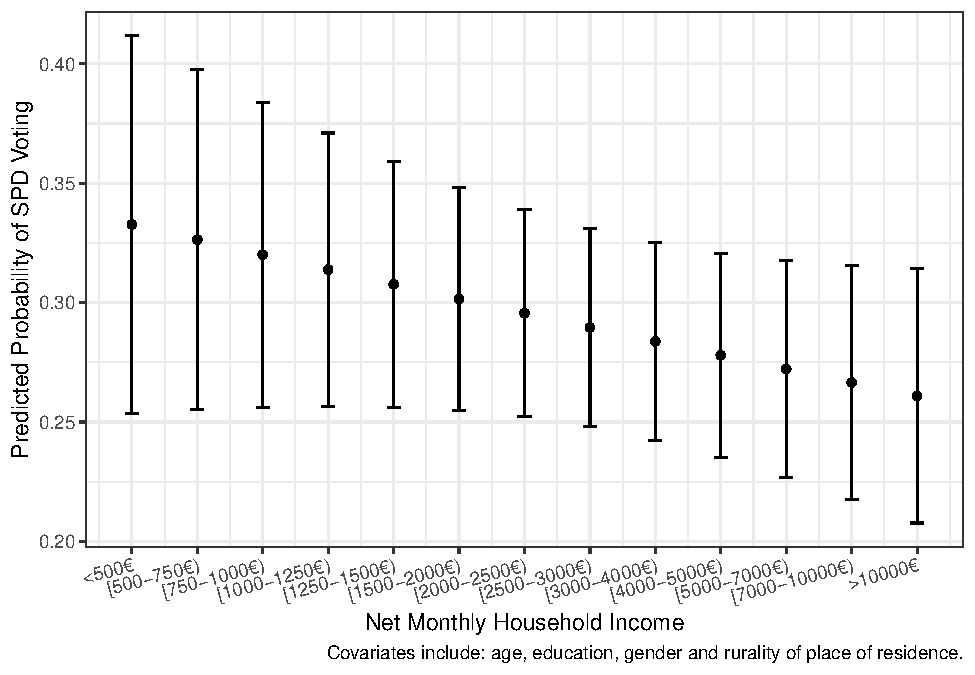
\includegraphics{AVCD_Final_Assignment-Edenhofer_files/figure-latex/spd-household-income-1.pdf}

There is no robust relationship between net monthly household income and
voting for the SPD.

Relationship between subjective class and SPD voting

\begin{Shaded}
\begin{Highlighting}[]
\NormalTok{spd\_sclass }\OtherTok{\textless{}{-}} \FunctionTok{glm}\NormalTok{(spd\_21 }\SpecialCharTok{\textasciitilde{}}\NormalTok{ subjective\_class }\SpecialCharTok{+}\NormalTok{ age }\SpecialCharTok{+}\NormalTok{ abitur\_factor }\SpecialCharTok{+}\NormalTok{ sex1 }\SpecialCharTok{+}\NormalTok{ urban\_rural\_factor }\SpecialCharTok{+}\NormalTok{ ostwest\_factor, }
                  \AttributeTok{family =} \FunctionTok{binomial}\NormalTok{(}\AttributeTok{link =} \StringTok{"logit"}\NormalTok{), }
                  \AttributeTok{data =}\NormalTok{ gles\_mod)}
\CommentTok{\# plot }
\FunctionTok{cplot}\NormalTok{(spd\_sclass, }\AttributeTok{x =} \StringTok{"subjective\_class"}\NormalTok{, }
      \AttributeTok{xvals =} \FunctionTok{seq}\NormalTok{(}\DecValTok{1}\NormalTok{, }\DecValTok{6}\NormalTok{, }\DecValTok{1}\NormalTok{), }\AttributeTok{draw =}\NormalTok{ F) }\SpecialCharTok{\%\textgreater{}\%}
  \FunctionTok{as\_tibble}\NormalTok{() }\SpecialCharTok{\%\textgreater{}\%}
  \FunctionTok{ggplot}\NormalTok{(}\FunctionTok{aes}\NormalTok{(}\AttributeTok{x =}\NormalTok{ xvals)) }\SpecialCharTok{+}
  \FunctionTok{geom\_point}\NormalTok{(}\FunctionTok{aes}\NormalTok{(}\AttributeTok{y =}\NormalTok{ yvals)) }\SpecialCharTok{+}
  \FunctionTok{geom\_errorbar}\NormalTok{(}\FunctionTok{aes}\NormalTok{(}\AttributeTok{ymin =}\NormalTok{ lower, }\AttributeTok{ymax =}\NormalTok{ upper), }\AttributeTok{width =} \FloatTok{0.2}\NormalTok{) }\SpecialCharTok{+}
  \FunctionTok{scale\_x\_continuous}\NormalTok{(}\StringTok{"Subjective Class"}\NormalTok{, }
                     \AttributeTok{breaks =} \FunctionTok{seq}\NormalTok{(}\DecValTok{1}\NormalTok{, }\DecValTok{6}\NormalTok{, }\DecValTok{1}\NormalTok{), }
                     \AttributeTok{labels =} \FunctionTok{c}\NormalTok{(}\StringTok{"Unterschicht"}\NormalTok{, }\StringTok{"Arbeiterschicht"}\NormalTok{, }
                                \StringTok{"Untere Mittelschicht"}\NormalTok{, }\StringTok{"mittlere Mittelschicht"}\NormalTok{, }
                                \StringTok{"obere Mittelschicht"}\NormalTok{, }\StringTok{"Oberschicht"}\NormalTok{)) }\SpecialCharTok{+}
  \FunctionTok{labs}\NormalTok{(}\AttributeTok{y =} \StringTok{"Predicted Probability of Voting SPD"}\NormalTok{, }
       \AttributeTok{caption =} \StringTok{"Covariates include: age, education, gender and rurality of place of residence."}\NormalTok{) }\SpecialCharTok{+}
  \FunctionTok{ylim}\NormalTok{(}\FunctionTok{c}\NormalTok{(}\FloatTok{0.1}\NormalTok{, }\FloatTok{0.5}\NormalTok{)) }\SpecialCharTok{+}
  \FunctionTok{theme\_bw}\NormalTok{() }\SpecialCharTok{+}
  \FunctionTok{theme}\NormalTok{(}\AttributeTok{axis.text.x =} \FunctionTok{element\_text}\NormalTok{(}\AttributeTok{angle =} \DecValTok{15}\NormalTok{, }\AttributeTok{hjust =} \DecValTok{1}\NormalTok{))}
\end{Highlighting}
\end{Shaded}

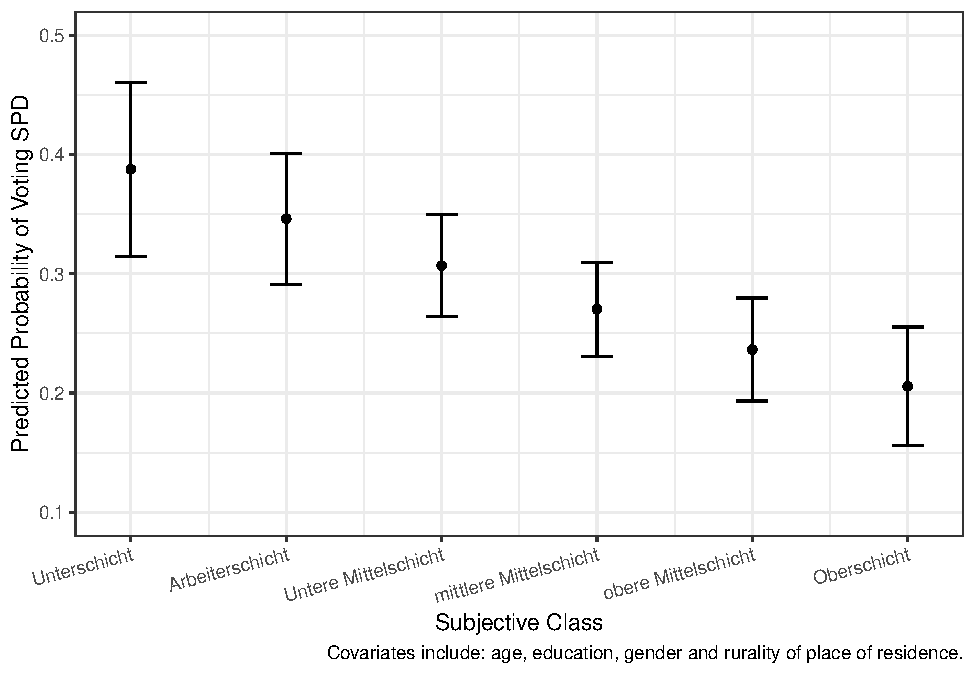
\includegraphics{AVCD_Final_Assignment-Edenhofer_files/figure-latex/spd-subjective-class-1.pdf}

What is the relationship between left-right self-placement and SPD
voting?

\begin{Shaded}
\begin{Highlighting}[]
\NormalTok{spd\_left\_right\_self }\OtherTok{\textless{}{-}} \FunctionTok{glm}\NormalTok{(spd\_21 }\SpecialCharTok{\textasciitilde{}}\NormalTok{ left\_right\_self }\SpecialCharTok{+} \FunctionTok{I}\NormalTok{(left\_right\_self}\SpecialCharTok{\^{}}\DecValTok{2}\NormalTok{) }\SpecialCharTok{+}\NormalTok{ household\_income }\SpecialCharTok{+}\NormalTok{ age }\SpecialCharTok{+}\NormalTok{ abitur\_factor }\SpecialCharTok{+}\NormalTok{ sex1 }\SpecialCharTok{+}\NormalTok{ urban\_rural\_factor }\SpecialCharTok{+}\NormalTok{ ostwest\_factor, }
                           \AttributeTok{family =} \FunctionTok{binomial}\NormalTok{(}\AttributeTok{link =} \StringTok{"logit"}\NormalTok{), }
                           \AttributeTok{data =}\NormalTok{ gles\_mod)}
\CommentTok{\# plot }
\FunctionTok{cplot}\NormalTok{(spd\_left\_right\_self, }\AttributeTok{x =} \StringTok{"left\_right\_self"}\NormalTok{, }
      \AttributeTok{xvals =} \FunctionTok{seq}\NormalTok{(}\DecValTok{1}\NormalTok{, }\DecValTok{11}\NormalTok{, }\DecValTok{1}\NormalTok{), }\AttributeTok{draw =}\NormalTok{ F) }\SpecialCharTok{\%\textgreater{}\%}
  \FunctionTok{as\_tibble}\NormalTok{() }\SpecialCharTok{\%\textgreater{}\%}
  \FunctionTok{ggplot}\NormalTok{(}\FunctionTok{aes}\NormalTok{(}\AttributeTok{x =}\NormalTok{ xvals)) }\SpecialCharTok{+}
  \FunctionTok{geom\_point}\NormalTok{(}\FunctionTok{aes}\NormalTok{(}\AttributeTok{y =}\NormalTok{ yvals)) }\SpecialCharTok{+}
  \FunctionTok{geom\_errorbar}\NormalTok{(}\FunctionTok{aes}\NormalTok{(}\AttributeTok{ymin =}\NormalTok{ lower, }\AttributeTok{ymax =}\NormalTok{ upper), }\AttributeTok{width =} \FloatTok{0.2}\NormalTok{) }\SpecialCharTok{+}
  \FunctionTok{scale\_x\_continuous}\NormalTok{(}\StringTok{"Left{-}Right Self{-}Placement"}\NormalTok{, }
                     \AttributeTok{breaks =} \FunctionTok{seq}\NormalTok{(}\DecValTok{1}\NormalTok{, }\DecValTok{11}\NormalTok{, }\DecValTok{1}\NormalTok{)) }\SpecialCharTok{+}
  \FunctionTok{expand\_limits}\NormalTok{(}\AttributeTok{y =} \FloatTok{0.5}\NormalTok{) }\SpecialCharTok{+}
  \FunctionTok{labs}\NormalTok{(}\AttributeTok{y =} \StringTok{"Predicted Probability of Voting SPD"}\NormalTok{) }\SpecialCharTok{+}
  \FunctionTok{theme\_bw}\NormalTok{()}
\end{Highlighting}
\end{Shaded}

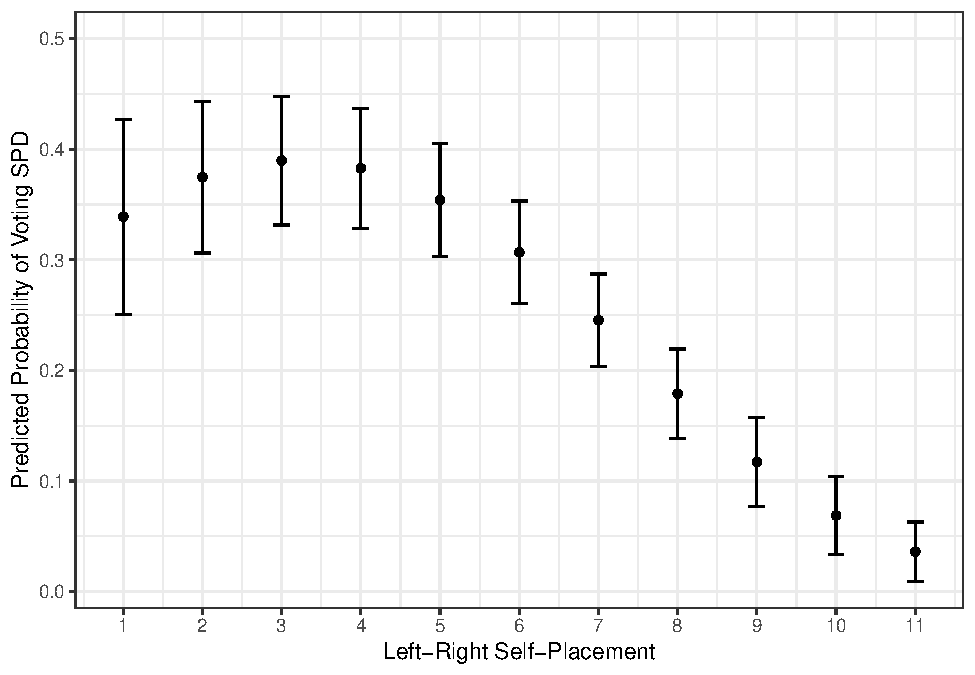
\includegraphics{AVCD_Final_Assignment-Edenhofer_files/figure-latex/spd-left-right-self-placement-1.pdf}

Relationship between age and SPD voting

\begin{Shaded}
\begin{Highlighting}[]
\NormalTok{spd\_age }\OtherTok{\textless{}{-}} \FunctionTok{glm}\NormalTok{(spd\_21 }\SpecialCharTok{\textasciitilde{}}\NormalTok{ household\_income }\SpecialCharTok{+}\NormalTok{ age }\SpecialCharTok{+}\NormalTok{ abitur\_factor }\SpecialCharTok{+}\NormalTok{ sex1 }\SpecialCharTok{+}\NormalTok{ urban\_rural\_factor }\SpecialCharTok{+}\NormalTok{ ostwest\_factor, }
               \AttributeTok{family =} \FunctionTok{binomial}\NormalTok{(}\AttributeTok{link =} \StringTok{"logit"}\NormalTok{), }
               \AttributeTok{data =}\NormalTok{ gles\_mod)}
\CommentTok{\# plot }
\FunctionTok{cplot}\NormalTok{(spd\_age, }\AttributeTok{x =} \StringTok{"age"}\NormalTok{, }\AttributeTok{draw =}\NormalTok{ F) }\SpecialCharTok{\%\textgreater{}\%}
  \FunctionTok{as\_tibble}\NormalTok{() }\SpecialCharTok{\%\textgreater{}\%}
  \FunctionTok{ggplot}\NormalTok{(}\FunctionTok{aes}\NormalTok{(}\AttributeTok{x =}\NormalTok{ xvals)) }\SpecialCharTok{+}
  \FunctionTok{geom\_line}\NormalTok{(}\FunctionTok{aes}\NormalTok{(}\AttributeTok{y =}\NormalTok{ yvals)) }\SpecialCharTok{+}
  \FunctionTok{geom\_ribbon}\NormalTok{(}\FunctionTok{aes}\NormalTok{(}\AttributeTok{ymin =}\NormalTok{ lower, }\AttributeTok{ymax =}\NormalTok{ upper), }\AttributeTok{alpha =} \FloatTok{0.2}\NormalTok{) }\SpecialCharTok{+}
  \FunctionTok{scale\_x\_continuous}\NormalTok{(}\StringTok{"Age"}\NormalTok{, }\AttributeTok{breaks =} \FunctionTok{seq}\NormalTok{(}\DecValTok{20}\NormalTok{, }\DecValTok{90}\NormalTok{, }\DecValTok{10}\NormalTok{)) }\SpecialCharTok{+}
  \FunctionTok{labs}\NormalTok{(}\AttributeTok{y =} \StringTok{"Predicted Probability of Voting SPD"}\NormalTok{) }\SpecialCharTok{+}
  \FunctionTok{theme\_bw}\NormalTok{()}
\end{Highlighting}
\end{Shaded}

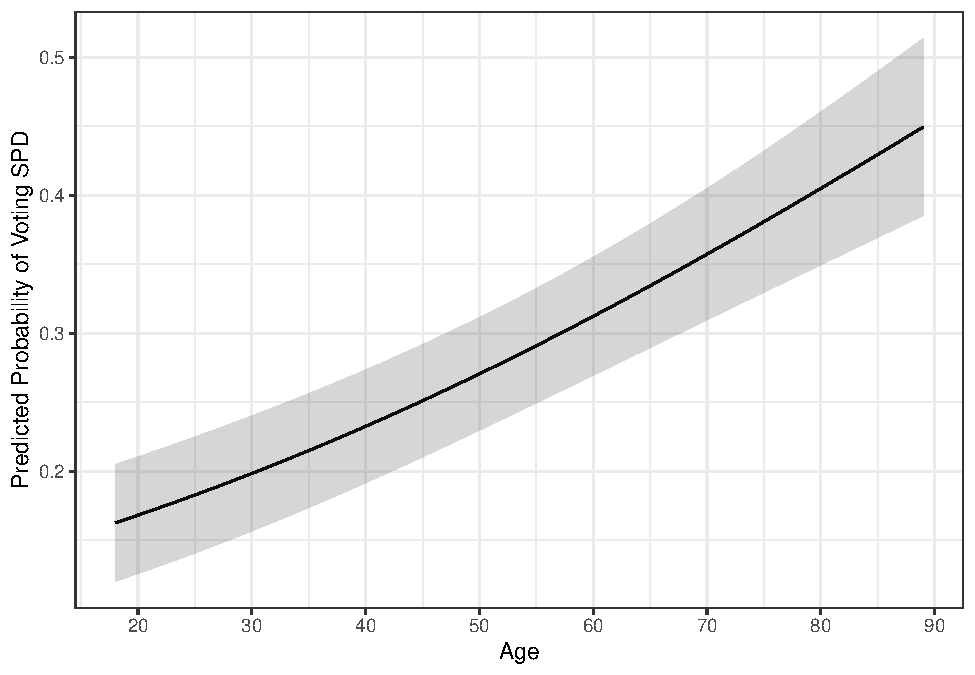
\includegraphics{AVCD_Final_Assignment-Edenhofer_files/figure-latex/spd-age-1.pdf}

Relationship between sex and SPD voting

\begin{Shaded}
\begin{Highlighting}[]
\FunctionTok{cplot}\NormalTok{(spd\_income, }\AttributeTok{x =} \StringTok{"sex1"}\NormalTok{, }\AttributeTok{draw =}\NormalTok{ F) }\SpecialCharTok{\%\textgreater{}\%}
  \FunctionTok{as\_tibble}\NormalTok{() }\SpecialCharTok{\%\textgreater{}\%}
  \FunctionTok{ggplot}\NormalTok{(}\FunctionTok{aes}\NormalTok{(}\AttributeTok{x =}\NormalTok{ xvals)) }\SpecialCharTok{+}
  \FunctionTok{geom\_point}\NormalTok{(}\FunctionTok{aes}\NormalTok{(}\AttributeTok{y =}\NormalTok{ yvals)) }\SpecialCharTok{+}
  \FunctionTok{geom\_errorbar}\NormalTok{(}\FunctionTok{aes}\NormalTok{(}\AttributeTok{ymin =}\NormalTok{ lower, }\AttributeTok{ymax =}\NormalTok{ upper), }\AttributeTok{width =} \FloatTok{0.2}\NormalTok{) }\SpecialCharTok{+}
  \FunctionTok{ylim}\NormalTok{(}\FunctionTok{c}\NormalTok{(}\FloatTok{0.2}\NormalTok{, }\FloatTok{0.4}\NormalTok{)) }\SpecialCharTok{+}
  \FunctionTok{scale\_x\_discrete}\NormalTok{(}\StringTok{"Sex"}\NormalTok{, }\AttributeTok{labels =} \FunctionTok{c}\NormalTok{(}\StringTok{"Female"}\NormalTok{, }\StringTok{"Male"}\NormalTok{)) }\SpecialCharTok{+}
  \FunctionTok{labs}\NormalTok{(}\AttributeTok{y =} \StringTok{"Predicted Probability of Voting SPD"}\NormalTok{) }\SpecialCharTok{+}
  \FunctionTok{theme\_bw}\NormalTok{()}
\end{Highlighting}
\end{Shaded}

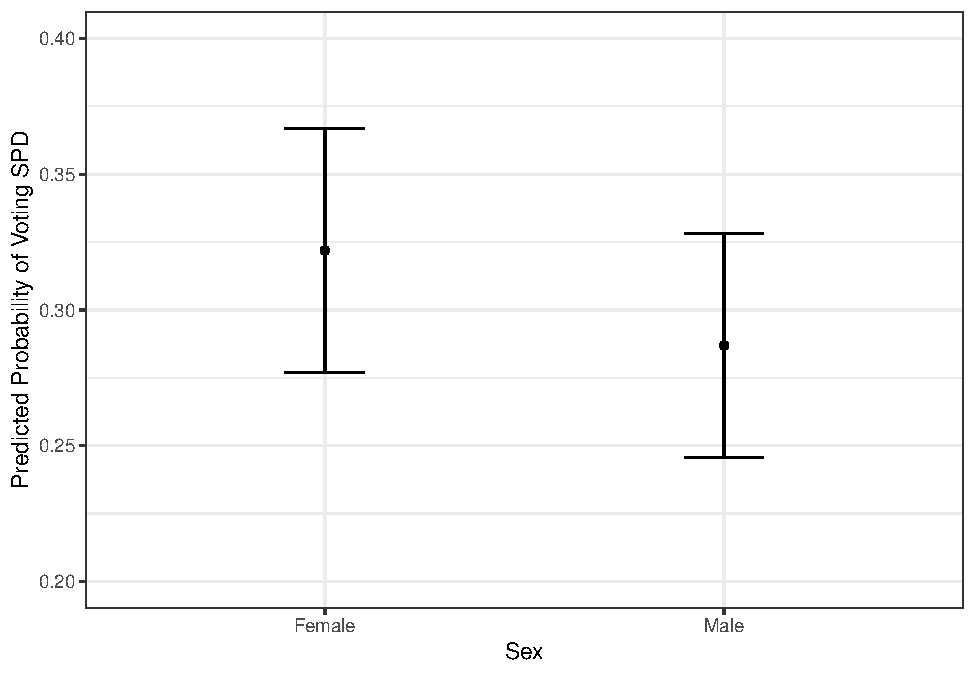
\includegraphics{AVCD_Final_Assignment-Edenhofer_files/figure-latex/spd-sex-1.pdf}

Relationship between education and SPD

\begin{Shaded}
\begin{Highlighting}[]
\FunctionTok{cplot}\NormalTok{(spd\_income, }\AttributeTok{x =} \StringTok{"abitur\_factor"}\NormalTok{, }\AttributeTok{draw =}\NormalTok{ F) }\SpecialCharTok{\%\textgreater{}\%}
  \FunctionTok{as\_tibble}\NormalTok{() }\SpecialCharTok{\%\textgreater{}\%}
  \FunctionTok{ggplot}\NormalTok{(}\FunctionTok{aes}\NormalTok{(}\AttributeTok{x =}\NormalTok{ xvals)) }\SpecialCharTok{+}
  \FunctionTok{geom\_point}\NormalTok{(}\FunctionTok{aes}\NormalTok{(}\AttributeTok{y =}\NormalTok{ yvals)) }\SpecialCharTok{+}
  \FunctionTok{geom\_errorbar}\NormalTok{(}\FunctionTok{aes}\NormalTok{(}\AttributeTok{ymin =}\NormalTok{ lower, }\AttributeTok{ymax =}\NormalTok{ upper), }\AttributeTok{width =} \FloatTok{0.2}\NormalTok{) }\SpecialCharTok{+} 
  \FunctionTok{scale\_x\_discrete}\NormalTok{(}\StringTok{"Education"}\NormalTok{, }\AttributeTok{labels =} \FunctionTok{c}\NormalTok{(}\StringTok{"At Least Abitur"}\NormalTok{, }\StringTok{"No Abitur"}\NormalTok{)) }\SpecialCharTok{+}
  \FunctionTok{ylim}\NormalTok{(}\FunctionTok{c}\NormalTok{(}\FloatTok{0.2}\NormalTok{, }\FloatTok{0.4}\NormalTok{)) }\SpecialCharTok{+}
  \FunctionTok{labs}\NormalTok{(}\AttributeTok{y =} \StringTok{"Predicted Probability of SPD Voting"}\NormalTok{) }\SpecialCharTok{+}
  \FunctionTok{theme\_bw}\NormalTok{()}
\end{Highlighting}
\end{Shaded}

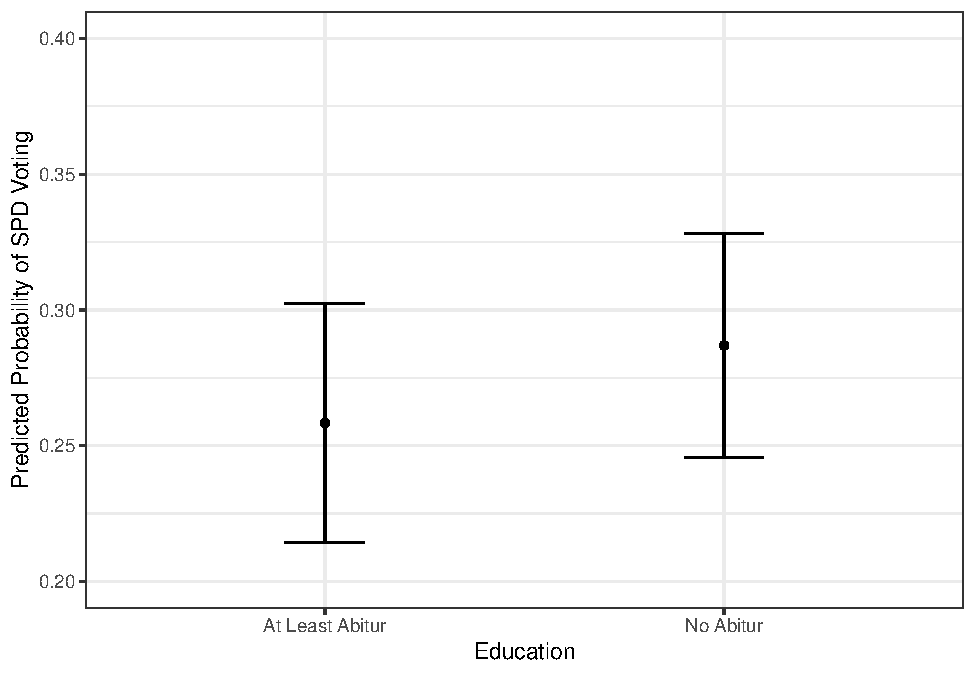
\includegraphics{AVCD_Final_Assignment-Edenhofer_files/figure-latex/spd-education-1.pdf}

\begin{Shaded}
\begin{Highlighting}[]
\FunctionTok{cplot}\NormalTok{(spd\_income, }\AttributeTok{x =} \StringTok{"ostwest\_factor"}\NormalTok{, }\AttributeTok{draw =}\NormalTok{ F) }\SpecialCharTok{\%\textgreater{}\%}
  \FunctionTok{as\_tibble}\NormalTok{() }\SpecialCharTok{\%\textgreater{}\%}
  \FunctionTok{ggplot}\NormalTok{(}\FunctionTok{aes}\NormalTok{(}\AttributeTok{x =}\NormalTok{ xvals)) }\SpecialCharTok{+}
  \FunctionTok{geom\_point}\NormalTok{(}\FunctionTok{aes}\NormalTok{(}\AttributeTok{y =}\NormalTok{ yvals)) }\SpecialCharTok{+}
  \FunctionTok{geom\_errorbar}\NormalTok{(}\FunctionTok{aes}\NormalTok{(}\AttributeTok{ymin =}\NormalTok{ lower, }\AttributeTok{ymax =}\NormalTok{ upper), }\AttributeTok{width =} \FloatTok{0.2}\NormalTok{) }\SpecialCharTok{+}
  \FunctionTok{scale\_x\_discrete}\NormalTok{(}\StringTok{"Ost{-}West Dummy"}\NormalTok{, }\AttributeTok{labels =} \FunctionTok{c}\NormalTok{(}\StringTok{"Ost"}\NormalTok{, }\StringTok{"West"}\NormalTok{)) }\SpecialCharTok{+}
  \FunctionTok{ylim}\NormalTok{(}\FunctionTok{c}\NormalTok{(}\FloatTok{0.2}\NormalTok{, }\FloatTok{0.4}\NormalTok{)) }\SpecialCharTok{+}
  \FunctionTok{labs}\NormalTok{(}\AttributeTok{y =} \StringTok{"Predicted Probability of Voting SPD"}\NormalTok{) }\SpecialCharTok{+}
  \FunctionTok{theme\_bw}\NormalTok{()}
\end{Highlighting}
\end{Shaded}

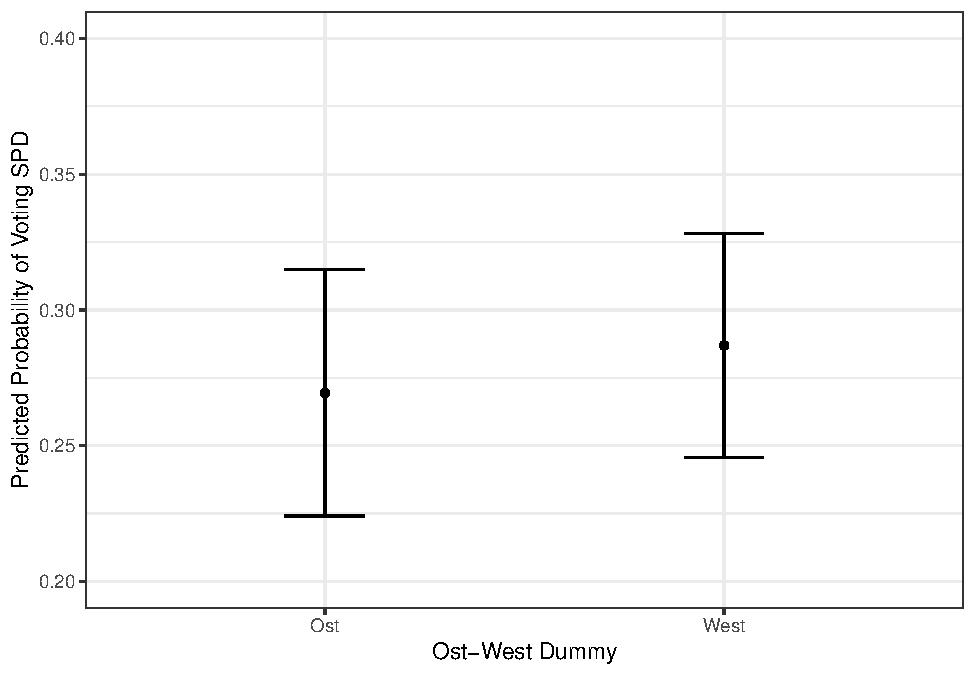
\includegraphics{AVCD_Final_Assignment-Edenhofer_files/figure-latex/spd-ost-west-1.pdf}

\hypertarget{attiudinal-correlates}{%
\subsubsection{Attiudinal Correlates}\label{attiudinal-correlates}}

\begin{Shaded}
\begin{Highlighting}[]
\CommentTok{\# none of the other abgehaengt variables is significant }
\NormalTok{spd\_cancel\_culture }\OtherTok{\textless{}{-}} \FunctionTok{glm}\NormalTok{(spd\_21 }\SpecialCharTok{\textasciitilde{}}\NormalTok{ cancel\_culture\_subjektiv }\SpecialCharTok{+}\NormalTok{ household\_income }\SpecialCharTok{+}\NormalTok{ age }\SpecialCharTok{+}\NormalTok{ abitur\_factor }\SpecialCharTok{+}\NormalTok{ sex1 }\SpecialCharTok{+}\NormalTok{ urban\_rural\_factor }\SpecialCharTok{+}\NormalTok{ ostwest\_factor, }\AttributeTok{family =} \FunctionTok{binomial}\NormalTok{(}\AttributeTok{link =} \StringTok{"logit"}\NormalTok{), }\AttributeTok{data =}\NormalTok{ gles\_mod)}
\CommentTok{\# plot }
\FunctionTok{cplot}\NormalTok{(spd\_cancel\_culture, }\AttributeTok{x =} \StringTok{"cancel\_culture\_subjektiv"}\NormalTok{, }
      \AttributeTok{xvals =} \FunctionTok{seq}\NormalTok{(}\DecValTok{1}\NormalTok{, }\DecValTok{5}\NormalTok{, }\DecValTok{1}\NormalTok{), }\AttributeTok{draw =}\NormalTok{ F) }\SpecialCharTok{\%\textgreater{}\%} 
  \FunctionTok{as\_tibble}\NormalTok{() }\SpecialCharTok{\%\textgreater{}\%}
  \FunctionTok{ggplot}\NormalTok{(}\FunctionTok{aes}\NormalTok{(}\AttributeTok{x =}\NormalTok{ xvals)) }\SpecialCharTok{+}
  \FunctionTok{geom\_point}\NormalTok{(}\FunctionTok{aes}\NormalTok{(}\AttributeTok{y =}\NormalTok{ yvals)) }\SpecialCharTok{+}
  \FunctionTok{geom\_errorbar}\NormalTok{(}\FunctionTok{aes}\NormalTok{(}\AttributeTok{ymin =}\NormalTok{ lower, }\AttributeTok{ymax =}\NormalTok{ upper), }\AttributeTok{width =} \FloatTok{0.2}\NormalTok{) }\SpecialCharTok{+}
  \FunctionTok{scale\_x\_continuous}\NormalTok{(}\StringTok{"Subjektiv: Keine freie Meinungsaeusserung moeglich"}\NormalTok{, }
                   \AttributeTok{breaks =} \FunctionTok{seq}\NormalTok{(}\DecValTok{1}\NormalTok{, }\DecValTok{5}\NormalTok{, }\DecValTok{1}\NormalTok{),}
                   \AttributeTok{labels =} \FunctionTok{c}\NormalTok{(}\StringTok{"Stimme voll zu"}\NormalTok{, }\StringTok{"Stimme eher zu"}\NormalTok{,}
                              \StringTok{"teils/teils"}\NormalTok{, }\StringTok{"Stimme eher nicht zu"}\NormalTok{,}
                              \StringTok{"Stimme ueberhaupt nicht zu"}\NormalTok{)) }\SpecialCharTok{+}
  \FunctionTok{labs}\NormalTok{(}\AttributeTok{y =} \StringTok{"Predicted Probability of Voting SPD"}\NormalTok{) }\SpecialCharTok{+}
  \FunctionTok{ylim}\NormalTok{(}\FunctionTok{c}\NormalTok{(}\FloatTok{0.1}\NormalTok{, }\FloatTok{0.4}\NormalTok{)) }\SpecialCharTok{+}
  \FunctionTok{theme\_bw}\NormalTok{() }\SpecialCharTok{+}
  \FunctionTok{theme}\NormalTok{(}\AttributeTok{axis.text.x =} \FunctionTok{element\_text}\NormalTok{(}\AttributeTok{angle =} \DecValTok{15}\NormalTok{, }\AttributeTok{hjust =} \DecValTok{1}\NormalTok{))}
\end{Highlighting}
\end{Shaded}

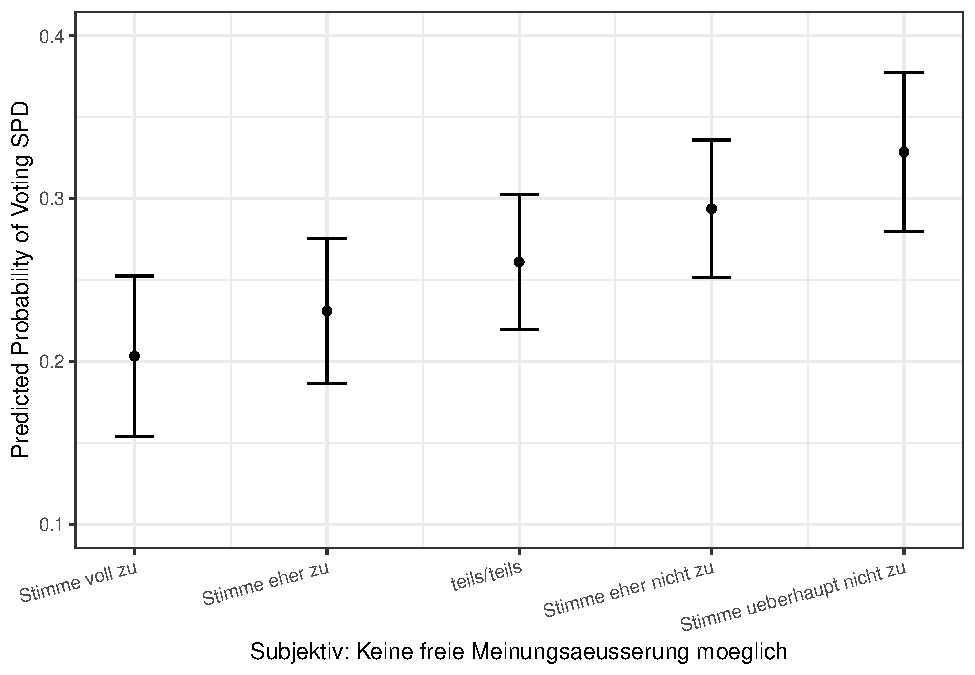
\includegraphics{AVCD_Final_Assignment-Edenhofer_files/figure-latex/spd-cancel-culture-1.pdf}

\begin{Shaded}
\begin{Highlighting}[]
\CommentTok{\# general trust is not significant }
\CommentTok{\# trust in parliament is significant }
\NormalTok{spd\_trust\_parliament }\OtherTok{\textless{}{-}} \FunctionTok{glm}\NormalTok{(spd\_21 }\SpecialCharTok{\textasciitilde{}}\NormalTok{ trust\_in\_parliament }\SpecialCharTok{+} \FunctionTok{I}\NormalTok{(trust\_in\_parliament}\SpecialCharTok{\^{}}\DecValTok{2}\NormalTok{) }\SpecialCharTok{+}\NormalTok{ household\_income }\SpecialCharTok{+}\NormalTok{ age }\SpecialCharTok{+}\NormalTok{ abitur\_factor }\SpecialCharTok{+}\NormalTok{ sex1 }\SpecialCharTok{+}\NormalTok{ urban\_rural\_factor }\SpecialCharTok{+}\NormalTok{ ostwest\_factor, }\AttributeTok{family =} \FunctionTok{binomial}\NormalTok{(}\AttributeTok{link =} \StringTok{"logit"}\NormalTok{), }\AttributeTok{data =}\NormalTok{ gles\_mod)}
\CommentTok{\# plot }
\FunctionTok{cplot}\NormalTok{(spd\_trust\_parliament, }\AttributeTok{x =} \StringTok{"trust\_in\_parliament"}\NormalTok{, }
      \AttributeTok{xvals =} \FunctionTok{seq}\NormalTok{(}\DecValTok{1}\NormalTok{, }\DecValTok{11}\NormalTok{, }\DecValTok{1}\NormalTok{), }\AttributeTok{draw =}\NormalTok{ F) }\SpecialCharTok{\%\textgreater{}\%}
  \FunctionTok{as\_tibble}\NormalTok{() }\SpecialCharTok{\%\textgreater{}\%}
  \FunctionTok{ggplot}\NormalTok{(}\FunctionTok{aes}\NormalTok{(}\AttributeTok{x =}\NormalTok{ xvals)) }\SpecialCharTok{+}
  \FunctionTok{geom\_point}\NormalTok{(}\FunctionTok{aes}\NormalTok{(}\AttributeTok{y =}\NormalTok{ yvals)) }\SpecialCharTok{+}
  \FunctionTok{geom\_errorbar}\NormalTok{(}\FunctionTok{aes}\NormalTok{(}\AttributeTok{ymin =}\NormalTok{ lower, }\AttributeTok{ymax =}\NormalTok{ upper), }\AttributeTok{width =} \FloatTok{0.2}\NormalTok{) }\SpecialCharTok{+}
  \FunctionTok{scale\_x\_continuous}\NormalTok{(}\StringTok{"Vertrauen: Bundestag"}\NormalTok{, }
                     \AttributeTok{breaks =} \FunctionTok{seq}\NormalTok{(}\DecValTok{1}\NormalTok{, }\DecValTok{11}\NormalTok{, }\DecValTok{1}\NormalTok{)) }\SpecialCharTok{+}
  \FunctionTok{labs}\NormalTok{(}\AttributeTok{y =} \StringTok{"Predicted Probability of Voting SPD"}\NormalTok{, }
       \AttributeTok{caption =} \StringTok{"\textquotesingle{}1\textquotesingle{} indicates \textquotesingle{}no trust\textquotesingle{}, while 11 indicates \textquotesingle{}full trust\textquotesingle{}."}\NormalTok{) }\SpecialCharTok{+}
  \FunctionTok{ylim}\NormalTok{(}\FunctionTok{c}\NormalTok{(}\DecValTok{0}\NormalTok{, }\FloatTok{0.4}\NormalTok{)) }\SpecialCharTok{+}
  \FunctionTok{theme\_bw}\NormalTok{()}
\end{Highlighting}
\end{Shaded}

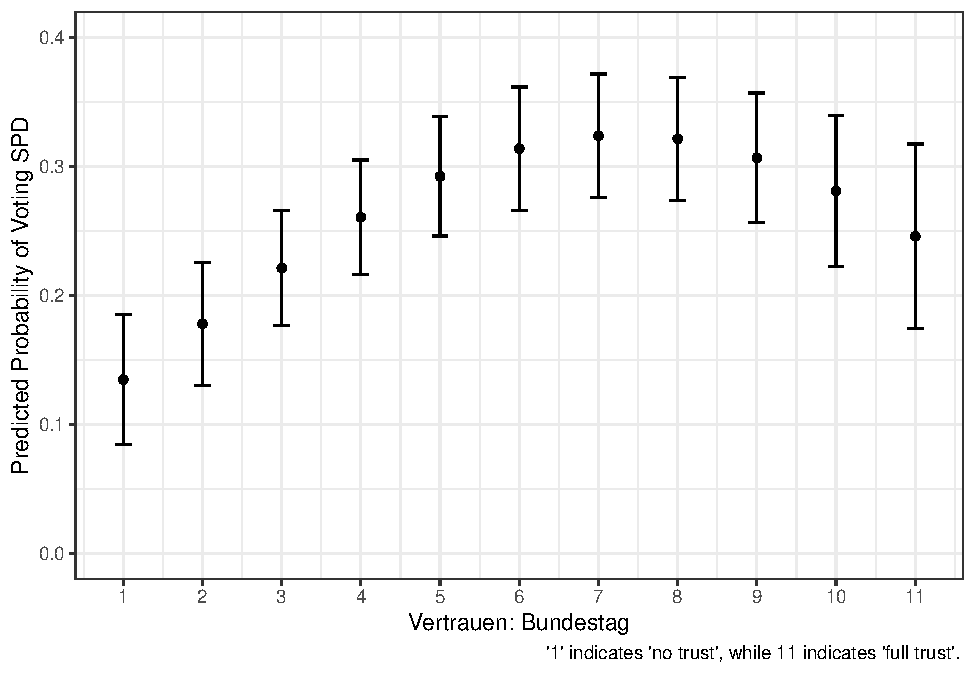
\includegraphics{AVCD_Final_Assignment-Edenhofer_files/figure-latex/spd-trust-parliament-1.pdf}

\begin{Shaded}
\begin{Highlighting}[]
\CommentTok{\# trust in parties }
\NormalTok{spd\_trust\_parties }\OtherTok{\textless{}{-}} \FunctionTok{glm}\NormalTok{(spd\_21 }\SpecialCharTok{\textasciitilde{}}\NormalTok{ trust\_in\_parties }\SpecialCharTok{+} \FunctionTok{I}\NormalTok{(trust\_in\_parties}\SpecialCharTok{\^{}}\DecValTok{2}\NormalTok{) }\SpecialCharTok{+}\NormalTok{ household\_income }\SpecialCharTok{+}\NormalTok{ age }\SpecialCharTok{+}\NormalTok{ abitur\_factor }\SpecialCharTok{+}\NormalTok{ sex1 }\SpecialCharTok{+}\NormalTok{ urban\_rural\_factor }\SpecialCharTok{+}\NormalTok{ ostwest\_factor, }\AttributeTok{family =} \FunctionTok{binomial}\NormalTok{(}\AttributeTok{link =} \StringTok{"logit"}\NormalTok{), }\AttributeTok{data =}\NormalTok{ gles\_mod)}
\CommentTok{\# plot }
\FunctionTok{cplot}\NormalTok{(spd\_trust\_parties, }\AttributeTok{x =} \StringTok{"trust\_in\_parties"}\NormalTok{, }
      \AttributeTok{xvals =} \FunctionTok{seq}\NormalTok{(}\DecValTok{1}\NormalTok{, }\DecValTok{11}\NormalTok{, }\DecValTok{1}\NormalTok{), }\AttributeTok{draw =}\NormalTok{ F) }\SpecialCharTok{\%\textgreater{}\%}
  \FunctionTok{as\_tibble}\NormalTok{() }\SpecialCharTok{\%\textgreater{}\%}
  \FunctionTok{ggplot}\NormalTok{(}\FunctionTok{aes}\NormalTok{(}\AttributeTok{x =}\NormalTok{ xvals)) }\SpecialCharTok{+}
  \FunctionTok{geom\_point}\NormalTok{(}\FunctionTok{aes}\NormalTok{(}\AttributeTok{y =}\NormalTok{ yvals)) }\SpecialCharTok{+}
  \FunctionTok{geom\_errorbar}\NormalTok{(}\FunctionTok{aes}\NormalTok{(}\AttributeTok{ymin =}\NormalTok{ lower, }\AttributeTok{ymax =}\NormalTok{ upper), }\AttributeTok{width =} \FloatTok{0.2}\NormalTok{) }\SpecialCharTok{+}
  \FunctionTok{scale\_x\_continuous}\NormalTok{(}\StringTok{"Vertrauen: Parteien"}\NormalTok{, }
                     \AttributeTok{breaks =} \FunctionTok{seq}\NormalTok{(}\DecValTok{1}\NormalTok{, }\DecValTok{11}\NormalTok{, }\DecValTok{1}\NormalTok{)) }\SpecialCharTok{+}
  \FunctionTok{labs}\NormalTok{(}\AttributeTok{y =} \StringTok{"Predicted Probability of Voting SPD"}\NormalTok{, }
       \AttributeTok{caption =} \StringTok{"\textquotesingle{}1\textquotesingle{} indicates \textquotesingle{}no trust\textquotesingle{}, while 11 indicates \textquotesingle{}full trust\textquotesingle{}."}\NormalTok{) }\SpecialCharTok{+}
  \FunctionTok{ylim}\NormalTok{(}\FunctionTok{c}\NormalTok{(}\DecValTok{0}\NormalTok{, }\FloatTok{0.4}\NormalTok{)) }\SpecialCharTok{+}
  \FunctionTok{theme\_bw}\NormalTok{()}
\end{Highlighting}
\end{Shaded}

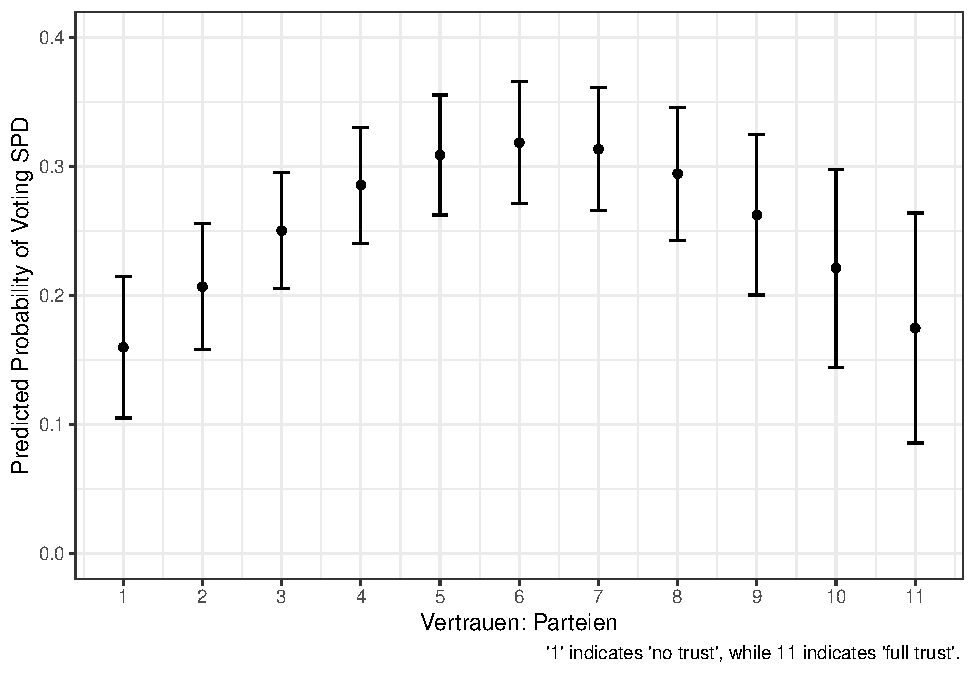
\includegraphics{AVCD_Final_Assignment-Edenhofer_files/figure-latex/spd-trust-parties-1.pdf}

\begin{Shaded}
\begin{Highlighting}[]
\CommentTok{\# trust in politicians}
\NormalTok{spd\_trust\_politicians }\OtherTok{\textless{}{-}} \FunctionTok{glm}\NormalTok{(spd\_21 }\SpecialCharTok{\textasciitilde{}}\NormalTok{ trust\_in\_politicians }\SpecialCharTok{+} \FunctionTok{I}\NormalTok{(trust\_in\_politicians}\SpecialCharTok{\^{}}\DecValTok{2}\NormalTok{) }\SpecialCharTok{+}\NormalTok{ household\_income }\SpecialCharTok{+}\NormalTok{ age }\SpecialCharTok{+}\NormalTok{ abitur\_factor }\SpecialCharTok{+}\NormalTok{ sex1 }\SpecialCharTok{+}\NormalTok{ urban\_rural\_factor }\SpecialCharTok{+}\NormalTok{ ostwest\_factor, }\AttributeTok{family =} \FunctionTok{binomial}\NormalTok{(}\AttributeTok{link =} \StringTok{"logit"}\NormalTok{), }\AttributeTok{data =}\NormalTok{ gles\_mod)}
\CommentTok{\# plot }
\FunctionTok{cplot}\NormalTok{(spd\_trust\_politicians, }\AttributeTok{x =} \StringTok{"trust\_in\_politicians"}\NormalTok{,}
      \AttributeTok{xvals =} \FunctionTok{seq}\NormalTok{(}\DecValTok{1}\NormalTok{, }\DecValTok{11}\NormalTok{, }\DecValTok{1}\NormalTok{), }\AttributeTok{draw =}\NormalTok{ F) }\SpecialCharTok{\%\textgreater{}\%}
  \FunctionTok{as\_tibble}\NormalTok{() }\SpecialCharTok{\%\textgreater{}\%}
  \FunctionTok{ggplot}\NormalTok{(}\FunctionTok{aes}\NormalTok{(}\AttributeTok{x =}\NormalTok{ xvals)) }\SpecialCharTok{+}
  \FunctionTok{geom\_point}\NormalTok{(}\FunctionTok{aes}\NormalTok{(}\AttributeTok{y =}\NormalTok{ yvals)) }\SpecialCharTok{+}
  \FunctionTok{geom\_errorbar}\NormalTok{(}\FunctionTok{aes}\NormalTok{(}\AttributeTok{ymin =}\NormalTok{ lower, }\AttributeTok{ymax =}\NormalTok{ upper), }\AttributeTok{width =} \FloatTok{0.2}\NormalTok{) }\SpecialCharTok{+}
  \FunctionTok{scale\_x\_continuous}\NormalTok{(}\StringTok{"Vertrauen: Politiker:innen"}\NormalTok{, }
                     \AttributeTok{breaks =} \FunctionTok{seq}\NormalTok{(}\DecValTok{1}\NormalTok{, }\DecValTok{11}\NormalTok{, }\DecValTok{1}\NormalTok{)) }\SpecialCharTok{+}
  \FunctionTok{labs}\NormalTok{(}\AttributeTok{y =} \StringTok{"Predicted Probability of Voting SPD"}\NormalTok{, }
       \AttributeTok{caption =} \StringTok{"\textquotesingle{}1\textquotesingle{} indicates \textquotesingle{}no trust\textquotesingle{}, while 11 indicates \textquotesingle{}full trust\textquotesingle{}."}\NormalTok{) }\SpecialCharTok{+}
  \FunctionTok{ylim}\NormalTok{(}\FunctionTok{c}\NormalTok{(}\DecValTok{0}\NormalTok{, }\FloatTok{0.4}\NormalTok{)) }\SpecialCharTok{+}
  \FunctionTok{theme\_bw}\NormalTok{()}
\end{Highlighting}
\end{Shaded}

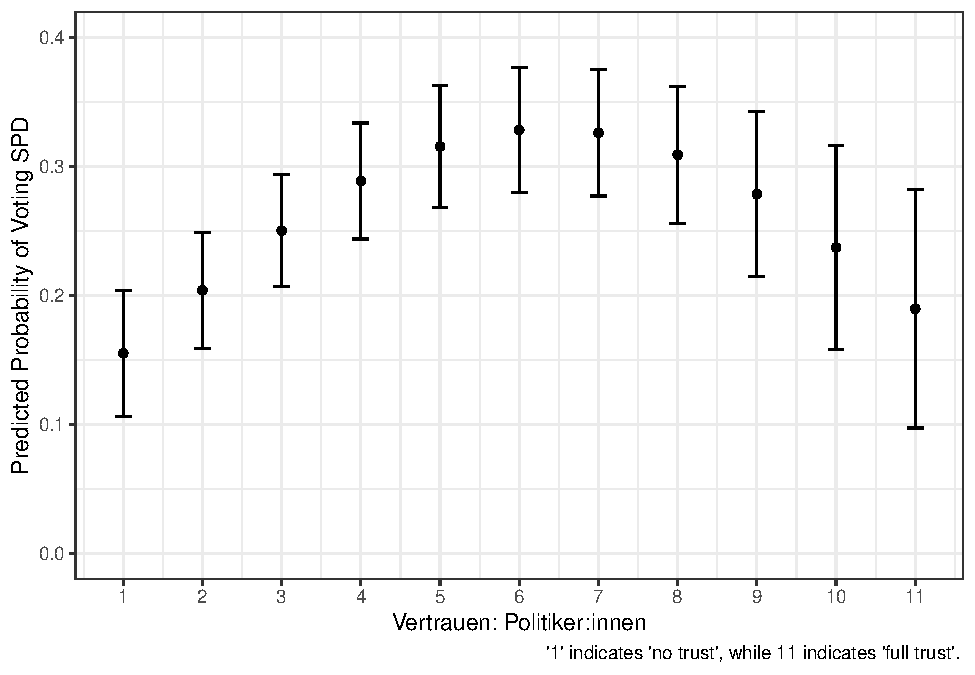
\includegraphics{AVCD_Final_Assignment-Edenhofer_files/figure-latex/spd-trust-politicians-1.pdf}

\begin{Shaded}
\begin{Highlighting}[]
\CommentTok{\# immigrants bring crime is significant }
\NormalTok{spd\_immig\_crime }\OtherTok{\textless{}{-}} \FunctionTok{glm}\NormalTok{(spd\_21 }\SpecialCharTok{\textasciitilde{}}\NormalTok{ out\_group\_immig\_crime }\SpecialCharTok{+}\NormalTok{ household\_income }\SpecialCharTok{+}\NormalTok{ age }\SpecialCharTok{+}\NormalTok{ abitur\_factor }\SpecialCharTok{+}\NormalTok{ sex1 }\SpecialCharTok{+}\NormalTok{ urban\_rural\_factor }\SpecialCharTok{+}\NormalTok{ ostwest\_factor, }\AttributeTok{family =} \FunctionTok{binomial}\NormalTok{(}\AttributeTok{link =} \StringTok{"logit"}\NormalTok{), }\AttributeTok{data =}\NormalTok{ gles\_mod)}
\CommentTok{\# plot }
\FunctionTok{cplot}\NormalTok{(spd\_immig\_crime, }\AttributeTok{x =} \StringTok{"out\_group\_immig\_crime"}\NormalTok{, }
      \AttributeTok{xvals =} \FunctionTok{seq}\NormalTok{(}\DecValTok{1}\NormalTok{, }\DecValTok{5}\NormalTok{, }\DecValTok{1}\NormalTok{), }\AttributeTok{draw =}\NormalTok{ F) }\SpecialCharTok{\%\textgreater{}\%}
  \FunctionTok{as\_tibble}\NormalTok{() }\SpecialCharTok{\%\textgreater{}\%}
  \FunctionTok{ggplot}\NormalTok{(}\FunctionTok{aes}\NormalTok{(}\AttributeTok{x =}\NormalTok{ xvals)) }\SpecialCharTok{+}
  \FunctionTok{geom\_point}\NormalTok{(}\FunctionTok{aes}\NormalTok{(}\AttributeTok{y =}\NormalTok{ yvals)) }\SpecialCharTok{+}
  \FunctionTok{geom\_errorbar}\NormalTok{(}\FunctionTok{aes}\NormalTok{(}\AttributeTok{ymin =}\NormalTok{ lower, }\AttributeTok{ymax =}\NormalTok{ upper), }\AttributeTok{width =} \FloatTok{0.2}\NormalTok{) }\SpecialCharTok{+}
  \FunctionTok{scale\_x\_continuous}\NormalTok{(}\StringTok{"Immigration erhoeht Kriminalitaet in BRD"}\NormalTok{, }
                     \AttributeTok{breaks =} \FunctionTok{seq}\NormalTok{(}\DecValTok{1}\NormalTok{, }\DecValTok{5}\NormalTok{, }\DecValTok{1}\NormalTok{), }
                     \AttributeTok{labels =} \FunctionTok{c}\NormalTok{(}\StringTok{"Stimme voll und ganz zu"}\NormalTok{, }\StringTok{"Stimme eher zu"}\NormalTok{, }
                                \StringTok{"Teils/Teils"}\NormalTok{, }\StringTok{"Lehne eher ab"}\NormalTok{, }
                                \StringTok{"Lehne voll und ganz ab"}\NormalTok{)) }\SpecialCharTok{+}
  \FunctionTok{labs}\NormalTok{(}\AttributeTok{y =} \StringTok{"Predicted Probability of Voting SPD"}\NormalTok{) }\SpecialCharTok{+}
  \FunctionTok{ylim}\NormalTok{(}\FunctionTok{c}\NormalTok{(}\FloatTok{0.1}\NormalTok{, }\FloatTok{0.4}\NormalTok{)) }\SpecialCharTok{+}
  \FunctionTok{theme\_bw}\NormalTok{() }
\end{Highlighting}
\end{Shaded}

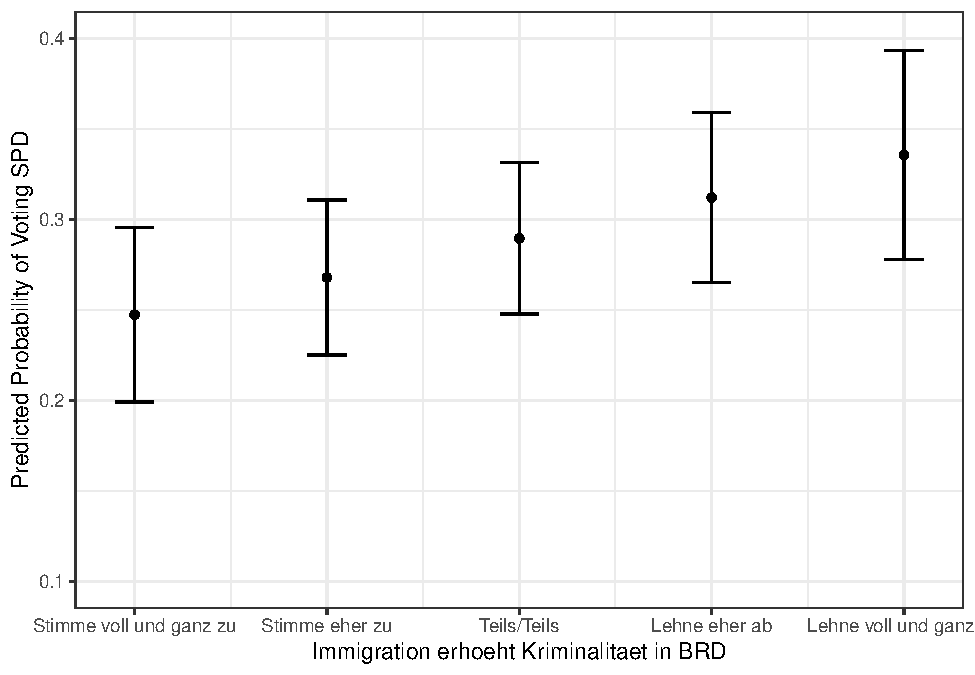
\includegraphics{AVCD_Final_Assignment-Edenhofer_files/figure-latex/spd-immig-crime-1.pdf}

\begin{Shaded}
\begin{Highlighting}[]
\CommentTok{\# immigrants pose cultural threat is not significant at 5\% level }
\CommentTok{\# immigrants are good for economics is not significant at 5\% level }
\CommentTok{\# majority will is paramount is not significant }
\CommentTok{\# outgroups should assimilate not significant }
\end{Highlighting}
\end{Shaded}

\hypertarget{gruene}{%
\subsection{Gruene}\label{gruene}}

\hypertarget{spatial-distance}{%
\subsubsection{Spatial distance}\label{spatial-distance}}

\begin{Shaded}
\begin{Highlighting}[]
\NormalTok{gruene\_space }\OtherTok{\textless{}{-}} \FunctionTok{glm}\NormalTok{(gruene\_21 }\SpecialCharTok{\textasciitilde{}}\NormalTok{ distance\_green }\SpecialCharTok{+}\NormalTok{ household\_income }\SpecialCharTok{+}\NormalTok{ age }\SpecialCharTok{+}\NormalTok{ abitur\_factor }\SpecialCharTok{+}\NormalTok{ sex1 }\SpecialCharTok{+}\NormalTok{ urban\_rural\_factor }\SpecialCharTok{+}\NormalTok{ ostwest\_factor, }\AttributeTok{family =} \FunctionTok{binomial}\NormalTok{(}\AttributeTok{link =} \StringTok{"logit"}\NormalTok{), }\AttributeTok{data =}\NormalTok{ gles\_mod)}


\FunctionTok{summary}\NormalTok{(gruene\_space)}
\end{Highlighting}
\end{Shaded}

\begin{verbatim}
## 
## Call:
## glm(formula = gruene_21 ~ distance_green + household_income + 
##     age + abitur_factor + sex1 + urban_rural_factor + ostwest_factor, 
##     family = binomial(link = "logit"), data = gles_mod)
## 
## Deviance Residuals: 
##     Min       1Q   Median       3Q      Max  
## -1.5342  -0.7083  -0.3949  -0.0132   4.0312  
## 
## Coefficients:
##                         Estimate Std. Error z value Pr(>|z|)    
## (Intercept)             0.163515   0.333388   0.490   0.6238    
## distance_green         -0.218754   0.021620 -10.118  < 2e-16 ***
## household_income        0.045328   0.026401   1.717   0.0860 .  
## age                    -0.021889   0.003562  -6.145 7.98e-10 ***
## abitur_factorno_abitur -0.750826   0.123852  -6.062 1.34e-09 ***
## sex1female              0.296052   0.115518   2.563   0.0104 *  
## urban_rural_factor2    -0.195854   0.182306  -1.074   0.2827    
## urban_rural_factor3    -0.326921   0.151903  -2.152   0.0314 *  
## urban_rural_factor4    -0.395278   0.162413  -2.434   0.0149 *  
## urban_rural_factor5     0.158309   0.576306   0.275   0.7835    
## ostwest_factorwest      0.596282   0.138086   4.318 1.57e-05 ***
## ---
## Signif. codes:  0 '***' 0.001 '**' 0.01 '*' 0.05 '.' 0.1 ' ' 1
## 
## (Dispersion parameter for binomial family taken to be 1)
## 
##     Null deviance: 2334.8  on 2243  degrees of freedom
## Residual deviance: 1848.4  on 2233  degrees of freedom
##   (1180 observations deleted due to missingness)
## AIC: 1870.4
## 
## Number of Fisher Scoring iterations: 7
\end{verbatim}

\begin{Shaded}
\begin{Highlighting}[]
\CommentTok{\# placement of greens }
\NormalTok{gles\_mod }\SpecialCharTok{\%\textgreater{}\%}
  \FunctionTok{select}\NormalTok{(left\_right\_green\_factor, left\_right\_self\_factor) }\SpecialCharTok{\%\textgreater{}\%}
  \FunctionTok{filter}\NormalTok{(}\SpecialCharTok{!}\FunctionTok{is.na}\NormalTok{(left\_right\_green\_factor) }\SpecialCharTok{\&} \SpecialCharTok{!}\FunctionTok{is.na}\NormalTok{(left\_right\_self\_factor)) }\SpecialCharTok{\%\textgreater{}\%}
  \FunctionTok{pivot\_longer}\NormalTok{(}\AttributeTok{cols =} \FunctionTok{everything}\NormalTok{(), }\AttributeTok{names\_to =} \StringTok{"type"}\NormalTok{, }\AttributeTok{values\_to =} \StringTok{"value"}\NormalTok{) }\SpecialCharTok{\%\textgreater{}\%}
  \FunctionTok{count}\NormalTok{(type, value) }\SpecialCharTok{\%\textgreater{}\%}
  \FunctionTok{group\_by}\NormalTok{(type) }\SpecialCharTok{\%\textgreater{}\%}
  \FunctionTok{mutate}\NormalTok{(}\AttributeTok{share =} \DecValTok{100}\SpecialCharTok{*}\NormalTok{(n}\SpecialCharTok{/}\FunctionTok{sum}\NormalTok{(n))) }\SpecialCharTok{\%\textgreater{}\%}
  \FunctionTok{ggplot}\NormalTok{(}\FunctionTok{aes}\NormalTok{(}\AttributeTok{x =}\NormalTok{ value, }\AttributeTok{y =}\NormalTok{ share, }\AttributeTok{fill =}\NormalTok{ type)) }\SpecialCharTok{+}
  \FunctionTok{geom\_col}\NormalTok{(}\AttributeTok{position =} \StringTok{"dodge"}\NormalTok{) }\SpecialCharTok{+}
  \FunctionTok{geom\_text}\NormalTok{(}\FunctionTok{aes}\NormalTok{(}\AttributeTok{label =} \FunctionTok{round}\NormalTok{(share, }\DecValTok{1}\NormalTok{)), }\AttributeTok{vjust =} \SpecialCharTok{{-}}\FloatTok{0.2}\NormalTok{, }\AttributeTok{size =} \FloatTok{2.7}\NormalTok{,}
            \AttributeTok{position =} \FunctionTok{position\_dodge}\NormalTok{(}\AttributeTok{width =} \FloatTok{0.8}\NormalTok{)) }\SpecialCharTok{+}
  \FunctionTok{scale\_y\_continuous}\NormalTok{(}\StringTok{"Share of respondents"}\NormalTok{, }\AttributeTok{labels =}\NormalTok{ scales}\SpecialCharTok{::}\FunctionTok{label\_percent}\NormalTok{(}\AttributeTok{scale =} \DecValTok{1}\NormalTok{)) }\SpecialCharTok{+}
  \FunctionTok{scale\_fill\_brewer}\NormalTok{(}\StringTok{""}\NormalTok{, }
                    \AttributeTok{labels =} \FunctionTok{c}\NormalTok{(}\StringTok{"left\_right\_green\_factor"} \OtherTok{=} \StringTok{"L{-}R placement of Greens"}\NormalTok{, }
                               \StringTok{"left\_right\_self\_factor"} \OtherTok{=} \StringTok{"Self L{-}R placement"}\NormalTok{)) }\SpecialCharTok{+}
  \FunctionTok{expand\_limits}\NormalTok{(}\AttributeTok{y =} \DecValTok{30}\NormalTok{) }\SpecialCharTok{+}
  \FunctionTok{labs}\NormalTok{(}\AttributeTok{x =} \StringTok{""}\NormalTok{) }\SpecialCharTok{+}
  \FunctionTok{theme\_bw}\NormalTok{() }\SpecialCharTok{+}
  \FunctionTok{theme}\NormalTok{(}\AttributeTok{legend.position =} \StringTok{"bottom"}\NormalTok{)}
\end{Highlighting}
\end{Shaded}

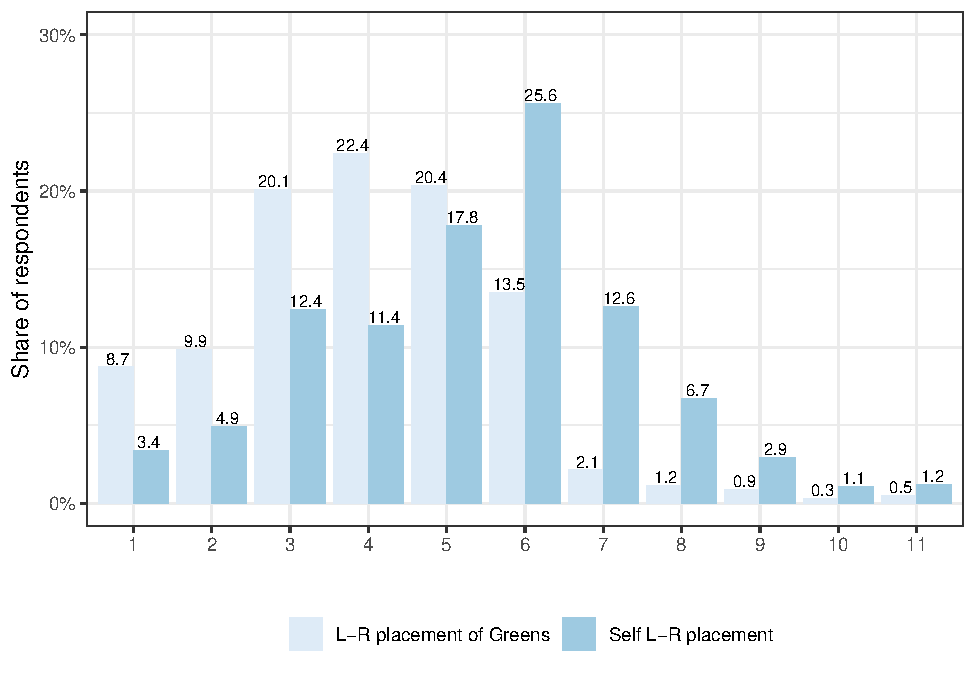
\includegraphics{AVCD_Final_Assignment-Edenhofer_files/figure-latex/gruene-spatial-1.pdf}

\hypertarget{socio-demographic-correlates-1}{%
\subsubsection{Socio-demographic
Correlates}\label{socio-demographic-correlates-1}}

\begin{Shaded}
\begin{Highlighting}[]
\NormalTok{gruene\_income }\OtherTok{\textless{}{-}} \FunctionTok{glm}\NormalTok{(gruene\_21 }\SpecialCharTok{\textasciitilde{}}\NormalTok{ household\_income }\SpecialCharTok{+}\NormalTok{ age }\SpecialCharTok{+}\NormalTok{ abitur\_factor }\SpecialCharTok{+}\NormalTok{ sex1 }\SpecialCharTok{+}\NormalTok{ urban\_rural\_factor }\SpecialCharTok{+}\NormalTok{ ostwest\_factor, }\AttributeTok{family =} \FunctionTok{binomial}\NormalTok{(}\AttributeTok{link =} \StringTok{"logit"}\NormalTok{), }\AttributeTok{data =}\NormalTok{ gles\_mod)}
\CommentTok{\# plot }
\FunctionTok{cplot}\NormalTok{(gruene\_income, }\AttributeTok{x =} \StringTok{"household\_income"}\NormalTok{, }\AttributeTok{draw =}\NormalTok{ F) }\SpecialCharTok{\%\textgreater{}\%}
  \FunctionTok{as\_tibble}\NormalTok{() }\SpecialCharTok{\%\textgreater{}\%}
   \FunctionTok{ggplot}\NormalTok{(}\FunctionTok{aes}\NormalTok{(}\AttributeTok{x =}\NormalTok{ xvals)) }\SpecialCharTok{+}
   \FunctionTok{geom\_line}\NormalTok{(}\FunctionTok{aes}\NormalTok{(}\AttributeTok{y =}\NormalTok{ yvals)) }\SpecialCharTok{+}
   \FunctionTok{geom\_ribbon}\NormalTok{(}\FunctionTok{aes}\NormalTok{(}\AttributeTok{ymin =}\NormalTok{ lower, }\AttributeTok{ymax =}\NormalTok{ upper), }\AttributeTok{alpha =} \FloatTok{0.2}\NormalTok{) }\SpecialCharTok{+} 
   \FunctionTok{scale\_x\_continuous}\NormalTok{(}\StringTok{"Net Monthly Household Income"}\NormalTok{,}
                     \AttributeTok{breaks =} \FunctionTok{seq}\NormalTok{(}\DecValTok{1}\NormalTok{, }\DecValTok{13}\NormalTok{, }\DecValTok{1}\NormalTok{),}
                     \AttributeTok{labels =} \FunctionTok{c}\NormalTok{(}\StringTok{"\textless{}500€"}\NormalTok{, }\StringTok{"[500{-}750€)"}\NormalTok{,}
                                \StringTok{"[750{-}1000€)"}\NormalTok{, }\StringTok{"[1000{-}1250€)"}\NormalTok{, }
                                \StringTok{"[1250{-}1500€)"}\NormalTok{, }\StringTok{"[1500{-}2000€)"}\NormalTok{,}
                                \StringTok{"[2000{-}2500€)"}\NormalTok{, }\StringTok{"[2500{-}3000€)"}\NormalTok{,}
                                \StringTok{"[3000{-}4000€)"}\NormalTok{, }\StringTok{"[4000{-}5000€)"}\NormalTok{,}
                                \StringTok{"[5000{-}7000€)"}\NormalTok{, }\StringTok{"[7000{-}10000€)"}\NormalTok{,}
                                \StringTok{"\textgreater{}10000€"}\NormalTok{)) }\SpecialCharTok{+}
  \FunctionTok{labs}\NormalTok{(}\AttributeTok{y =} \StringTok{"Predicted Probability of Voting Green"}\NormalTok{) }\SpecialCharTok{+}
  \FunctionTok{ylim}\NormalTok{(}\FunctionTok{c}\NormalTok{(}\DecValTok{0}\NormalTok{, }\FloatTok{0.2}\NormalTok{)) }\SpecialCharTok{+}
  \FunctionTok{theme\_bw}\NormalTok{() }\SpecialCharTok{+}
  \FunctionTok{theme}\NormalTok{(}\AttributeTok{axis.text.x =} \FunctionTok{element\_text}\NormalTok{(}\AttributeTok{angle =} \DecValTok{15}\NormalTok{, }\AttributeTok{hjust =} \DecValTok{1}\NormalTok{))}
\end{Highlighting}
\end{Shaded}

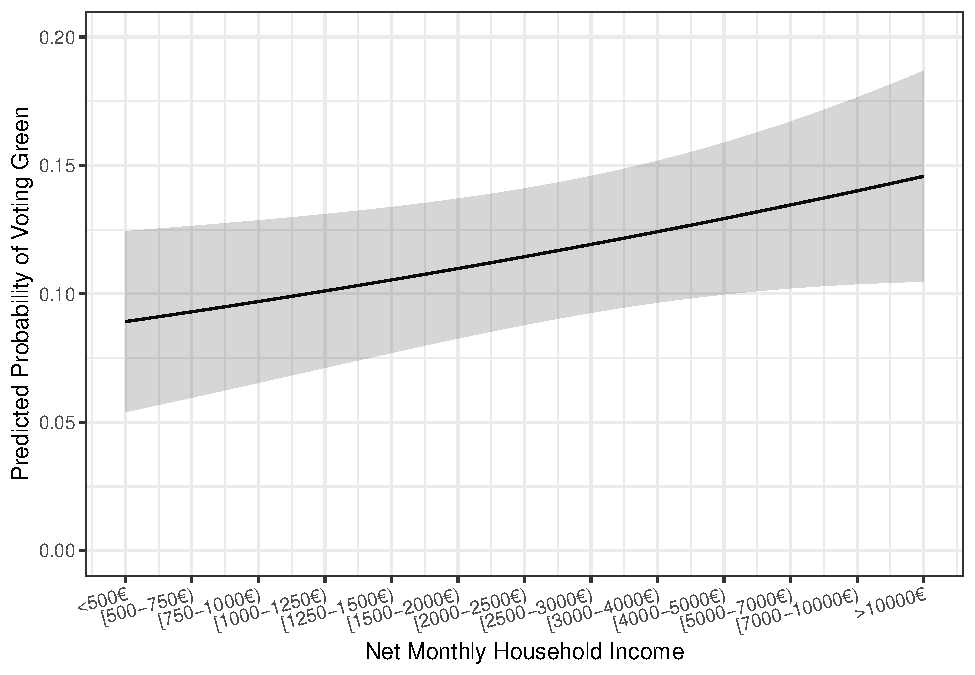
\includegraphics{AVCD_Final_Assignment-Edenhofer_files/figure-latex/gruene-income-1.pdf}

\begin{Shaded}
\begin{Highlighting}[]
\NormalTok{gruene\_sclass }\OtherTok{\textless{}{-}} \FunctionTok{glm}\NormalTok{(gruene\_21 }\SpecialCharTok{\textasciitilde{}}\NormalTok{ subjective\_class }\SpecialCharTok{+}\NormalTok{ age }\SpecialCharTok{+}\NormalTok{ abitur\_factor }\SpecialCharTok{+}\NormalTok{ sex1 }\SpecialCharTok{+}\NormalTok{ urban\_rural\_factor }\SpecialCharTok{+}\NormalTok{ ostwest\_factor, }\AttributeTok{family =} \FunctionTok{binomial}\NormalTok{(}\AttributeTok{link =} \StringTok{"logit"}\NormalTok{), }\AttributeTok{data =}\NormalTok{ gles\_mod)}
\CommentTok{\# plot }
\FunctionTok{cplot}\NormalTok{(gruene\_sclass, }\AttributeTok{x =} \StringTok{"subjective\_class"}\NormalTok{, }
      \AttributeTok{xvals =} \FunctionTok{seq}\NormalTok{(}\DecValTok{1}\NormalTok{, }\DecValTok{6}\NormalTok{, }\DecValTok{1}\NormalTok{),}
      \AttributeTok{draw =}\NormalTok{ F) }\SpecialCharTok{\%\textgreater{}\%}
  \FunctionTok{as\_tibble}\NormalTok{() }\SpecialCharTok{\%\textgreater{}\%}
  \FunctionTok{ggplot}\NormalTok{(}\FunctionTok{aes}\NormalTok{(}\AttributeTok{x =}\NormalTok{ xvals)) }\SpecialCharTok{+}
  \FunctionTok{geom\_point}\NormalTok{(}\FunctionTok{aes}\NormalTok{(}\AttributeTok{y =}\NormalTok{ yvals)) }\SpecialCharTok{+}
  \FunctionTok{geom\_errorbar}\NormalTok{(}\FunctionTok{aes}\NormalTok{(}\AttributeTok{ymin =}\NormalTok{ lower, }\AttributeTok{ymax =}\NormalTok{ upper), }\AttributeTok{width =} \FloatTok{0.2}\NormalTok{) }\SpecialCharTok{+}
  \FunctionTok{scale\_x\_continuous}\NormalTok{(}\StringTok{"Subjective Class"}\NormalTok{, }
                     \AttributeTok{breaks =} \FunctionTok{seq}\NormalTok{(}\DecValTok{1}\NormalTok{, }\DecValTok{6}\NormalTok{, }\DecValTok{1}\NormalTok{), }
                     \AttributeTok{labels =} \FunctionTok{c}\NormalTok{(}\StringTok{"Unterschicht"}\NormalTok{, }\StringTok{"Arbeiterschicht"}\NormalTok{, }
                                \StringTok{"Untere Mittelschicht"}\NormalTok{, }\StringTok{"mittlere Mittelschicht"}\NormalTok{, }\StringTok{"obere Mittelschicht"}\NormalTok{, }\StringTok{"Oberschicht"}\NormalTok{)) }\SpecialCharTok{+}
  \FunctionTok{labs}\NormalTok{(}\AttributeTok{y =} \StringTok{"Predicted Probability of Voting Green"}\NormalTok{) }\SpecialCharTok{+}
  \FunctionTok{ylim}\NormalTok{(}\FunctionTok{c}\NormalTok{(}\DecValTok{0}\NormalTok{, }\FloatTok{0.25}\NormalTok{)) }\SpecialCharTok{+}
  \FunctionTok{theme\_bw}\NormalTok{() }\SpecialCharTok{+}
  \FunctionTok{theme}\NormalTok{(}\AttributeTok{axis.text.x =} \FunctionTok{element\_text}\NormalTok{(}\AttributeTok{angle =} \DecValTok{15}\NormalTok{, }\AttributeTok{hjust =} \DecValTok{1}\NormalTok{))}
\end{Highlighting}
\end{Shaded}

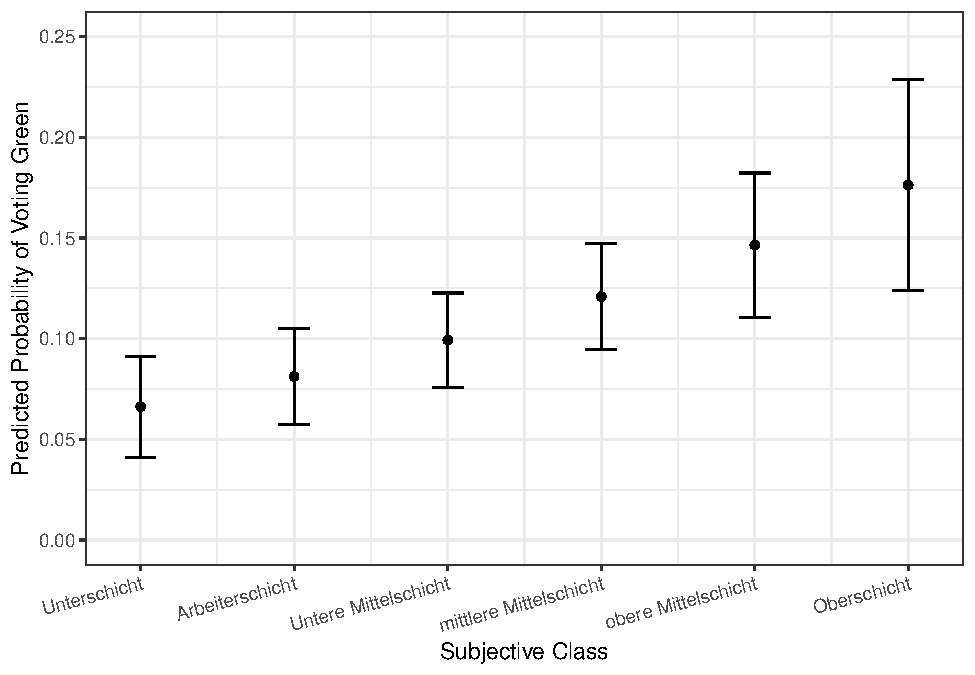
\includegraphics{AVCD_Final_Assignment-Edenhofer_files/figure-latex/gruene-subjective-class-1.pdf}

\begin{Shaded}
\begin{Highlighting}[]
\FunctionTok{cplot}\NormalTok{(gruene\_income, }\AttributeTok{x =} \StringTok{"urban\_rural\_factor"}\NormalTok{, }\AttributeTok{draw =}\NormalTok{ F) }\SpecialCharTok{\%\textgreater{}\%}
  \FunctionTok{as\_tibble}\NormalTok{() }\SpecialCharTok{\%\textgreater{}\%}
  \FunctionTok{ggplot}\NormalTok{(}\FunctionTok{aes}\NormalTok{(}\AttributeTok{x =}\NormalTok{ xvals)) }\SpecialCharTok{+}
  \FunctionTok{geom\_point}\NormalTok{(}\FunctionTok{aes}\NormalTok{(}\AttributeTok{y =}\NormalTok{ yvals)) }\SpecialCharTok{+}
  \FunctionTok{geom\_errorbar}\NormalTok{(}\FunctionTok{aes}\NormalTok{(}\AttributeTok{ymin =}\NormalTok{ lower, }\AttributeTok{ymax =}\NormalTok{ upper), }\AttributeTok{width =} \FloatTok{0.2}\NormalTok{) }\SpecialCharTok{+}
  \FunctionTok{scale\_x\_discrete}\NormalTok{(}\StringTok{"Urban{-}Rural"}\NormalTok{, }
                   \AttributeTok{labels =} \FunctionTok{c}\NormalTok{(}\StringTok{"Grossstadt"}\NormalTok{, }\StringTok{"Rand/Vorort grosser Stadt"}\NormalTok{,}
                              \StringTok{"Mittel{-}oder Kleinstadt"}\NormalTok{, }\StringTok{"laendliches Dorf"}\NormalTok{,}
                              \StringTok{"Einzelgehoeft"}\NormalTok{)) }\SpecialCharTok{+}
 \FunctionTok{labs}\NormalTok{(}\AttributeTok{y =} \StringTok{"Predicted Probability of Voting Green"}\NormalTok{) }\SpecialCharTok{+}
 \FunctionTok{ylim}\NormalTok{(}\FunctionTok{c}\NormalTok{(}\DecValTok{0}\NormalTok{, }\FloatTok{0.25}\NormalTok{)) }\SpecialCharTok{+}
 \FunctionTok{theme\_bw}\NormalTok{() }\SpecialCharTok{+}
 \FunctionTok{theme}\NormalTok{(}\AttributeTok{axis.text.x =} \FunctionTok{element\_text}\NormalTok{(}\AttributeTok{angle =} \DecValTok{15}\NormalTok{, }\AttributeTok{hjust =} \DecValTok{1}\NormalTok{))}
\end{Highlighting}
\end{Shaded}

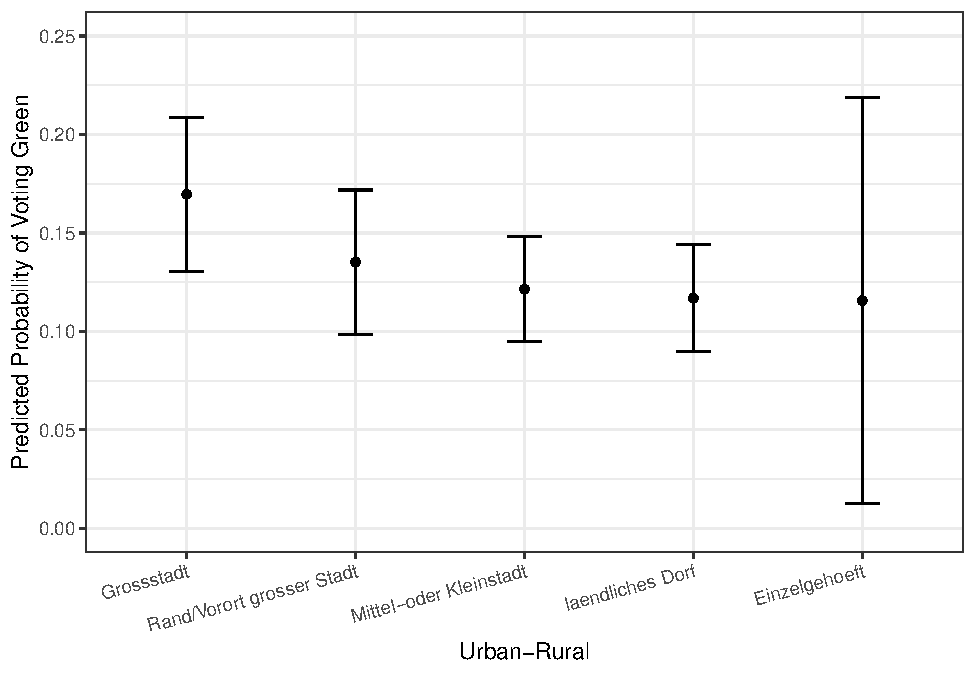
\includegraphics{AVCD_Final_Assignment-Edenhofer_files/figure-latex/gruene-geography-1.pdf}

\begin{Shaded}
\begin{Highlighting}[]
\CommentTok{\# plot }
\FunctionTok{cplot}\NormalTok{(gruene\_income,}
       \AttributeTok{x =} \StringTok{"age"}\NormalTok{, }\AttributeTok{draw =}\NormalTok{ F) }\SpecialCharTok{\%\textgreater{}\%}
   \FunctionTok{as\_tibble}\NormalTok{() }\SpecialCharTok{\%\textgreater{}\%}
   \FunctionTok{ggplot}\NormalTok{(}\FunctionTok{aes}\NormalTok{(}\AttributeTok{x =}\NormalTok{ xvals)) }\SpecialCharTok{+}
   \FunctionTok{geom\_line}\NormalTok{(}\FunctionTok{aes}\NormalTok{(}\AttributeTok{y =}\NormalTok{ yvals)) }\SpecialCharTok{+}
   \FunctionTok{geom\_ribbon}\NormalTok{(}\FunctionTok{aes}\NormalTok{(}\AttributeTok{ymin =}\NormalTok{ lower, }\AttributeTok{ymax =}\NormalTok{ upper), }\AttributeTok{alpha =} \FloatTok{0.2}\NormalTok{) }\SpecialCharTok{+}
   \FunctionTok{scale\_x\_continuous}\NormalTok{(}\StringTok{"Age"}\NormalTok{, }\AttributeTok{breaks =} \FunctionTok{seq}\NormalTok{(}\DecValTok{20}\NormalTok{, }\DecValTok{90}\NormalTok{, }\DecValTok{10}\NormalTok{)) }\SpecialCharTok{+}
   \FunctionTok{ylim}\NormalTok{(}\FunctionTok{c}\NormalTok{(}\DecValTok{0}\NormalTok{, }\FloatTok{0.4}\NormalTok{)) }\SpecialCharTok{+}
   \FunctionTok{theme\_bw}\NormalTok{()  }
\end{Highlighting}
\end{Shaded}

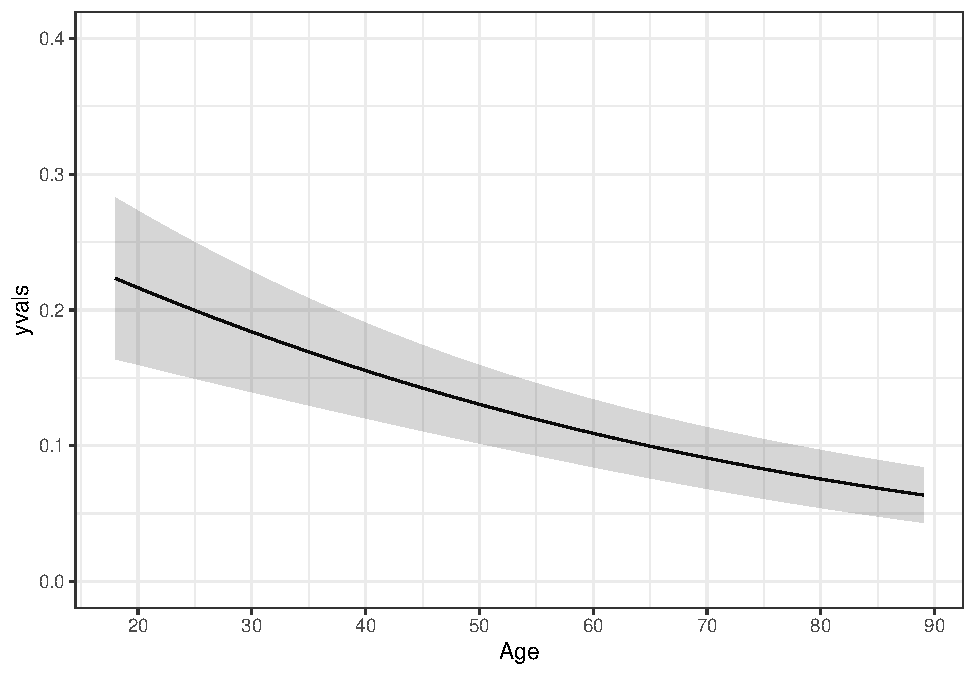
\includegraphics{AVCD_Final_Assignment-Edenhofer_files/figure-latex/gruene-age-1.pdf}

\begin{Shaded}
\begin{Highlighting}[]
\NormalTok{gruene\_left\_right\_self }\OtherTok{\textless{}{-}} \FunctionTok{glm}\NormalTok{(gruene\_21 }\SpecialCharTok{\textasciitilde{}}\NormalTok{ left\_right\_self }\SpecialCharTok{+} \FunctionTok{I}\NormalTok{(left\_right\_self}\SpecialCharTok{\^{}}\DecValTok{2}\NormalTok{) }\SpecialCharTok{+}\NormalTok{ age }\SpecialCharTok{+}\NormalTok{ abitur\_factor }\SpecialCharTok{+}\NormalTok{ sex1 }\SpecialCharTok{+}\NormalTok{ urban\_rural\_factor }\SpecialCharTok{+}\NormalTok{ ostwest\_factor, }\AttributeTok{family =} \FunctionTok{binomial}\NormalTok{(}\AttributeTok{link =} \StringTok{"logit"}\NormalTok{), }\AttributeTok{data =}\NormalTok{ gles\_mod)}
\CommentTok{\# plot }
\FunctionTok{cplot}\NormalTok{(gruene\_left\_right\_self, }\AttributeTok{x =} \StringTok{"left\_right\_self"}\NormalTok{, }
      \AttributeTok{xvals =} \FunctionTok{seq}\NormalTok{(}\DecValTok{1}\NormalTok{, }\DecValTok{11}\NormalTok{, }\DecValTok{1}\NormalTok{),}
      \AttributeTok{draw =}\NormalTok{ F) }\SpecialCharTok{\%\textgreater{}\%}
  \FunctionTok{as\_tibble}\NormalTok{() }\SpecialCharTok{\%\textgreater{}\%}
  \FunctionTok{ggplot}\NormalTok{(}\FunctionTok{aes}\NormalTok{(}\AttributeTok{x =}\NormalTok{ xvals)) }\SpecialCharTok{+}
  \FunctionTok{geom\_point}\NormalTok{(}\FunctionTok{aes}\NormalTok{(}\AttributeTok{y =}\NormalTok{ yvals)) }\SpecialCharTok{+}
  \FunctionTok{geom\_errorbar}\NormalTok{(}\FunctionTok{aes}\NormalTok{(}\AttributeTok{ymin =}\NormalTok{ lower, }\AttributeTok{ymax =}\NormalTok{ upper), }\AttributeTok{width =} \FloatTok{0.2}\NormalTok{) }\SpecialCharTok{+}
  \FunctionTok{scale\_x\_continuous}\NormalTok{(}\StringTok{"Left{-}Right Self{-}Placement"}\NormalTok{, }
                     \AttributeTok{breaks =} \FunctionTok{seq}\NormalTok{(}\DecValTok{1}\NormalTok{, }\DecValTok{11}\NormalTok{, }\DecValTok{1}\NormalTok{)) }\SpecialCharTok{+}
  \FunctionTok{labs}\NormalTok{(}\AttributeTok{y =} \StringTok{"Predicted Probability of Voting Green"}\NormalTok{) }\SpecialCharTok{+}
  \FunctionTok{theme\_bw}\NormalTok{()}
\end{Highlighting}
\end{Shaded}

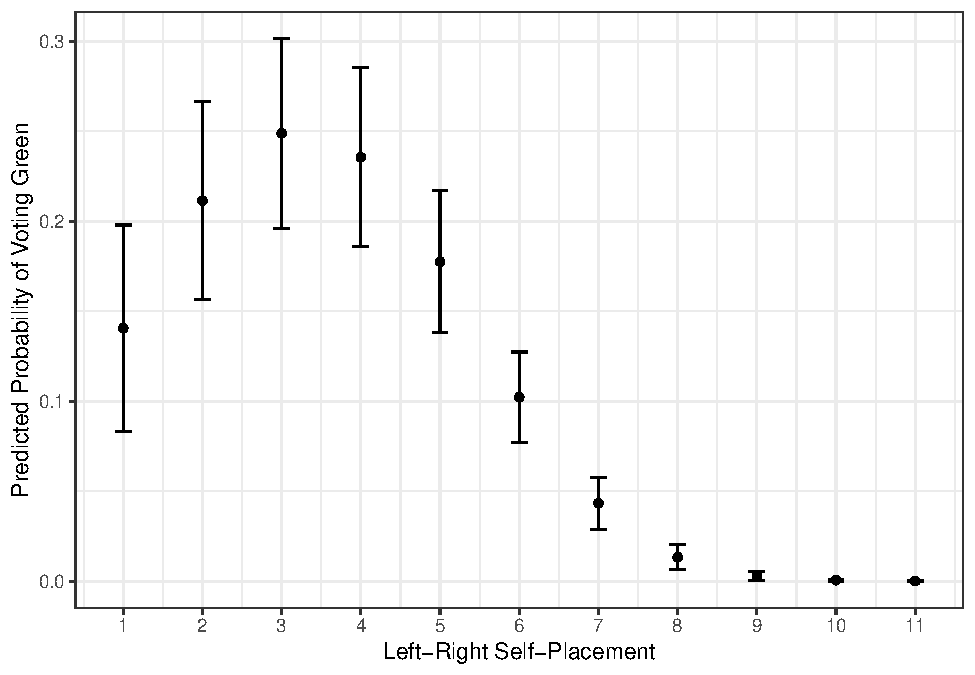
\includegraphics{AVCD_Final_Assignment-Edenhofer_files/figure-latex/gruene-left-right-self-placement-1.pdf}

\begin{Shaded}
\begin{Highlighting}[]
\FunctionTok{cplot}\NormalTok{(gruene\_income, }\AttributeTok{x =} \StringTok{"abitur\_factor"}\NormalTok{, }\AttributeTok{draw =}\NormalTok{ F) }\SpecialCharTok{\%\textgreater{}\%}
  \FunctionTok{as\_tibble}\NormalTok{() }\SpecialCharTok{\%\textgreater{}\%}
  \FunctionTok{ggplot}\NormalTok{(}\FunctionTok{aes}\NormalTok{(}\AttributeTok{x =}\NormalTok{ xvals)) }\SpecialCharTok{+}
  \FunctionTok{geom\_point}\NormalTok{(}\FunctionTok{aes}\NormalTok{(}\AttributeTok{y =}\NormalTok{ yvals)) }\SpecialCharTok{+}
  \FunctionTok{geom\_errorbar}\NormalTok{(}\FunctionTok{aes}\NormalTok{(}\AttributeTok{ymin =}\NormalTok{ lower, }\AttributeTok{ymax =}\NormalTok{ upper), }\AttributeTok{width =} \FloatTok{0.2}\NormalTok{) }\SpecialCharTok{+}
  \FunctionTok{scale\_x\_discrete}\NormalTok{(}\StringTok{"Education"}\NormalTok{, }\AttributeTok{labels =} \FunctionTok{c}\NormalTok{(}\StringTok{"At Least Abitur"}\NormalTok{, }
                                           \StringTok{"No Abitur"}\NormalTok{)) }\SpecialCharTok{+}
  \FunctionTok{labs}\NormalTok{(}\AttributeTok{y =} \StringTok{"Predicted Probability of Voting Green"}\NormalTok{, }
       \AttributeTok{caption =} \StringTok{"Covariates include: age, household income, sex, rurality of place of residence and an east{-}west dummy."}\NormalTok{) }\SpecialCharTok{+}
  \FunctionTok{ylim}\NormalTok{(}\FunctionTok{c}\NormalTok{(}\FloatTok{0.05}\NormalTok{, }\FloatTok{0.3}\NormalTok{)) }\SpecialCharTok{+}
  \FunctionTok{theme\_bw}\NormalTok{()}
\end{Highlighting}
\end{Shaded}

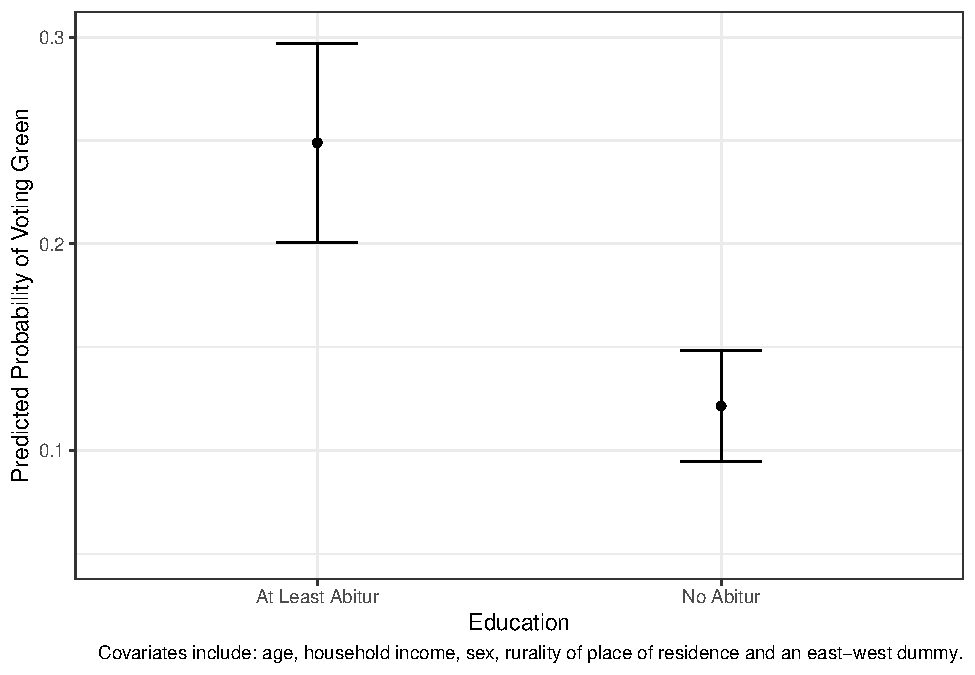
\includegraphics{AVCD_Final_Assignment-Edenhofer_files/figure-latex/gruene-education-1.pdf}

\begin{Shaded}
\begin{Highlighting}[]
\FunctionTok{cplot}\NormalTok{(gruene\_income, }\AttributeTok{x =} \StringTok{"ostwest\_factor"}\NormalTok{, }\AttributeTok{draw =}\NormalTok{ F) }\SpecialCharTok{\%\textgreater{}\%}
  \FunctionTok{as\_tibble}\NormalTok{() }\SpecialCharTok{\%\textgreater{}\%}
  \FunctionTok{ggplot}\NormalTok{(}\FunctionTok{aes}\NormalTok{(}\AttributeTok{x =}\NormalTok{ xvals)) }\SpecialCharTok{+}
  \FunctionTok{geom\_point}\NormalTok{(}\FunctionTok{aes}\NormalTok{(}\AttributeTok{y =}\NormalTok{ yvals)) }\SpecialCharTok{+}
  \FunctionTok{geom\_errorbar}\NormalTok{(}\FunctionTok{aes}\NormalTok{(}\AttributeTok{ymin =}\NormalTok{ lower, }\AttributeTok{ymax =}\NormalTok{ upper), }\AttributeTok{width =} \FloatTok{0.2}\NormalTok{) }\SpecialCharTok{+}
  \FunctionTok{scale\_x\_discrete}\NormalTok{(}\StringTok{"Ost{-}West Dummy"}\NormalTok{, }\AttributeTok{labels =} \FunctionTok{c}\NormalTok{(}\StringTok{"Ost"}\NormalTok{, }\StringTok{"West"}\NormalTok{)) }\SpecialCharTok{+}
  \FunctionTok{ylim}\NormalTok{(}\FunctionTok{c}\NormalTok{(}\DecValTok{0}\NormalTok{, }\FloatTok{0.2}\NormalTok{)) }\SpecialCharTok{+}
  \FunctionTok{labs}\NormalTok{(}\AttributeTok{y =} \StringTok{"Predicted Probability of Voting Gruene"}\NormalTok{) }\SpecialCharTok{+}
  \FunctionTok{theme\_bw}\NormalTok{()}
\end{Highlighting}
\end{Shaded}

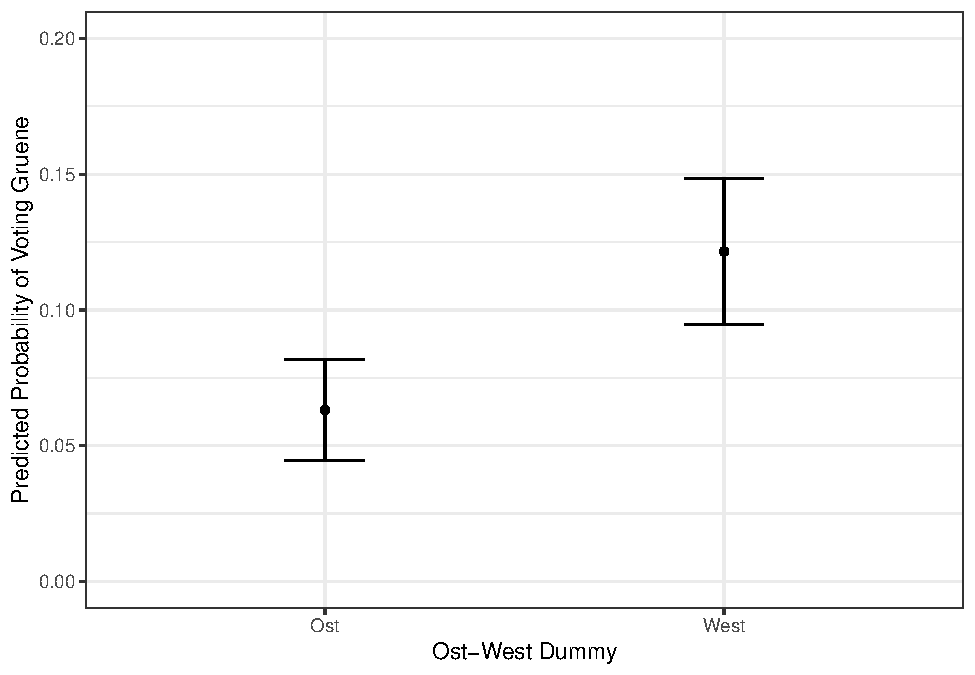
\includegraphics{AVCD_Final_Assignment-Edenhofer_files/figure-latex/gruene-ost-west-1.pdf}

\hypertarget{attiudinal-correlates-1}{%
\subsubsection{Attiudinal Correlates}\label{attiudinal-correlates-1}}

\begin{Shaded}
\begin{Highlighting}[]
\NormalTok{gruene\_cancel }\OtherTok{\textless{}{-}} \FunctionTok{glm}\NormalTok{(gruene\_21 }\SpecialCharTok{\textasciitilde{}}\NormalTok{ cancel\_culture\_subjektiv }\SpecialCharTok{+}\NormalTok{ household\_income }\SpecialCharTok{+}\NormalTok{ age }\SpecialCharTok{+}\NormalTok{ abitur\_factor }\SpecialCharTok{+}\NormalTok{ sex1 }\SpecialCharTok{+}\NormalTok{ urban\_rural\_factor }\SpecialCharTok{+}\NormalTok{ ostwest\_factor, }\AttributeTok{family =} \FunctionTok{binomial}\NormalTok{(}\AttributeTok{link =} \StringTok{"logit"}\NormalTok{), }\AttributeTok{data =}\NormalTok{ gles\_mod)}
\CommentTok{\# plot}
\FunctionTok{cplot}\NormalTok{(gruene\_cancel, }\AttributeTok{x =} \StringTok{"cancel\_culture\_subjektiv"}\NormalTok{, }
      \AttributeTok{xvals =} \FunctionTok{seq}\NormalTok{(}\DecValTok{1}\NormalTok{, }\DecValTok{5}\NormalTok{, }\DecValTok{1}\NormalTok{), }\AttributeTok{draw =}\NormalTok{ F) }\SpecialCharTok{\%\textgreater{}\%}
  \FunctionTok{as\_tibble}\NormalTok{() }\SpecialCharTok{\%\textgreater{}\%}
  \FunctionTok{ggplot}\NormalTok{(}\FunctionTok{aes}\NormalTok{(}\AttributeTok{x =}\NormalTok{ xvals)) }\SpecialCharTok{+}
  \FunctionTok{geom\_point}\NormalTok{(}\FunctionTok{aes}\NormalTok{(}\AttributeTok{y =}\NormalTok{ yvals)) }\SpecialCharTok{+}
  \FunctionTok{geom\_errorbar}\NormalTok{(}\FunctionTok{aes}\NormalTok{(}\AttributeTok{ymin =}\NormalTok{ lower, }\AttributeTok{ymax =}\NormalTok{ upper), }\AttributeTok{width =} \FloatTok{0.2}\NormalTok{) }\SpecialCharTok{+}
  \FunctionTok{scale\_x\_continuous}\NormalTok{(}\StringTok{"Subjektiv: Keine freie Meinungsaeusserung moeglich"}\NormalTok{, }
                   \AttributeTok{breaks =} \FunctionTok{seq}\NormalTok{(}\DecValTok{1}\NormalTok{, }\DecValTok{5}\NormalTok{, }\DecValTok{1}\NormalTok{),}
                   \AttributeTok{labels =} \FunctionTok{c}\NormalTok{(}\StringTok{"Stimme voll zu"}\NormalTok{, }\StringTok{"Stimme eher zu"}\NormalTok{,}
                              \StringTok{"Teils/Teils"}\NormalTok{, }\StringTok{"Stimme eher nicht zu"}\NormalTok{,}
                              \StringTok{"Stimme ueberhaupt nicht zu"}\NormalTok{)) }\SpecialCharTok{+}
  \FunctionTok{labs}\NormalTok{(}\AttributeTok{y =} \StringTok{"Predicted Probability of Voting Green"}\NormalTok{) }\SpecialCharTok{+}
  \FunctionTok{ylim}\NormalTok{(}\FunctionTok{c}\NormalTok{(}\DecValTok{0}\NormalTok{, }\FloatTok{0.3}\NormalTok{)) }\SpecialCharTok{+}
  \FunctionTok{theme\_bw}\NormalTok{() }\SpecialCharTok{+}
  \FunctionTok{theme}\NormalTok{(}\AttributeTok{axis.text.x =} \FunctionTok{element\_text}\NormalTok{(}\AttributeTok{angle =} \DecValTok{15}\NormalTok{, }\AttributeTok{hjust =} \DecValTok{1}\NormalTok{))}
\end{Highlighting}
\end{Shaded}

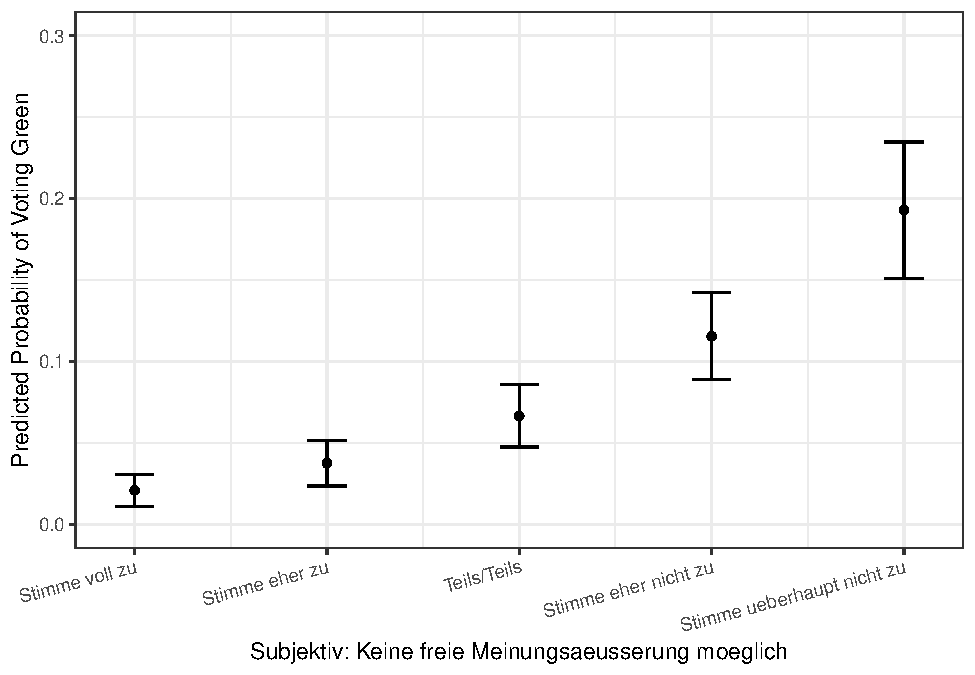
\includegraphics{AVCD_Final_Assignment-Edenhofer_files/figure-latex/gruene-cancel-culture-1.pdf}

\begin{Shaded}
\begin{Highlighting}[]
\NormalTok{gruene\_trust\_parliament }\OtherTok{\textless{}{-}} \FunctionTok{glm}\NormalTok{(gruene\_21 }\SpecialCharTok{\textasciitilde{}}\NormalTok{ trust\_in\_parliament }\SpecialCharTok{+} \FunctionTok{I}\NormalTok{(trust\_in\_parliament}\SpecialCharTok{\^{}}\DecValTok{2}\NormalTok{) }\SpecialCharTok{+}\NormalTok{ household\_income }\SpecialCharTok{+}\NormalTok{ age }\SpecialCharTok{+}\NormalTok{ abitur\_factor }\SpecialCharTok{+}\NormalTok{ sex1 }\SpecialCharTok{+}\NormalTok{ urban\_rural\_factor }\SpecialCharTok{+}\NormalTok{ ostwest\_factor, }\AttributeTok{family =} \FunctionTok{binomial}\NormalTok{(}\AttributeTok{link =} \StringTok{"logit"}\NormalTok{), }\AttributeTok{data =}\NormalTok{ gles\_mod)}
\CommentTok{\# plot}
\FunctionTok{cplot}\NormalTok{(gruene\_trust\_parliament, }\AttributeTok{x =} \StringTok{"trust\_in\_parliament"}\NormalTok{, }
      \AttributeTok{xvals =} \FunctionTok{seq}\NormalTok{(}\DecValTok{1}\NormalTok{, }\DecValTok{11}\NormalTok{, }\DecValTok{1}\NormalTok{), }\AttributeTok{draw =}\NormalTok{ F) }\SpecialCharTok{\%\textgreater{}\%}
  \FunctionTok{as\_tibble}\NormalTok{() }\SpecialCharTok{\%\textgreater{}\%}
  \FunctionTok{ggplot}\NormalTok{(}\FunctionTok{aes}\NormalTok{(}\AttributeTok{x =}\NormalTok{ xvals)) }\SpecialCharTok{+}
  \FunctionTok{geom\_point}\NormalTok{(}\FunctionTok{aes}\NormalTok{(}\AttributeTok{y =}\NormalTok{ yvals)) }\SpecialCharTok{+}
  \FunctionTok{geom\_errorbar}\NormalTok{(}\FunctionTok{aes}\NormalTok{(}\AttributeTok{ymin =}\NormalTok{ lower, }\AttributeTok{ymax =}\NormalTok{ upper), }\AttributeTok{width =} \FloatTok{0.2}\NormalTok{) }\SpecialCharTok{+}
  \FunctionTok{scale\_x\_continuous}\NormalTok{(}\StringTok{"Vertrauen: Bundestag"}\NormalTok{, }
                     \AttributeTok{breaks =} \FunctionTok{seq}\NormalTok{(}\DecValTok{1}\NormalTok{, }\DecValTok{11}\NormalTok{, }\DecValTok{1}\NormalTok{)) }\SpecialCharTok{+}
  \FunctionTok{labs}\NormalTok{(}\AttributeTok{y =} \StringTok{"Predicted Probability of Voting Green"}\NormalTok{, }
       \AttributeTok{caption =} \StringTok{"\textquotesingle{}1\textquotesingle{} indicates \textquotesingle{}no trust\textquotesingle{}, while 11 indicates \textquotesingle{}full trust\textquotesingle{}."}\NormalTok{) }\SpecialCharTok{+}
  \FunctionTok{ylim}\NormalTok{(}\FunctionTok{c}\NormalTok{(}\DecValTok{0}\NormalTok{, }\FloatTok{0.3}\NormalTok{)) }\SpecialCharTok{+}
  \FunctionTok{theme\_bw}\NormalTok{()}
\end{Highlighting}
\end{Shaded}

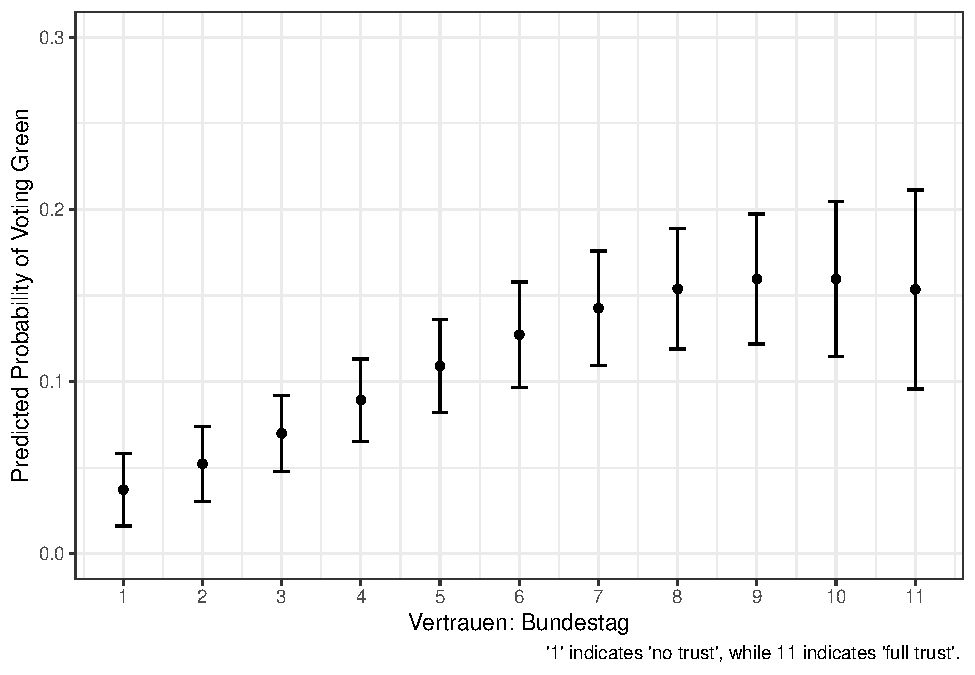
\includegraphics{AVCD_Final_Assignment-Edenhofer_files/figure-latex/gruene-trust-parliament-1.pdf}

\begin{Shaded}
\begin{Highlighting}[]
\NormalTok{gruene\_trust\_parties }\OtherTok{\textless{}{-}} \FunctionTok{glm}\NormalTok{(gruene\_21 }\SpecialCharTok{\textasciitilde{}}\NormalTok{ trust\_in\_parties }\SpecialCharTok{+} \FunctionTok{I}\NormalTok{(trust\_in\_parties}\SpecialCharTok{\^{}}\DecValTok{2}\NormalTok{) }\SpecialCharTok{+}\NormalTok{ household\_income }\SpecialCharTok{+}\NormalTok{ age }\SpecialCharTok{+}\NormalTok{ abitur\_factor }\SpecialCharTok{+}\NormalTok{ sex1 }\SpecialCharTok{+}\NormalTok{ urban\_rural\_factor }\SpecialCharTok{+}\NormalTok{ ostwest\_factor, }\AttributeTok{family =} \FunctionTok{binomial}\NormalTok{(}\AttributeTok{link =} \StringTok{"logit"}\NormalTok{), }\AttributeTok{data =}\NormalTok{ gles\_mod)}
\CommentTok{\# plot}
\FunctionTok{cplot}\NormalTok{(gruene\_trust\_parties, }\AttributeTok{x =} \StringTok{"trust\_in\_parties"}\NormalTok{,}
      \AttributeTok{xvals =} \FunctionTok{seq}\NormalTok{(}\DecValTok{1}\NormalTok{, }\DecValTok{11}\NormalTok{, }\DecValTok{1}\NormalTok{), }\AttributeTok{draw =}\NormalTok{ F) }\SpecialCharTok{\%\textgreater{}\%}
  \FunctionTok{as\_tibble}\NormalTok{() }\SpecialCharTok{\%\textgreater{}\%}
  \FunctionTok{ggplot}\NormalTok{(}\FunctionTok{aes}\NormalTok{(}\AttributeTok{x =}\NormalTok{ xvals)) }\SpecialCharTok{+}
  \FunctionTok{geom\_point}\NormalTok{(}\FunctionTok{aes}\NormalTok{(}\AttributeTok{y =}\NormalTok{ yvals)) }\SpecialCharTok{+}
  \FunctionTok{geom\_errorbar}\NormalTok{(}\FunctionTok{aes}\NormalTok{(}\AttributeTok{ymin =}\NormalTok{ lower, }\AttributeTok{ymax =}\NormalTok{ upper), }\AttributeTok{width =} \FloatTok{0.2}\NormalTok{) }\SpecialCharTok{+}
  \FunctionTok{scale\_x\_continuous}\NormalTok{(}\StringTok{"Vertrauen: Parteien"}\NormalTok{, }
                     \AttributeTok{breaks =} \FunctionTok{seq}\NormalTok{(}\DecValTok{1}\NormalTok{, }\DecValTok{11}\NormalTok{, }\DecValTok{1}\NormalTok{)) }\SpecialCharTok{+}
  \FunctionTok{labs}\NormalTok{(}\AttributeTok{y =} \StringTok{"Predicted Probability of Voting Green"}\NormalTok{, }
       \AttributeTok{caption =} \StringTok{"\textquotesingle{}1\textquotesingle{} indicates \textquotesingle{}no trust\textquotesingle{}, while 11 indicates \textquotesingle{}full trust\textquotesingle{}."}\NormalTok{) }\SpecialCharTok{+}
  \FunctionTok{ylim}\NormalTok{(}\FunctionTok{c}\NormalTok{(}\DecValTok{0}\NormalTok{, }\FloatTok{0.3}\NormalTok{)) }\SpecialCharTok{+}
  \FunctionTok{theme\_bw}\NormalTok{()}
\end{Highlighting}
\end{Shaded}

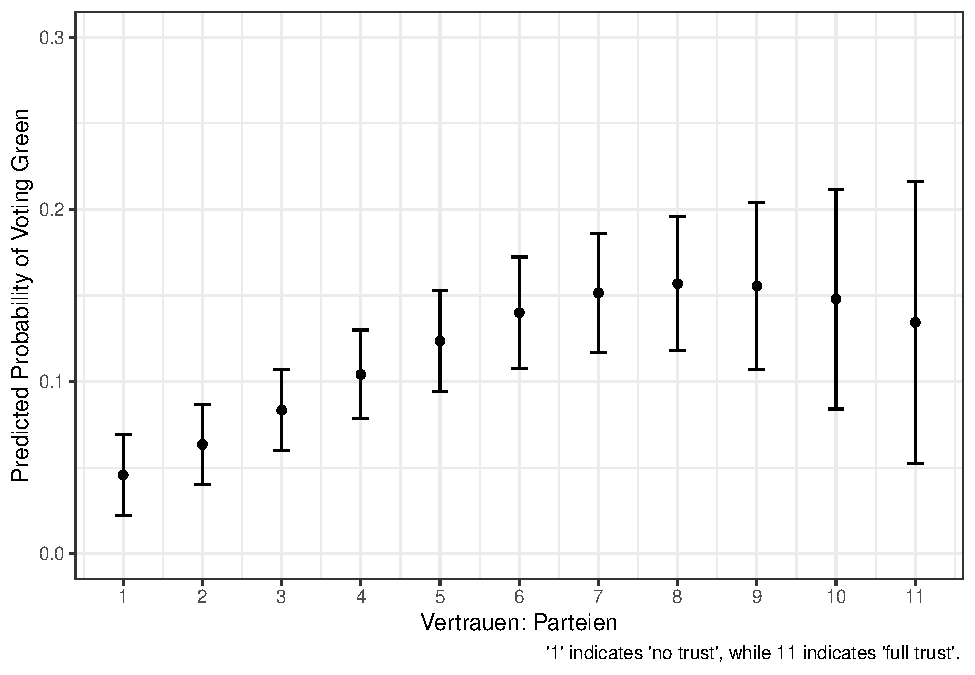
\includegraphics{AVCD_Final_Assignment-Edenhofer_files/figure-latex/gruene-trust-parties-1.pdf}

\begin{Shaded}
\begin{Highlighting}[]
\NormalTok{gruene\_trust\_politicians }\OtherTok{\textless{}{-}} \FunctionTok{glm}\NormalTok{(gruene\_21 }\SpecialCharTok{\textasciitilde{}}\NormalTok{ trust\_in\_politicians }\SpecialCharTok{+} \FunctionTok{I}\NormalTok{(trust\_in\_politicians}\SpecialCharTok{\^{}}\DecValTok{2}\NormalTok{) }\SpecialCharTok{+}\NormalTok{ household\_income }\SpecialCharTok{+}\NormalTok{ age }\SpecialCharTok{+}\NormalTok{ abitur\_factor }\SpecialCharTok{+}\NormalTok{ sex1 }\SpecialCharTok{+}\NormalTok{ urban\_rural\_factor }\SpecialCharTok{+}\NormalTok{ ostwest\_factor, }\AttributeTok{family =} \FunctionTok{binomial}\NormalTok{(}\AttributeTok{link =} \StringTok{"logit"}\NormalTok{), }\AttributeTok{data =}\NormalTok{ gles\_mod)}
\CommentTok{\# plot }
\FunctionTok{cplot}\NormalTok{(gruene\_trust\_politicians, }\AttributeTok{x =} \StringTok{"trust\_in\_politicians"}\NormalTok{,}
      \AttributeTok{xvals =} \FunctionTok{seq}\NormalTok{(}\DecValTok{1}\NormalTok{, }\DecValTok{11}\NormalTok{, }\DecValTok{1}\NormalTok{), }\AttributeTok{draw =}\NormalTok{ F) }\SpecialCharTok{\%\textgreater{}\%}
  \FunctionTok{as\_tibble}\NormalTok{() }\SpecialCharTok{\%\textgreater{}\%}
  \FunctionTok{ggplot}\NormalTok{(}\FunctionTok{aes}\NormalTok{(}\AttributeTok{x =}\NormalTok{ xvals)) }\SpecialCharTok{+}
  \FunctionTok{geom\_point}\NormalTok{(}\FunctionTok{aes}\NormalTok{(}\AttributeTok{y =}\NormalTok{ yvals)) }\SpecialCharTok{+}
  \FunctionTok{geom\_errorbar}\NormalTok{(}\FunctionTok{aes}\NormalTok{(}\AttributeTok{ymin =}\NormalTok{ lower, }\AttributeTok{ymax =}\NormalTok{ upper), }\AttributeTok{width =} \FloatTok{0.2}\NormalTok{) }\SpecialCharTok{+}
  \FunctionTok{scale\_x\_continuous}\NormalTok{(}\StringTok{"Vertrauen: Politiker:innen"}\NormalTok{, }
                     \AttributeTok{breaks =} \FunctionTok{seq}\NormalTok{(}\DecValTok{1}\NormalTok{, }\DecValTok{11}\NormalTok{, }\DecValTok{1}\NormalTok{)) }\SpecialCharTok{+}
  \FunctionTok{labs}\NormalTok{(}\AttributeTok{y =} \StringTok{"Predicted Probability of Voting Green"}\NormalTok{, }
       \AttributeTok{caption =} \StringTok{"\textquotesingle{}1\textquotesingle{} indicates \textquotesingle{}no trust\textquotesingle{}, while 11 indicates \textquotesingle{}full trust\textquotesingle{}."}\NormalTok{) }\SpecialCharTok{+}
  \FunctionTok{ylim}\NormalTok{(}\FunctionTok{c}\NormalTok{(}\DecValTok{0}\NormalTok{, }\FloatTok{0.3}\NormalTok{)) }\SpecialCharTok{+}
  \FunctionTok{theme\_bw}\NormalTok{()}
\end{Highlighting}
\end{Shaded}

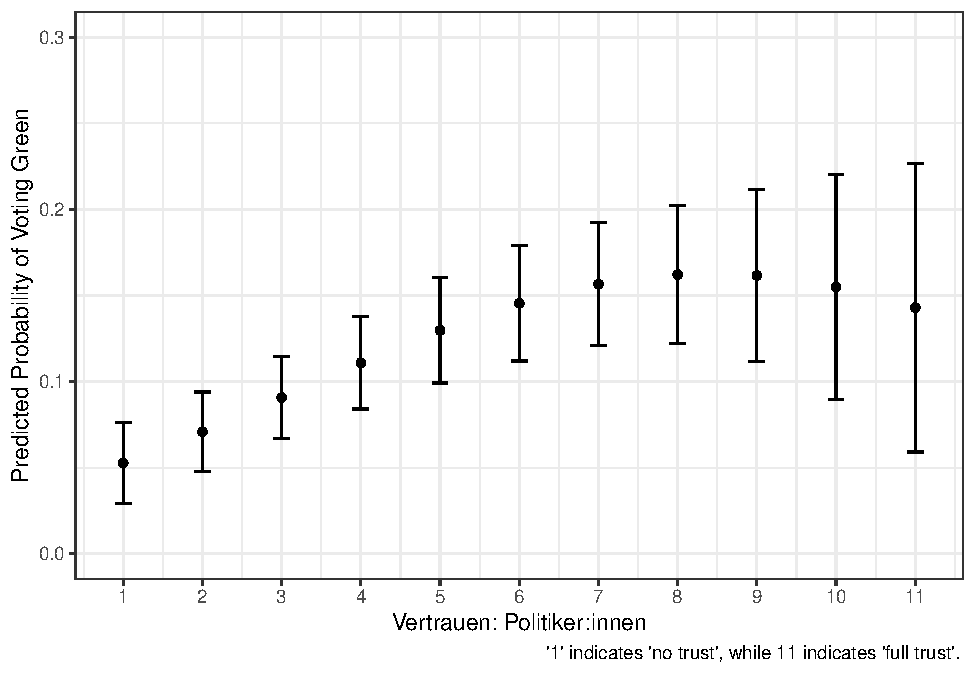
\includegraphics{AVCD_Final_Assignment-Edenhofer_files/figure-latex/gruene-trust-politicians-1.pdf}

\begin{Shaded}
\begin{Highlighting}[]
\NormalTok{gruene\_immig\_culture\_threat }\OtherTok{\textless{}{-}} \FunctionTok{glm}\NormalTok{(gruene\_21 }\SpecialCharTok{\textasciitilde{}}\NormalTok{ out\_group\_immig\_culture\_threat }\SpecialCharTok{+}\NormalTok{ household\_income }\SpecialCharTok{+}\NormalTok{ age }\SpecialCharTok{+}\NormalTok{ abitur\_factor }\SpecialCharTok{+}\NormalTok{ sex1 }\SpecialCharTok{+}\NormalTok{ urban\_rural\_factor }\SpecialCharTok{+}\NormalTok{ ostwest\_factor, }\AttributeTok{family =} \FunctionTok{binomial}\NormalTok{(}\AttributeTok{link =} \StringTok{"logit"}\NormalTok{), }\AttributeTok{data =}\NormalTok{ gles\_mod)}
\CommentTok{\# plot }
\FunctionTok{cplot}\NormalTok{(gruene\_immig\_culture\_threat, }\AttributeTok{x =} \StringTok{"out\_group\_immig\_culture\_threat"}\NormalTok{,}
      \AttributeTok{xvals =} \FunctionTok{seq}\NormalTok{(}\DecValTok{1}\NormalTok{, }\DecValTok{5}\NormalTok{, }\DecValTok{1}\NormalTok{), }\AttributeTok{draw =}\NormalTok{ F) }\SpecialCharTok{\%\textgreater{}\%}
  \FunctionTok{as\_tibble}\NormalTok{() }\SpecialCharTok{\%\textgreater{}\%}
  \FunctionTok{ggplot}\NormalTok{(}\FunctionTok{aes}\NormalTok{(}\AttributeTok{x =}\NormalTok{ xvals)) }\SpecialCharTok{+}
  \FunctionTok{geom\_point}\NormalTok{(}\FunctionTok{aes}\NormalTok{(}\AttributeTok{y =}\NormalTok{ yvals)) }\SpecialCharTok{+}
  \FunctionTok{geom\_errorbar}\NormalTok{(}\FunctionTok{aes}\NormalTok{(}\AttributeTok{ymin =}\NormalTok{ lower, }\AttributeTok{ymax =}\NormalTok{ upper), }\AttributeTok{width =} \FloatTok{0.2}\NormalTok{) }\SpecialCharTok{+}
  \FunctionTok{scale\_x\_continuous}\NormalTok{(}\StringTok{"Deutsche Kultur durch Immigration bedroht"}\NormalTok{, }
                     \AttributeTok{breaks =} \FunctionTok{seq}\NormalTok{(}\DecValTok{1}\NormalTok{, }\DecValTok{5}\NormalTok{, }\DecValTok{1}\NormalTok{), }
                     \AttributeTok{labels =} \FunctionTok{c}\NormalTok{(}\StringTok{"Stimme voll und ganz zu"}\NormalTok{, }\StringTok{"Stimme eher zu"}\NormalTok{, }
                                \StringTok{"Teils/Teils"}\NormalTok{, }\StringTok{"Lehne eher ab"}\NormalTok{, }
                                \StringTok{"Lehne voll und ganz ab"}\NormalTok{)) }\SpecialCharTok{+}
  \FunctionTok{labs}\NormalTok{(}\AttributeTok{y =} \StringTok{"Predicted Probability of Voting Green"}\NormalTok{) }\SpecialCharTok{+}
  \FunctionTok{theme\_bw}\NormalTok{() }
\end{Highlighting}
\end{Shaded}

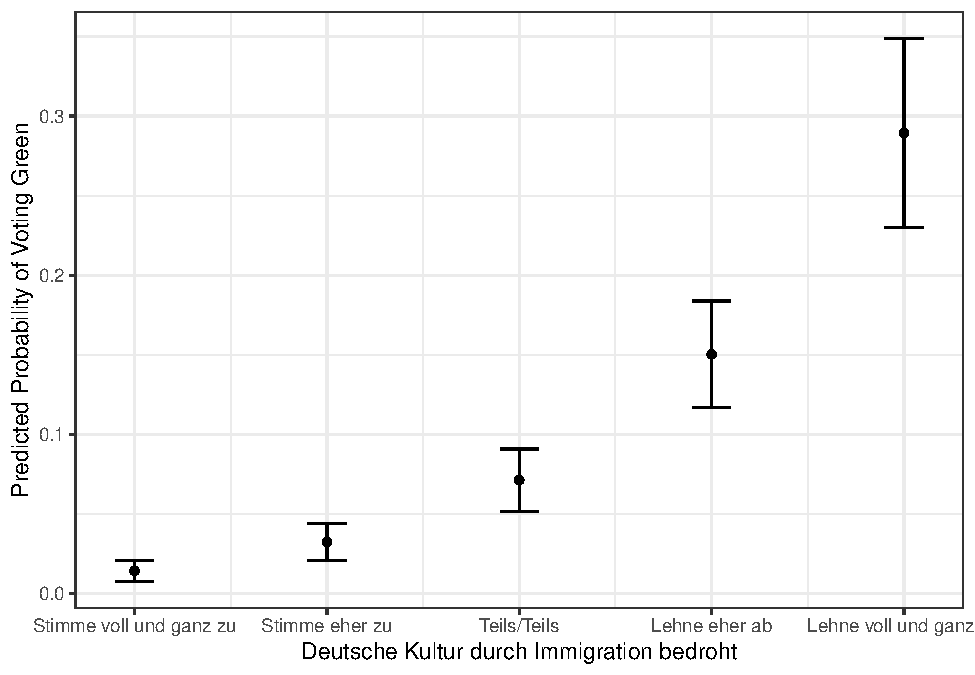
\includegraphics{AVCD_Final_Assignment-Edenhofer_files/figure-latex/gruene-immig-culture-threat-1.pdf}

\begin{Shaded}
\begin{Highlighting}[]
\NormalTok{gruene\_immig\_crime }\OtherTok{\textless{}{-}} \FunctionTok{glm}\NormalTok{(gruene\_21 }\SpecialCharTok{\textasciitilde{}}\NormalTok{ out\_group\_immig\_crime }\SpecialCharTok{+} \FunctionTok{I}\NormalTok{(out\_group\_immig\_crime}\SpecialCharTok{\^{}}\DecValTok{2}\NormalTok{) }\SpecialCharTok{+}\NormalTok{ household\_income }\SpecialCharTok{+}\NormalTok{ age }\SpecialCharTok{+}\NormalTok{ abitur\_factor }\SpecialCharTok{+}\NormalTok{ sex1 }\SpecialCharTok{+}\NormalTok{ urban\_rural\_factor }\SpecialCharTok{+}\NormalTok{ ostwest\_factor, }\AttributeTok{family =} \FunctionTok{binomial}\NormalTok{(}\AttributeTok{link =} \StringTok{"logit"}\NormalTok{), }\AttributeTok{data =}\NormalTok{ gles\_mod)}
\CommentTok{\# plot }
\FunctionTok{cplot}\NormalTok{(gruene\_immig\_crime, }\AttributeTok{x =} \StringTok{"out\_group\_immig\_crime"}\NormalTok{,}
      \AttributeTok{xvals =} \FunctionTok{seq}\NormalTok{(}\DecValTok{1}\NormalTok{, }\DecValTok{5}\NormalTok{, }\DecValTok{1}\NormalTok{), }\AttributeTok{draw =}\NormalTok{ F) }\SpecialCharTok{\%\textgreater{}\%}
  \FunctionTok{as\_tibble}\NormalTok{() }\SpecialCharTok{\%\textgreater{}\%}
  \FunctionTok{ggplot}\NormalTok{(}\FunctionTok{aes}\NormalTok{(}\AttributeTok{x =}\NormalTok{ xvals)) }\SpecialCharTok{+}
  \FunctionTok{geom\_point}\NormalTok{(}\FunctionTok{aes}\NormalTok{(}\AttributeTok{y =}\NormalTok{ yvals)) }\SpecialCharTok{+}
  \FunctionTok{geom\_errorbar}\NormalTok{(}\FunctionTok{aes}\NormalTok{(}\AttributeTok{ymin =}\NormalTok{ lower, }\AttributeTok{ymax =}\NormalTok{ upper), }\AttributeTok{width =} \FloatTok{0.2}\NormalTok{) }\SpecialCharTok{+}
  \FunctionTok{scale\_x\_continuous}\NormalTok{(}\StringTok{"Immigration erhoeht Kriminalitaet in BRD"}\NormalTok{, }
                     \AttributeTok{breaks =} \FunctionTok{seq}\NormalTok{(}\DecValTok{1}\NormalTok{, }\DecValTok{5}\NormalTok{, }\DecValTok{1}\NormalTok{), }
                     \AttributeTok{labels =} \FunctionTok{c}\NormalTok{(}\StringTok{"Stimme voll und ganz zu"}\NormalTok{, }\StringTok{"Stimme eher zu"}\NormalTok{, }
                                \StringTok{"Teils/Teils"}\NormalTok{, }\StringTok{"Lehne eher ab"}\NormalTok{, }
                                \StringTok{"Lehne voll und ganz ab"}\NormalTok{)) }\SpecialCharTok{+}
  \FunctionTok{labs}\NormalTok{(}\AttributeTok{y =} \StringTok{"Predicted Probability of Voting Green"}\NormalTok{) }\SpecialCharTok{+}
  \FunctionTok{ylim}\NormalTok{(}\FunctionTok{c}\NormalTok{(}\DecValTok{0}\NormalTok{, }\FloatTok{0.4}\NormalTok{)) }\SpecialCharTok{+}
  \FunctionTok{theme\_bw}\NormalTok{() }
\end{Highlighting}
\end{Shaded}

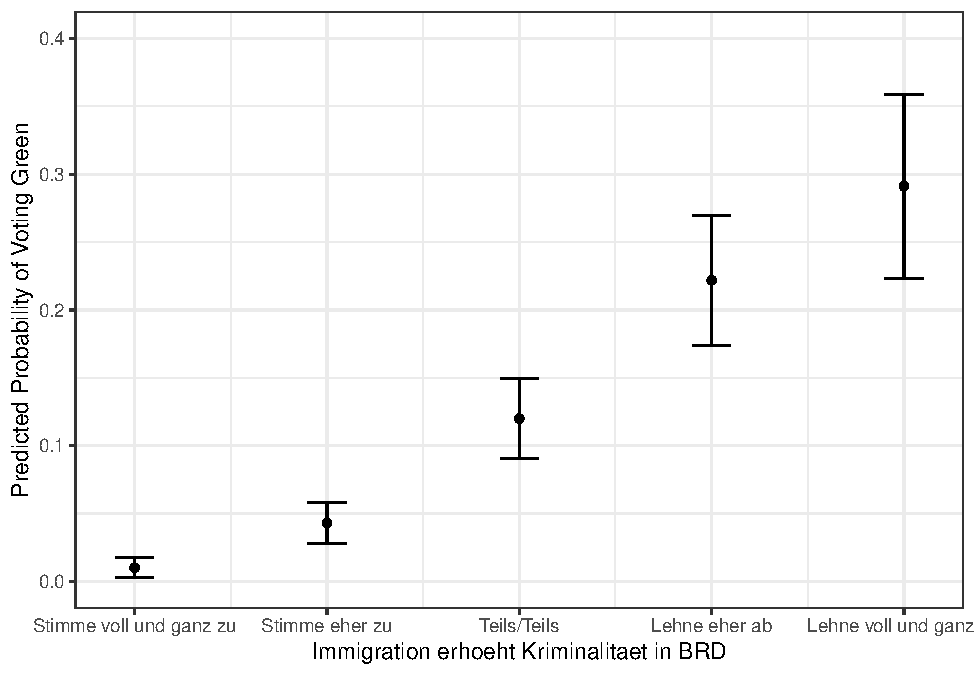
\includegraphics{AVCD_Final_Assignment-Edenhofer_files/figure-latex/gruene-immig-crime-1.pdf}

\begin{Shaded}
\begin{Highlighting}[]
\NormalTok{gruene\_majority }\OtherTok{\textless{}{-}} \FunctionTok{glm}\NormalTok{(gruene\_21 }\SpecialCharTok{\textasciitilde{}}\NormalTok{ out\_group\_majority\_will }\SpecialCharTok{+}\NormalTok{ household\_income }\SpecialCharTok{+}\NormalTok{ age }\SpecialCharTok{+}\NormalTok{ abitur\_factor }\SpecialCharTok{+}\NormalTok{ sex1 }\SpecialCharTok{+}\NormalTok{ urban\_rural\_factor }\SpecialCharTok{+}\NormalTok{ ostwest\_factor, }\AttributeTok{family =} \FunctionTok{binomial}\NormalTok{(}\AttributeTok{link =} \StringTok{"logit"}\NormalTok{), }\AttributeTok{data =}\NormalTok{ gles\_mod)}
\CommentTok{\# plot }
\FunctionTok{cplot}\NormalTok{(gruene\_majority, }\AttributeTok{x =} \StringTok{"out\_group\_majority\_will"}\NormalTok{, }
      \AttributeTok{xvals =} \FunctionTok{seq}\NormalTok{(}\DecValTok{1}\NormalTok{, }\DecValTok{5}\NormalTok{, }\DecValTok{1}\NormalTok{), }\AttributeTok{draw =}\NormalTok{ F) }\SpecialCharTok{\%\textgreater{}\%}
  \FunctionTok{as\_tibble}\NormalTok{() }\SpecialCharTok{\%\textgreater{}\%}
  \FunctionTok{ggplot}\NormalTok{(}\FunctionTok{aes}\NormalTok{(}\AttributeTok{x =}\NormalTok{ xvals)) }\SpecialCharTok{+}
  \FunctionTok{geom\_point}\NormalTok{(}\FunctionTok{aes}\NormalTok{(}\AttributeTok{y =}\NormalTok{ yvals)) }\SpecialCharTok{+}
  \FunctionTok{geom\_errorbar}\NormalTok{(}\FunctionTok{aes}\NormalTok{(}\AttributeTok{ymin =}\NormalTok{ lower, }\AttributeTok{ymax =}\NormalTok{ upper), }\AttributeTok{width =} \FloatTok{0.2}\NormalTok{) }\SpecialCharTok{+}
  \FunctionTok{scale\_x\_continuous}\NormalTok{(}\StringTok{"Wille der Mehrheit hat Vorrang"}\NormalTok{, }
                     \AttributeTok{breaks =} \FunctionTok{seq}\NormalTok{(}\DecValTok{1}\NormalTok{, }\DecValTok{5}\NormalTok{, }\DecValTok{1}\NormalTok{),}
                     \AttributeTok{labels =} \FunctionTok{c}\NormalTok{(}\StringTok{"Stimme voll und ganz zu"}\NormalTok{, }\StringTok{"Stimme eher zu"}\NormalTok{, }
                                \StringTok{"Teils/Teils"}\NormalTok{, }\StringTok{"Lehne eher ab"}\NormalTok{, }
                                \StringTok{"Lehne voll und ganz ab"}\NormalTok{)) }\SpecialCharTok{+}
  \FunctionTok{labs}\NormalTok{(}\AttributeTok{y =} \StringTok{"Predicted Probability of Voting Green"}\NormalTok{) }\SpecialCharTok{+}
  \FunctionTok{theme\_bw}\NormalTok{()}
\end{Highlighting}
\end{Shaded}

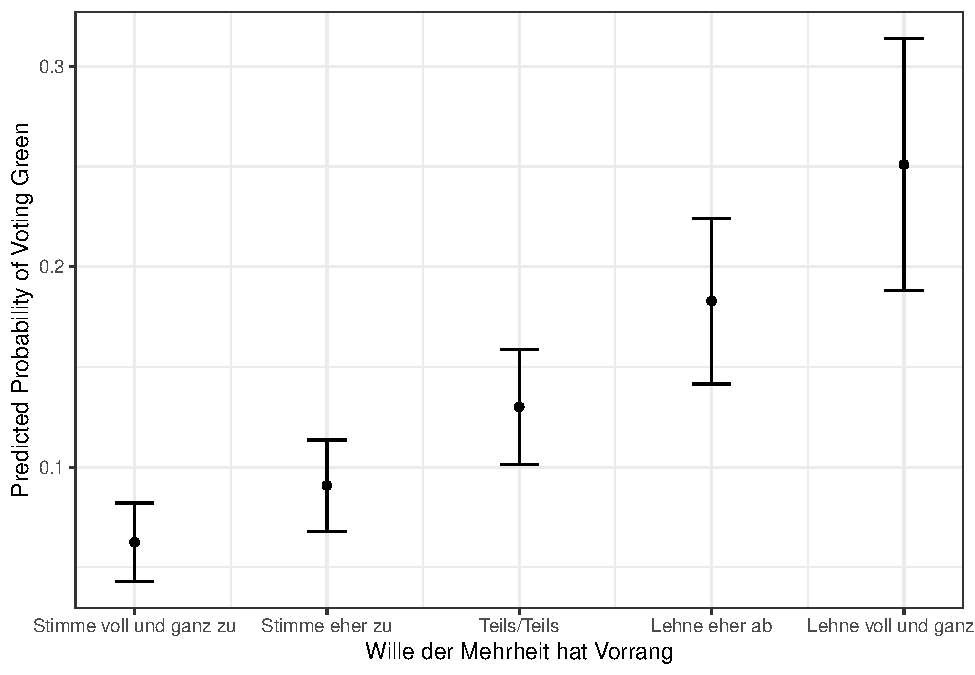
\includegraphics{AVCD_Final_Assignment-Edenhofer_files/figure-latex/gruene-majority-will-1.pdf}

\hypertarget{further-analysis}{%
\section{Further analysis}\label{further-analysis}}

Valence -\textgreater{} motivation: Baerbock's campaign

How can we measure valence vs spatial distance?

Who punished the Greens because of Baerbock? Who punished the CDU/CSU
because of Laschet? (Lachet and so on) -\textgreater{} Those who are
struggling / hard times.

-\textgreater{} egoistic vs sociotropic motivations/evaluations?
-\textgreater{} egoistic evaluations matter more when one is
ideologically closer to a candidate/party; spell this out
-\textgreater{} sociotropic evaluations matter more when one thinks
highly of a candidate

\begin{Shaded}
\begin{Highlighting}[]
\NormalTok{ego\_socio\_model1 }\OtherTok{\textless{}{-}} \FunctionTok{glm}\NormalTok{(union\_21 }\SpecialCharTok{\textasciitilde{}}\NormalTok{ econ\_current\_personal}\SpecialCharTok{*}\NormalTok{econ\_current\_eval\_general}\SpecialCharTok{*}\NormalTok{scale\_pol\_lasceht,}
                       \AttributeTok{family =} \FunctionTok{binomial}\NormalTok{(}\AttributeTok{link =} \StringTok{"logit"}\NormalTok{),}
                       \AttributeTok{data =}\NormalTok{ gles\_mod)}
\NormalTok{ego\_socio\_model2 }\OtherTok{\textless{}{-}} \FunctionTok{glm}\NormalTok{(union\_21 }\SpecialCharTok{\textasciitilde{}}\NormalTok{ econ\_current\_personal}\SpecialCharTok{*}\NormalTok{econ\_current\_eval\_general}\SpecialCharTok{*}\NormalTok{scale\_pol\_lasceht }\SpecialCharTok{+}\NormalTok{ distance\_cdu }\SpecialCharTok{+}\NormalTok{  household\_income }\SpecialCharTok{+}\NormalTok{ age,}
                       \AttributeTok{family =} \FunctionTok{binomial}\NormalTok{(}\AttributeTok{link =} \StringTok{"logit"}\NormalTok{),}
                       \AttributeTok{data =}\NormalTok{ gles\_mod)}
\NormalTok{ego\_socio\_model3 }\OtherTok{\textless{}{-}} \FunctionTok{glm}\NormalTok{(union\_21 }\SpecialCharTok{\textasciitilde{}}\NormalTok{ distance\_cdu}\SpecialCharTok{*}\NormalTok{econ\_current\_personal }\SpecialCharTok{+}\NormalTok{ econ\_current\_eval\_general}\SpecialCharTok{*}\NormalTok{scale\_pol\_lasceht }\SpecialCharTok{+}\NormalTok{  household\_income }\SpecialCharTok{+}\NormalTok{ age }\SpecialCharTok{+}\NormalTok{ abitur\_factor }\SpecialCharTok{+}\NormalTok{ sex1,}
                       \AttributeTok{family =} \FunctionTok{binomial}\NormalTok{(}\AttributeTok{link =} \StringTok{"logit"}\NormalTok{),}
                       \AttributeTok{data =}\NormalTok{ gles\_mod)}
\NormalTok{ego\_socio\_model4 }\OtherTok{\textless{}{-}} \FunctionTok{glm}\NormalTok{(union\_21 }\SpecialCharTok{\textasciitilde{}}\NormalTok{ distance\_cdu}\SpecialCharTok{*}\NormalTok{econ\_current\_personal }\SpecialCharTok{+}\NormalTok{ econ\_current\_eval\_general}\SpecialCharTok{*}\NormalTok{scale\_pol\_lasceht }\SpecialCharTok{+}\NormalTok{  household\_income }\SpecialCharTok{+}\NormalTok{ age }\SpecialCharTok{+}\NormalTok{ abitur\_factor }\SpecialCharTok{+}\NormalTok{ sex1 }\SpecialCharTok{+}\NormalTok{ urban\_rural\_factor }\SpecialCharTok{+}\NormalTok{ ostwest\_factor,}
                       \AttributeTok{family =} \FunctionTok{binomial}\NormalTok{(}\AttributeTok{link =} \StringTok{"logit"}\NormalTok{),}
                       \AttributeTok{data =}\NormalTok{ gles\_mod)}
\NormalTok{ego\_socio\_model5 }\OtherTok{\textless{}{-}} \FunctionTok{glm}\NormalTok{(union\_21 }\SpecialCharTok{\textasciitilde{}}\NormalTok{ distance\_cdu}\SpecialCharTok{*}\NormalTok{econ\_current\_personal}\SpecialCharTok{*}\NormalTok{scale\_pol\_lasceht }\SpecialCharTok{+}\NormalTok{ econ\_current\_eval\_general}\SpecialCharTok{*}\NormalTok{scale\_pol\_lasceht }\SpecialCharTok{+}\NormalTok{  household\_income }\SpecialCharTok{+}\NormalTok{ age }\SpecialCharTok{+}\NormalTok{ abitur\_factor }\SpecialCharTok{+}\NormalTok{ sex1 }\SpecialCharTok{+}\NormalTok{ urban\_rural\_factor }\SpecialCharTok{+}\NormalTok{ ostwest\_factor,}
                       \AttributeTok{family =} \FunctionTok{binomial}\NormalTok{(}\AttributeTok{link =} \StringTok{"logit"}\NormalTok{),}
                       \AttributeTok{data =}\NormalTok{ gles\_mod)}
\NormalTok{ego\_socio\_model6 }\OtherTok{\textless{}{-}} \FunctionTok{glm}\NormalTok{(union\_21 }\SpecialCharTok{\textasciitilde{}}\NormalTok{ distance\_cdu }\SpecialCharTok{+}\NormalTok{ econ\_current\_eval\_general}\SpecialCharTok{*}\NormalTok{econ\_current\_personal}\SpecialCharTok{*}\NormalTok{scale\_pol\_lasceht }\SpecialCharTok{+}\NormalTok{ household\_income }\SpecialCharTok{+}\NormalTok{ age }\SpecialCharTok{+}\NormalTok{ abitur\_factor }\SpecialCharTok{+}\NormalTok{ sex1 }\SpecialCharTok{+}\NormalTok{ urban\_rural\_factor }\SpecialCharTok{+}\NormalTok{ ostwest\_factor,}
                       \AttributeTok{family =} \FunctionTok{binomial}\NormalTok{(}\AttributeTok{link =} \StringTok{"logit"}\NormalTok{),}
                       \AttributeTok{data =}\NormalTok{ gles\_mod)}
\CommentTok{\# modelsummary}
\FunctionTok{modelsummary}\NormalTok{(}\FunctionTok{list}\NormalTok{(ego\_socio\_model1, ego\_socio\_model2, ego\_socio\_model3, }
\NormalTok{                  ego\_socio\_model4, ego\_socio\_model5),}
             \AttributeTok{estimate =} \StringTok{"\{estimate\}\{stars\}"}\NormalTok{)}
\end{Highlighting}
\end{Shaded}

\begin{table}
\centering
\begin{tabular}[t]{lccccc}
\toprule
  & (1) & (2) & (3) & (4) & (5)\\
\midrule
(Intercept) & \num{-2.121}* & \num{-4.105}** & \num{-3.769}*** & \num{-4.012}*** & \num{-3.372}***\\
 & (\num{1.067}) & (\num{1.396}) & (\num{0.697}) & (\num{0.713}) & (\num{0.750})\\
econ\_current\_personal & \num{-0.110} & \num{0.097} & \num{-0.084} & \num{-0.088} & \num{-0.380}+\\
 & (\num{0.457}) & (\num{0.582}) & (\num{0.106}) & (\num{0.106}) & (\num{0.199})\\
econ\_current\_eval\_general & \num{-0.304} & \num{0.166} & \num{-0.014} & \num{-0.027} & \num{-0.005}\\
 & (\num{0.406}) & (\num{0.495}) & (\num{0.177}) & (\num{0.179}) & (\num{0.191})\\
scale\_pol\_lasceht & \num{0.363}+ & \num{0.490}* & \num{0.410}*** & \num{0.403}*** & \num{0.265}**\\
 & (\num{0.189}) & (\num{0.228}) & (\num{0.081}) & (\num{0.082}) & (\num{0.094})\\
econ\_current\_personal × econ\_current\_eval\_general & \num{0.034} & \num{-0.055} &  &  & \\
 & (\num{0.159}) & (\num{0.201}) &  &  & \\
econ\_current\_personal × scale\_pol\_lasceht & \num{0.013} & \num{-0.027} &  &  & \num{0.068}+\\
 & (\num{0.082}) & (\num{0.100}) &  &  & (\num{0.034})\\
econ\_current\_eval\_general × scale\_pol\_lasceht & \num{-0.004} & \num{-0.102} & \num{-0.054}+ & \num{-0.050} & \\
 & (\num{0.074}) & (\num{0.089}) & (\num{0.032}) & (\num{0.032}) & \\
econ\_current\_personal × econ\_current\_eval\_general × scale\_pol\_lasceht & \num{-0.006} & \num{0.017} &  &  & \\
 & (\num{0.029}) & (\num{0.036}) &  &  & \\
distance\_cdu &  & \num{-0.138}*** & \num{-0.213}*** & \num{-0.210}*** & \num{-0.345}***\\
 &  & (\num{0.015}) & (\num{0.038}) & (\num{0.038}) & (\num{0.061})\\
household\_income &  & \num{0.062}* & \num{0.076}* & \num{0.072}* & \num{0.070}*\\
 &  & (\num{0.031}) & (\num{0.032}) & (\num{0.032}) & (\num{0.032})\\
age &  & \num{0.022}*** & \num{0.019}*** & \num{0.019}*** & \num{0.019}***\\
 &  & (\num{0.004}) & (\num{0.004}) & (\num{0.004}) & (\num{0.004})\\
abitur\_factorno\_abitur &  &  & \num{0.386}** & \num{0.351}* & \num{0.335}*\\
 &  &  & (\num{0.139}) & (\num{0.141}) & (\num{0.141})\\
sex1female &  &  & \num{-0.090} & \num{-0.077} & \num{-0.076}\\
 &  &  & (\num{0.123}) & (\num{0.124}) & (\num{0.124})\\
distance\_cdu × econ\_current\_personal &  &  & \num{0.035}* & \num{0.034}* & \num{0.085}***\\
 &  &  & (\num{0.014}) & (\num{0.014}) & (\num{0.017})\\
urban\_rural\_factor2 &  &  &  & \num{0.262} & \num{0.279}\\
 &  &  &  & (\num{0.210}) & (\num{0.210})\\
urban\_rural\_factor3 &  &  &  & \num{0.313}+ & \num{0.335}+\\
 &  &  &  & (\num{0.182}) & (\num{0.183})\\
urban\_rural\_factor4 &  &  &  & \num{0.331}+ & \num{0.344}+\\
 &  &  &  & (\num{0.188}) & (\num{0.188})\\
urban\_rural\_factor5 &  &  &  & \num{0.634} & \num{0.586}\\
 &  &  &  & (\num{0.484}) & (\num{0.492})\\
ostwest\_factorwest &  &  &  & \num{0.082} & \num{0.078}\\
 &  &  &  & (\num{0.139}) & (\num{0.140})\\
distance\_cdu × scale\_pol\_lasceht &  &  &  &  & \num{0.035}***\\
 &  &  &  &  & (\num{0.010})\\
scale\_pol\_lasceht × econ\_current\_eval\_general &  &  &  &  & \num{-0.056}\\
 &  &  &  &  & (\num{0.035})\\
distance\_cdu × econ\_current\_personal × scale\_pol\_lasceht &  &  &  &  & \num{-0.015}***\\
 &  &  &  &  & (\num{0.004})\\
\midrule
Num.Obs. & \num{2792} & \num{2225} & \num{2221} & \num{2211} & \num{2211}\\
AIC & \num{2473.1} & \num{1732.5} & \num{1718.2} & \num{1715.3} & \num{1709.5}\\
BIC & \num{2520.5} & \num{1795.3} & \num{1780.9} & \num{1806.6} & \num{1817.8}\\
Log.Lik. & \num{-1228.528} & \num{-855.242} & \num{-848.079} & \num{-841.671} & \num{-835.737}\\
RMSE & \num{0.37} & \num{0.35} & \num{0.35} & \num{0.35} & \num{0.35}\\
\bottomrule
\end{tabular}
\end{table}

\begin{Shaded}
\begin{Highlighting}[]
\NormalTok{ego\_socio\_model11 }\OtherTok{\textless{}{-}} \FunctionTok{glm}\NormalTok{(union\_21 }\SpecialCharTok{\textasciitilde{}}\NormalTok{ distance\_cdu}\SpecialCharTok{*}\NormalTok{scale\_pol\_lasceht }\SpecialCharTok{+}\NormalTok{ sex }\SpecialCharTok{+}\NormalTok{ household\_income }\SpecialCharTok{+}\NormalTok{ urban\_rural }\SpecialCharTok{+}\NormalTok{ ostwest\_factor }\SpecialCharTok{+}\NormalTok{ age,}
                       \AttributeTok{family =} \FunctionTok{binomial}\NormalTok{(}\AttributeTok{link =} \StringTok{"logit"}\NormalTok{),}
                       \AttributeTok{data =}\NormalTok{ gles\_mod)}
\NormalTok{ego\_socio\_model12 }\OtherTok{\textless{}{-}} \FunctionTok{glm}\NormalTok{(spd\_21 }\SpecialCharTok{\textasciitilde{}}\NormalTok{ distance\_spd}\SpecialCharTok{*}\NormalTok{scale\_pol\_scholz }\SpecialCharTok{+}\NormalTok{ sex }\SpecialCharTok{+}\NormalTok{ household\_income }\SpecialCharTok{+}\NormalTok{ urban\_rural }\SpecialCharTok{+}\NormalTok{ ostwest\_factor }\SpecialCharTok{+}\NormalTok{ age,}
                       \AttributeTok{family =} \FunctionTok{binomial}\NormalTok{(}\AttributeTok{link =} \StringTok{"logit"}\NormalTok{),}
                       \AttributeTok{data =}\NormalTok{ gles\_mod)}
\NormalTok{ego\_socio\_model13 }\OtherTok{\textless{}{-}} \FunctionTok{glm}\NormalTok{(gruene\_21 }\SpecialCharTok{\textasciitilde{}}\NormalTok{ distance\_green}\SpecialCharTok{*}\NormalTok{scale\_pol\_baerbock }\SpecialCharTok{+}\NormalTok{ sex }\SpecialCharTok{+}\NormalTok{ household\_income }\SpecialCharTok{+}\NormalTok{ urban\_rural }\SpecialCharTok{+}\NormalTok{ ostwest\_factor }\SpecialCharTok{+}\NormalTok{ age,}
                       \AttributeTok{family =} \FunctionTok{binomial}\NormalTok{(}\AttributeTok{link =} \StringTok{"logit"}\NormalTok{),}
                       \AttributeTok{data =}\NormalTok{ gles\_mod)}
\NormalTok{ego\_socio\_model14 }\OtherTok{\textless{}{-}} \FunctionTok{glm}\NormalTok{(afd\_21 }\SpecialCharTok{\textasciitilde{}}\NormalTok{ distance\_afd }\SpecialCharTok{+}\NormalTok{ sex }\SpecialCharTok{+}\NormalTok{ household\_income }\SpecialCharTok{+}\NormalTok{ urban\_rural }\SpecialCharTok{+}\NormalTok{ ostwest\_factor }\SpecialCharTok{+}\NormalTok{ age,}
                       \AttributeTok{family =} \FunctionTok{binomial}\NormalTok{(}\AttributeTok{link =} \StringTok{"logit"}\NormalTok{),}
                       \AttributeTok{data =}\NormalTok{ gles\_mod)}
\NormalTok{ego\_socio\_model15 }\OtherTok{\textless{}{-}} \FunctionTok{glm}\NormalTok{(fdp\_21 }\SpecialCharTok{\textasciitilde{}}\NormalTok{ econ\_current\_personal}\SpecialCharTok{*}\NormalTok{econ\_current\_eval\_general,}
                       \AttributeTok{family =} \FunctionTok{binomial}\NormalTok{(}\AttributeTok{link =} \StringTok{"logit"}\NormalTok{),}
                       \AttributeTok{data =}\NormalTok{ gles\_mod)}

\CommentTok{\# modelsummar\textless{}}
\FunctionTok{modelsummary}\NormalTok{(}\FunctionTok{list}\NormalTok{(ego\_socio\_model11, ego\_socio\_model12, ego\_socio\_model13, ego\_socio\_model14), }
             \AttributeTok{estimate =} \StringTok{"\{estimate\}\{stars\}"}\NormalTok{,}
             \AttributeTok{output =} \StringTok{"kableExtra"}\NormalTok{) }\SpecialCharTok{\%\textgreater{}\%}
\NormalTok{  kableExtra}\SpecialCharTok{::}\FunctionTok{kable\_styling}\NormalTok{(}\AttributeTok{latex\_options =} \StringTok{"scale\_down"}\NormalTok{)}
\end{Highlighting}
\end{Shaded}

\begin{table}
\centering
\resizebox{\linewidth}{!}{
\begin{tabular}[t]{lcccc}
\toprule
  & (1) & (2) & (3) & (4)\\
\midrule
(Intercept) & \num{-4.012}*** & \num{-6.204}*** & \num{-4.509}*** & \num{1.651}*\\
 & (\num{0.491}) & (\num{0.524}) & (\num{0.538}) & (\num{0.737})\\
distance\_cdu & \num{-0.138}*** &  &  & \\
 & (\num{0.030}) &  &  & \\
scale\_pol\_lasceht & \num{0.287}*** &  &  & \\
 & (\num{0.027}) &  &  & \\
sex & \num{-0.119} & \num{-0.126} & \num{0.215}+ & \num{-0.269}\\
 & (\num{0.121}) & (\num{0.113}) & (\num{0.128}) & (\num{0.229})\\
household\_income & \num{0.060}* & \num{-0.041} & \num{0.065}* & \num{-0.179}***\\
 & (\num{0.028}) & (\num{0.025}) & (\num{0.028}) & (\num{0.045})\\
urban\_rural & \num{0.111}* & \num{0.015} & \num{-0.047} & \num{0.172}+\\
 & (\num{0.055}) & (\num{0.049}) & (\num{0.056}) & (\num{0.100})\\
ostwest\_factorwest & \num{0.092} & \num{0.112} & \num{0.503}** & \num{-1.011}***\\
 & (\num{0.137}) & (\num{0.124}) & (\num{0.153}) & (\num{0.216})\\
age & \num{0.022}*** & \num{0.009}** & \num{-0.030}*** & \num{0.001}\\
 & (\num{0.004}) & (\num{0.003}) & (\num{0.004}) & (\num{0.007})\\
distance\_cdu × scale\_pol\_lasceht & \num{0.000} &  &  & \\
 & (\num{0.006}) &  &  & \\
distance\_spd &  & \num{0.012} &  & \\
 &  & (\num{0.031}) &  & \\
scale\_pol\_scholz &  & \num{0.678}*** &  & \\
 &  & (\num{0.043}) &  & \\
distance\_spd × scale\_pol\_scholz &  & \num{-0.007}* &  & \\
 &  & (\num{0.004}) &  & \\
distance\_green &  &  & \num{-0.106} & \\
 &  &  & (\num{0.074}) & \\
scale\_pol\_baerbock &  &  & \num{0.564}*** & \\
 &  &  & (\num{0.043}) & \\
distance\_green × scale\_pol\_baerbock &  &  & \num{-0.005} & \\
 &  &  & (\num{0.010}) & \\
distance\_afd &  &  &  & \num{-0.183}***\\
 &  &  &  & (\num{0.016})\\
\midrule
Num.Obs. & \num{2239} & \num{2233} & \num{2224} & \num{2225}\\
AIC & \num{1754.9} & \num{1974.2} & \num{1539.0} & \num{596.6}\\
BIC & \num{1806.3} & \num{2025.6} & \num{1590.4} & \num{636.5}\\
Log.Lik. & \num{-868.431} & \num{-978.124} & \num{-760.511} & \num{-291.289}\\
RMSE & \num{0.35} & \num{0.38} & \num{0.33} & \num{0.20}\\
\bottomrule
\end{tabular}}
\end{table}

\begin{Shaded}
\begin{Highlighting}[]
\NormalTok{afd\_gender1 }\OtherTok{\textless{}{-}} \FunctionTok{glm}\NormalTok{(afd\_21 }\SpecialCharTok{\textasciitilde{}}\NormalTok{ gender\_too\_far\_factor }\SpecialCharTok{+}\NormalTok{ age }\SpecialCharTok{+}\NormalTok{ abitur\_factor }\SpecialCharTok{+}\NormalTok{ sex1 }\SpecialCharTok{+}\NormalTok{ urban\_rural\_factor }\SpecialCharTok{+}\NormalTok{ ostwest\_factor, }
                  \AttributeTok{family =} \FunctionTok{binomial}\NormalTok{(}\AttributeTok{link =} \StringTok{"logit"}\NormalTok{), }
                  \AttributeTok{data =}\NormalTok{ gles\_mod)}
\NormalTok{afd\_gender2 }\OtherTok{\textless{}{-}} \FunctionTok{glm}\NormalTok{(afd\_21 }\SpecialCharTok{\textasciitilde{}}\NormalTok{ gender\_too\_far\_factor}\SpecialCharTok{*}\NormalTok{sex1 }\SpecialCharTok{+}\NormalTok{ age }\SpecialCharTok{+}\NormalTok{ abitur\_factor }\SpecialCharTok{+}\NormalTok{  urban\_rural\_factor }\SpecialCharTok{+}\NormalTok{ ostwest\_factor, }
                  \AttributeTok{family =} \FunctionTok{binomial}\NormalTok{(}\AttributeTok{link =} \StringTok{"logit"}\NormalTok{), }
                  \AttributeTok{data =}\NormalTok{ gles\_mod)}
\NormalTok{afd\_gender3 }\OtherTok{\textless{}{-}} \FunctionTok{glm}\NormalTok{(afd\_21 }\SpecialCharTok{\textasciitilde{}}\NormalTok{ gender\_too\_far\_factor}\SpecialCharTok{*}\NormalTok{sex1 }\SpecialCharTok{+}\NormalTok{ age }\SpecialCharTok{+}\NormalTok{ abitur\_factor }\SpecialCharTok{+}\NormalTok{  urban\_rural\_factor }\SpecialCharTok{+}\NormalTok{ ostwest\_factor }\SpecialCharTok{+}\NormalTok{ unemployed\_dummy\_factor, }
                  \AttributeTok{family =} \FunctionTok{binomial}\NormalTok{(}\AttributeTok{link =} \StringTok{"logit"}\NormalTok{), }
                  \AttributeTok{data =}\NormalTok{ gles\_mod)}
\NormalTok{afd\_gender4 }\OtherTok{\textless{}{-}} \FunctionTok{glm}\NormalTok{(afd\_21 }\SpecialCharTok{\textasciitilde{}}\NormalTok{ gender\_too\_far\_factor}\SpecialCharTok{*}\NormalTok{sex1}\SpecialCharTok{*}\NormalTok{unemployed\_dummy }\SpecialCharTok{+}\NormalTok{ age }\SpecialCharTok{+}\NormalTok{ abitur\_factor }\SpecialCharTok{+}\NormalTok{  urban\_rural\_factor }\SpecialCharTok{+}\NormalTok{ ostwest\_factor, }
                  \AttributeTok{family =} \FunctionTok{binomial}\NormalTok{(}\AttributeTok{link =} \StringTok{"logit"}\NormalTok{), }
                  \AttributeTok{data =}\NormalTok{ gles\_mod)}
\NormalTok{afd\_gender5 }\OtherTok{\textless{}{-}} \FunctionTok{glm}\NormalTok{(afd\_21 }\SpecialCharTok{\textasciitilde{}}\NormalTok{ gender\_too\_far\_factor}\SpecialCharTok{*}\NormalTok{sex1}\SpecialCharTok{*}\NormalTok{econ\_current\_personal }\SpecialCharTok{+}\NormalTok{ age }\SpecialCharTok{+}\NormalTok{ abitur\_factor }\SpecialCharTok{+}\NormalTok{  urban\_rural\_factor }\SpecialCharTok{+}\NormalTok{ ostwest\_factor, }
                  \AttributeTok{family =} \FunctionTok{binomial}\NormalTok{(}\AttributeTok{link =} \StringTok{"logit"}\NormalTok{), }
                  \AttributeTok{data =}\NormalTok{ gles\_mod)}

\CommentTok{\# modelsummary }
\FunctionTok{modelsummary}\NormalTok{(}\FunctionTok{list}\NormalTok{(afd\_gender1, afd\_gender2, afd\_gender3, afd\_gender5), }
             \AttributeTok{estimate =} \StringTok{"\{estimate\}\{stars\}"}\NormalTok{, }
             \AttributeTok{output =} \StringTok{"kableExtra"}\NormalTok{) }\SpecialCharTok{\%\textgreater{}\%}
\NormalTok{  kableExtra}\SpecialCharTok{::}\FunctionTok{kable\_styling}\NormalTok{(}\AttributeTok{latex\_options =} \StringTok{"scale\_down"}\NormalTok{)}
\end{Highlighting}
\end{Shaded}

\begin{table}
\centering
\resizebox{\linewidth}{!}{
\begin{tabular}[t]{lcccc}
\toprule
  & (1) & (2) & (3) & (4)\\
\midrule
(Intercept) & \num{-0.510} & \num{-0.511} & \num{-0.584} & \num{-0.175}\\
 & (\num{0.439}) & (\num{0.469}) & (\num{0.481}) & (\num{0.968})\\
gender\_too\_far\_factor2 & \num{-0.997}** & \num{-0.929}* & \num{-0.968}* & \num{-1.446}\\
 & (\num{0.343}) & (\num{0.410}) & (\num{0.411}) & (\num{1.135})\\
gender\_too\_far\_factor3 & \num{-1.498}*** & \num{-1.548}*** & \num{-1.601}*** & \num{-2.611}*\\
 & (\num{0.318}) & (\num{0.377}) & (\num{0.378}) & (\num{1.071})\\
gender\_too\_far\_factor4 & \num{-2.380}*** & \num{-2.243}*** & \num{-2.312}*** & \num{-4.777}***\\
 & (\num{0.329}) & (\num{0.390}) & (\num{0.392}) & (\num{1.163})\\
gender\_too\_far\_factor5 & \num{-2.887}*** & \num{-3.493}*** & \num{-3.766}*** & \num{-5.305}**\\
 & (\num{0.372}) & (\num{0.565}) & (\num{0.608}) & (\num{1.668})\\
age & \num{-0.004} & \num{-0.004} & \num{-0.003} & \num{-0.001}\\
 & (\num{0.005}) & (\num{0.005}) & (\num{0.005}) & (\num{0.005})\\
abitur\_factorno\_abitur & \num{0.922}*** & \num{0.925}*** & \num{0.889}*** & \num{0.713}**\\
 & (\num{0.213}) & (\num{0.213}) & (\num{0.217}) & (\num{0.218})\\
sex1female & \num{-0.373}* & \num{-0.418} & \num{-0.507} & \num{-1.647}\\
 & (\num{0.171}) & (\num{0.641}) & (\num{0.638}) & (\num{1.969})\\
urban\_rural\_factor2 & \num{0.243} & \num{0.258} & \num{0.303} & \num{0.261}\\
 & (\num{0.294}) & (\num{0.295}) & (\num{0.301}) & (\num{0.302})\\
urban\_rural\_factor3 & \num{0.200} & \num{0.212} & \num{0.205} & \num{0.218}\\
 & (\num{0.250}) & (\num{0.251}) & (\num{0.259}) & (\num{0.257})\\
urban\_rural\_factor4 & \num{0.420} & \num{0.433}+ & \num{0.484}+ & \num{0.404}\\
 & (\num{0.257}) & (\num{0.257}) & (\num{0.264}) & (\num{0.263})\\
urban\_rural\_factor5 & \num{1.301}* & \num{1.366}* & \num{0.855} & \num{1.368}*\\
 & (\num{0.552}) & (\num{0.558}) & (\num{0.652}) & (\num{0.565})\\
ostwest\_factorwest & \num{-1.311}*** & \num{-1.319}*** & \num{-1.255}*** & \num{-1.305}***\\
 & (\num{0.167}) & (\num{0.167}) & (\num{0.172}) & (\num{0.172})\\
gender\_too\_far\_factor2 × sex1female &  & \num{-0.179} & \num{-0.124} & \num{-2.211}\\
 &  & (\num{0.757}) & (\num{0.760}) & (\num{2.441})\\
gender\_too\_far\_factor3 × sex1female &  & \num{0.161} & \num{0.239} & \num{-0.834}\\
 &  & (\num{0.702}) & (\num{0.705}) & (\num{2.229})\\
gender\_too\_far\_factor4 × sex1female &  & \num{-0.373} & \num{-0.314} & \num{0.669}\\
 &  & (\num{0.728}) & (\num{0.730}) & (\num{2.330})\\
gender\_too\_far\_factor5 × sex1female &  & \num{0.974} & \num{1.172} & \num{0.057}\\
 &  & (\num{0.831}) & (\num{0.866}) & (\num{2.619})\\
unemployed\_dummy\_factor1 &  &  & \num{0.665}** & \\
 &  &  & (\num{0.257}) & \\
econ\_current\_personal &  &  &  & \num{-0.148}\\
 &  &  &  & (\num{0.361})\\
gender\_too\_far\_factor2 × econ\_current\_personal &  &  &  & \num{0.233}\\
 &  &  &  & (\num{0.451})\\
gender\_too\_far\_factor3 × econ\_current\_personal &  &  &  & \num{0.454}\\
 &  &  &  & (\num{0.422})\\
gender\_too\_far\_factor4 × econ\_current\_personal &  &  &  & \num{1.040}*\\
 &  &  &  & (\num{0.446})\\
gender\_too\_far\_factor5 × econ\_current\_personal &  &  &  & \num{0.764}\\
 &  &  &  & (\num{0.626})\\
sex1female × econ\_current\_personal &  &  &  & \num{0.465}\\
 &  &  &  & (\num{0.677})\\
gender\_too\_far\_factor2 × sex1female × econ\_current\_personal &  &  &  & \num{0.724}\\
 &  &  &  & (\num{0.836})\\
gender\_too\_far\_factor3 × sex1female × econ\_current\_personal &  &  &  & \num{0.384}\\
 &  &  &  & (\num{0.772})\\
gender\_too\_far\_factor4 × sex1female × econ\_current\_personal &  &  &  & \num{-0.458}\\
 &  &  &  & (\num{0.797})\\
gender\_too\_far\_factor5 × sex1female × econ\_current\_personal &  &  &  & \num{0.176}\\
 &  &  &  & (\num{0.896})\\
\midrule
Num.Obs. & \num{2703} & \num{2703} & \num{2581} & \num{2701}\\
AIC & \num{1145.5} & \num{1148.1} & \num{1081.3} & \num{1099.9}\\
BIC & \num{1222.3} & \num{1248.4} & \num{1186.7} & \num{1259.3}\\
Log.Lik. & \num{-559.768} & \num{-557.047} & \num{-522.647} & \num{-522.957}\\
RMSE & \num{0.24} & \num{0.24} & \num{0.23} & \num{0.23}\\
\bottomrule
\end{tabular}}
\end{table}

\end{document}
